\pdfminorversion=7
%DIF LATEXDIFF DIFFERENCE FILE
%DIF DEL ../baseline/Causal_WeatherGraph_elsarticle.tex   Sat Jul 18 06:32:43 2026
%DIF ADD Causal_WeatherGraph_revised.tex                  Sat Oct  3 09:53:51 2026
\documentclass[preprint,12pt]{elsarticle}

\usepackage[T1]{fontenc}
\usepackage[utf8]{inputenc}
\usepackage{lmodern}
\usepackage{amssymb}
\usepackage{amsmath}
\usepackage{booktabs}
\usepackage{array}
%DIF 11a11
\usepackage{graphicx}
 %DIF > 
%DIF -------
\usepackage[colorlinks=true,linkcolor=blue,citecolor=blue,urlcolor=blue]{hyperref}
\hypersetup{pdfauthor={Xinchen Geng}}

%DIF 13c14
%DIF < \biboptions{numbers,sort&compress}
%DIF -------
\biboptions{numbers}
 %DIF > 
%DIF -------

\setlength{\emergencystretch}{2em}
\makeatletter
\setlength{\@fptop}{0pt}
\setlength{\@fpsep}{14pt}
\setlength{\@fpbot}{0pt plus 1fil}
\makeatother
\renewcommand{\topfraction}{0.95}
\renewcommand{\bottomfraction}{0.95}
\renewcommand{\textfraction}{0.06}
\renewcommand{\floatpagefraction}{0.80}

\journal{Information Sciences}

 %DIF > 
%DIF PREAMBLE EXTENSION ADDED BY LATEXDIFF
%DIF UNDERLINE PREAMBLE %DIF PREAMBLE
\RequirePackage[normalem]{ulem} %DIF PREAMBLE
\RequirePackage{color}\definecolor{RED}{rgb}{1,0,0}\definecolor{BLUE}{rgb}{0,0,1} %DIF PREAMBLE
\providecommand{\DIFaddtex}[1]{{\protect\color{blue}\uwave{#1}}} %DIF PREAMBLE
\providecommand{\DIFdeltex}[1]{{\protect\color{red}\sout{#1}}} %DIF PREAMBLE
%DIF SAFE PREAMBLE %DIF PREAMBLE
\providecommand{\DIFaddbegin}{} %DIF PREAMBLE
\providecommand{\DIFaddend}{} %DIF PREAMBLE
\providecommand{\DIFdelbegin}{} %DIF PREAMBLE
\providecommand{\DIFdelend}{} %DIF PREAMBLE
\providecommand{\DIFmodbegin}{} %DIF PREAMBLE
\providecommand{\DIFmodend}{} %DIF PREAMBLE
%DIF FLOATSAFE PREAMBLE %DIF PREAMBLE
\providecommand{\DIFaddFL}[1]{\DIFadd{#1}} %DIF PREAMBLE
\providecommand{\DIFdelFL}[1]{\DIFdel{#1}} %DIF PREAMBLE
\providecommand{\DIFaddbeginFL}{} %DIF PREAMBLE
\providecommand{\DIFaddendFL}{} %DIF PREAMBLE
\providecommand{\DIFdelbeginFL}{} %DIF PREAMBLE
\providecommand{\DIFdelendFL}{} %DIF PREAMBLE
%DIF HYPERREF PREAMBLE %DIF PREAMBLE
\providecommand{\DIFadd}[1]{\texorpdfstring{\DIFaddtex{#1}}{#1}} %DIF PREAMBLE
\providecommand{\DIFdel}[1]{\texorpdfstring{\DIFdeltex{#1}}{}} %DIF PREAMBLE
\providecommand{\DIFscaledelfig}{0.5}
%DIF HIGHLIGHTGRAPHICS PREAMBLE %DIF PREAMBLE
\RequirePackage{settobox} %DIF PREAMBLE
\RequirePackage{letltxmacro} %DIF PREAMBLE
\newsavebox{\DIFdelgraphicsbox} %DIF PREAMBLE
\newlength{\DIFdelgraphicswidth} %DIF PREAMBLE
\newlength{\DIFdelgraphicsheight} %DIF PREAMBLE
% store original definition of \includegraphics %DIF PREAMBLE
\LetLtxMacro{\DIFOincludegraphics}{\includegraphics} %DIF PREAMBLE
\providecommand{\DIFaddincludegraphics}[2][]{{\color{blue}\fbox{\DIFOincludegraphics[#1]{#2}}}} %DIF PREAMBLE
\providecommand{\DIFdelincludegraphics}[2][]{% %DIF PREAMBLE
\sbox{\DIFdelgraphicsbox}{\DIFOincludegraphics[#1]{#2}}% %DIF PREAMBLE
\settoboxwidth{\DIFdelgraphicswidth}{\DIFdelgraphicsbox} %DIF PREAMBLE
\settoboxtotalheight{\DIFdelgraphicsheight}{\DIFdelgraphicsbox} %DIF PREAMBLE
\scalebox{\DIFscaledelfig}{% %DIF PREAMBLE
\parbox[b]{\DIFdelgraphicswidth}{\usebox{\DIFdelgraphicsbox}\\[-\baselineskip] \rule{\DIFdelgraphicswidth}{0em}}\llap{\resizebox{\DIFdelgraphicswidth}{\DIFdelgraphicsheight}{% %DIF PREAMBLE
\setlength{\unitlength}{\DIFdelgraphicswidth}% %DIF PREAMBLE
\begin{picture}(1,1)% %DIF PREAMBLE
\thicklines\linethickness{2pt} %DIF PREAMBLE
{\color[rgb]{1,0,0}\put(0,0){\framebox(1,1){}}}% %DIF PREAMBLE
{\color[rgb]{1,0,0}\put(0,0){\line( 1,1){1}}}% %DIF PREAMBLE
{\color[rgb]{1,0,0}\put(0,1){\line(1,-1){1}}}% %DIF PREAMBLE
\end{picture}% %DIF PREAMBLE
}\hspace*{3pt}}} %DIF PREAMBLE
} %DIF PREAMBLE
\LetLtxMacro{\DIFOaddbegin}{\DIFaddbegin} %DIF PREAMBLE
\LetLtxMacro{\DIFOaddend}{\DIFaddend} %DIF PREAMBLE
\LetLtxMacro{\DIFOdelbegin}{\DIFdelbegin} %DIF PREAMBLE
\LetLtxMacro{\DIFOdelend}{\DIFdelend} %DIF PREAMBLE
\DeclareRobustCommand{\DIFaddbegin}{\DIFOaddbegin \let\includegraphics\DIFaddincludegraphics} %DIF PREAMBLE
\DeclareRobustCommand{\DIFaddend}{\DIFOaddend \let\includegraphics\DIFOincludegraphics} %DIF PREAMBLE
\DeclareRobustCommand{\DIFdelbegin}{\DIFOdelbegin \let\includegraphics\DIFdelincludegraphics} %DIF PREAMBLE
\DeclareRobustCommand{\DIFdelend}{\DIFOaddend \let\includegraphics\DIFOincludegraphics} %DIF PREAMBLE
\LetLtxMacro{\DIFOaddbeginFL}{\DIFaddbeginFL} %DIF PREAMBLE
\LetLtxMacro{\DIFOaddendFL}{\DIFaddendFL} %DIF PREAMBLE
\LetLtxMacro{\DIFOdelbeginFL}{\DIFdelbeginFL} %DIF PREAMBLE
\LetLtxMacro{\DIFOdelendFL}{\DIFdelendFL} %DIF PREAMBLE
\DeclareRobustCommand{\DIFaddbeginFL}{\DIFOaddbeginFL \let\includegraphics\DIFaddincludegraphics} %DIF PREAMBLE
\DeclareRobustCommand{\DIFaddendFL}{\DIFOaddendFL \let\includegraphics\DIFOincludegraphics} %DIF PREAMBLE
\DeclareRobustCommand{\DIFdelbeginFL}{\DIFOdelbeginFL \let\includegraphics\DIFdelincludegraphics} %DIF PREAMBLE
\DeclareRobustCommand{\DIFdelendFL}{\DIFOaddendFL \let\includegraphics\DIFOincludegraphics} %DIF PREAMBLE
%DIF AMSMATHULEM PREAMBLE %DIF PREAMBLE
\makeatletter %DIF PREAMBLE
\let\sout@orig\sout %DIF PREAMBLE
\renewcommand{\sout}[1]{\ifmmode\text{\sout@orig{\ensuremath{#1}}}\else\sout@orig{#1}\fi} %DIF PREAMBLE
\makeatother %DIF PREAMBLE
%DIF COLORLISTINGS PREAMBLE %DIF PREAMBLE
\RequirePackage{listings} %DIF PREAMBLE
\RequirePackage{color} %DIF PREAMBLE
\lstdefinelanguage{DIFcode}{ %DIF PREAMBLE
%DIF DIFCODE_UNDERLINE %DIF PREAMBLE
  moredelim=[il][\color{red}\sout]{\%DIF\ <\ }, %DIF PREAMBLE
  moredelim=[il][\color{blue}\uwave]{\%DIF\ >\ } %DIF PREAMBLE
} %DIF PREAMBLE
\lstdefinestyle{DIFverbatimstyle}{ %DIF PREAMBLE
	language=DIFcode, %DIF PREAMBLE
	basicstyle=\ttfamily, %DIF PREAMBLE
	columns=fullflexible, %DIF PREAMBLE
	keepspaces=true %DIF PREAMBLE
} %DIF PREAMBLE
\lstnewenvironment{DIFverbatim}[1][]{\lstset{style=DIFverbatimstyle}}{} %DIF PREAMBLE
\lstnewenvironment{DIFverbatim*}[1][]{\lstset{style=DIFverbatimstyle,showspaces=true}}{} %DIF PREAMBLE
\lstset{extendedchars=\true,inputencoding=utf8}

%DIF END PREAMBLE EXTENSION ADDED BY LATEXDIFF

\begin{document}

\begin{frontmatter}

\title{Causal WeatherGraph: \DIFdelbegin \DIFdel{regime-aware spatio-temporal causal }\DIFdelend \DIFaddbegin \DIFadd{screen--confirm--replicate }\DIFaddend discovery of \DIFdelbegin \DIFdel{wind--moisture--cloud pathways from }\DIFdelend \DIFaddbegin \DIFadd{lagged wind--humidity--cloud dependencies in }\DIFaddend global atmospheric reanalysis\DIFdelbegin \DIFdel{data}\DIFdelend }

\author[usc]{Xinchen Geng\corref{cor1}}
\ead{gengx@usc.edu}
\cortext[cor1]{Corresponding author.}
\affiliation[usc]{organization={University of Southern California},
            city={Los Angeles},
            state={CA},
            country={USA}}

\begin{abstract}
\DIFdelbegin \DIFdel{Extracting interpretable directed dependency structure from massive, strongly coupled }\DIFdelend \DIFaddbegin \DIFadd{Lagged dependency graphs mined from long, autocorrelated }\DIFaddend spatio-temporal \DIFdelbegin \DIFdel{observations is a central problem in data-driven scientific discovery. We propose }\DIFdelend \DIFaddbegin \DIFadd{records are easily inflated by shared history, spatial background and miscalibrated tests. We present }\DIFaddend Causal WeatherGraph, \DIFdelbegin \DIFdel{a regime-aware spatio-temporal causal discovery framework for long-term global atmospheric reanalysis data. The framework aggregates }\DIFdelend \DIFaddbegin \DIFadd{which screens physics-guided candidate edges with own-history regressions, confirms them in a dense vector autoregression conditioned on all regional histories, and replicates confirmed edges in held-out years with heteroskedasticity- and autocorrelation-consistent inference. Applied to }\DIFaddend 6-hourly ERA5 \DIFdelbegin \DIFdel{fields from 1979 to 2025 into regional multivariate time series, restricts the hypothesis space with a physics-constrained candidate graph,estimates lagged directed dependencies with nested Granger-style regression under seven atmospheric regimes,and screens the resulting 18, 018 edge--lag--regime tests with false-discovery control,matched null models, temporal falsification, multivariable adjustment, PCMCI confirmation and stability tests. Of these tests, 14, 274 remain significant after false-discovery-rate correction, dominated by Wind $\rightarrow$ Humidityand Humidity $\rightarrow$ Cloud Cover edges. Target-region multivariable adjustment retains 1, 920 of }\DIFdelend \DIFaddbegin \DIFadd{reanalysis for 1979--2025 aggregated into 66 regions, the screen retains }\DIFaddend 2,\DIFdelbegin \DIFdel{218 all-regime discoveries and 3, 624 Wind--Humidity--Cloud chains, }\DIFdelend \DIFaddbegin \DIFadd{187 of 2,574 edge--lag hypotheses in 1979--2018, full conditioning confirms 1,550, }\DIFaddend and \DIFdelbegin \DIFdel{PCMCI confirms 50 }\DIFdelend \DIFaddbegin \DIFadd{760 replicate with the same sign in 2019--2023 and 667 in 2023--2025, against 95 and 80 }\DIFaddend of \DIFdelbegin \DIFdel{60 top stable core edges. The recovered pathway depends on real temporal alignment, persists across historical and methodological perturbations, and is strongest in midlatitudes. Because median edge-level effects are small and the data are observational, the discovered edges are reported as distributed, physically consistent lagged }\DIFdelend \DIFaddbegin \DIFadd{1,024 unconfirmed hypotheses. In known-structure simulations, own-history screening recovers every true edge with precision below 0.1 under strong autocorrelation, whereas full conditioning restores F1 of 0.97--0.99 when common drivers are observed. Humidity$\rightarrow$cloud dependence is modestly stronger than its reverse, also with CERES satellite cloud in 2017--2023, whereas wind--humidity dependence has no consistent direction. A pre-specified wind--humidity eddy convergence, the quadratic term of an exact moisture-flux decomposition, reduces held-out midlatitude cloud-prediction error by 0.36--0.46\%, 2.5--3.1 times the tropical gain, whereas remote and time-shifted versions add nothing. Physics-guided edges exceed distance-matched random edges by only 4 percentage points in significance rate, chain counts are not enriched, summed path lags of about 24~h follow the lag window, seasonal modulation reverses sign between hemispheres, and cloud-state contrasts do not replicate. Wind--cloud dependence largely persists after conditioning on intermediate humidity. The recovered structure consists of distributed, conditional linear predictive }\DIFaddend dependencies rather than interventional \DIFdelbegin \DIFdel{causal }\DIFdelend effects.
\end{abstract}

\begin{highlights}
\item \DIFdelbegin \DIFdel{Regime-aware spatio-temporal causal discovery for global atmospheric }\DIFdelend \DIFaddbegin \DIFadd{Screen--confirm--replicate framework for lagged dependency graphs in }\DIFaddend reanalysis
\item \DIFdelbegin \DIFdel{Physics-constrained candidate graphs reduce the search to 18,018 lagged tests
}\DIFdelend \DIFaddbegin \DIFadd{Eddy wind--humidity convergence improves held-out midlatitude cloud prediction
}\DIFaddend \item \DIFdelbegin \DIFdel{Layered validation: FDR control, matched nulls, falsification, adjustment, PCMCI
}\DIFdelend \DIFaddbegin \DIFadd{Confirmed edges replicate at 49\% and 43\% in two held-out periods, controls 8--9\%
}\DIFaddend \item \DIFdelbegin \DIFdel{Wind--Humidity--Cloud pathway is stable across seven regimes and 1979--2025 splits
}\DIFdelend \DIFaddbegin \DIFadd{Humidity-to-cloud exceeds its reverse; CERES cloud confirms it for 2017--2023
}\DIFaddend \item \DIFdelbegin \DIFdel{Pathway strongest in midlatitudes; 3, 624 chains survive multivariable adjustment
}\DIFdelend \DIFaddbegin \DIFadd{No support for chain enrichment, uniform winter strengthening or cloud regimes
}\DIFaddend \end{highlights}

\begin{keyword}
\DIFdelbegin \DIFdel{causal }\DIFdelend \DIFaddbegin \DIFadd{lagged dependency }\DIFaddend discovery \sep \DIFaddbegin \DIFadd{Granger causality }\sep \DIFaddend spatio-temporal data mining \sep \DIFdelbegin \DIFdel{graph-based knowledge discovery }\DIFdelend \DIFaddbegin \DIFadd{replicability }\DIFaddend \sep \DIFdelbegin \DIFdel{regime-aware modelling }\DIFdelend \DIFaddbegin \DIFadd{vector autoregression }\DIFaddend \sep \DIFdelbegin \DIFdel{false-discovery control }%DIFDELCMD < \sep %%%
\DIFdelend atmospheric reanalysis
\end{keyword}

\end{frontmatter}

\section{Introduction}
\DIFaddbegin \label{sec:intro}

\DIFaddend 

\DIFdelbegin \DIFdel{The global atmosphere is not a simple stack of variables on a regular grid. It is a complex system shaped by dynamical transport, thermodynamic regulation, phase transitions and multiscale circulation. Wind controls the direction and speed of moisture transport, humidity modulates the thermodynamic and microphysical conditions for cloud formation, and cloud cover feeds back on radiative balance, boundary-layer stability and the subsequent evolution of weather systems}\DIFdelend \DIFaddbegin \DIFadd{Wind, humidity and cloud are coupled through transport, thermodynamics and phase change. Synoptic circulation organizes the transport of moisture in extratropical cyclones, whose warm conveyor belts lift moist air into cloud and precipitation \mbox{%DIFAUXCMD
\citep{Heitmann2024WCB}}\hskip0pt%DIFAUXCMD
; storm-track intensity differs between the hemispheres with topography and ocean energy transport \mbox{%DIFAUXCMD
\citep{Shaw2022Stormier}}\hskip0pt%DIFAUXCMD
; and cloud responds to large-scale cloud-controlling factors that include humidity, vertical motion and stability \mbox{%DIFAUXCMD
\citep{Andersen2023CloudSensitivities}}\hskip0pt%DIFAUXCMD
}\DIFaddend . For such a \DIFdelbegin \DIFdel{system, forecasting future fields is important, but prediction accuracy }\DIFdelend \DIFaddbegin \DIFadd{coupled system, forecast skill }\DIFaddend alone does not \DIFdelbegin \DIFdel{answer how variables propagate, which regions are more likely to act as upstream sources, or whether a physical pathway remains stable across seasons, regimes and decades. }\DIFdelend \DIFaddbegin \DIFadd{reveal how variables depend on one another across regions and time lags, which dependencies recur across decades and atmospheric states, or which apparent pathways are artefacts of how the data were sampled and analysed. Long global reanalysis records make these questions empirically approachable, provided that the discovery procedure can separate replicable structure from the many spurious dependencies that strongly autocorrelated spatio-temporal data generate.

}\DIFaddend 

\DIFdelbegin \DIFdel{Data-driven atmospheric modelling has made rapid progress on several fronts. Global neural }\DIFdelend \DIFaddbegin \DIFadd{Three lines of research bear on this problem. Global data-driven }\DIFaddend forecasting systems such as \DIFdelbegin \DIFdel{FourCastNet}\DIFdelend \DIFaddbegin \DIFadd{GraphCast \mbox{%DIFAUXCMD
\citep{Lam2023GraphCast}}\hskip0pt%DIFAUXCMD
}\DIFaddend , Pangu-Weather \DIFaddbegin \DIFadd{\mbox{%DIFAUXCMD
\citep{Bi2023Pangu}}\hskip0pt%DIFAUXCMD
, NeuralGCM \mbox{%DIFAUXCMD
\citep{Kochkov2024NeuralGCM} }\hskip0pt%DIFAUXCMD
and GenCast \mbox{%DIFAUXCMD
\citep{Price2025GenCast} }\hskip0pt%DIFAUXCMD
now rival operational numerical prediction, }\DIFaddend and \DIFdelbegin \DIFdel{GraphCast now match or surpass operational numerical weather predictionat medium range, and hybrid dynamical and probabilistic ensemble successors extend this skill further \mbox{%DIFAUXCMD
\citep{Pathak2022FourCastNet,Bi2023Pangu,Lam2023GraphCast,Kochkov2024NeuralGCM,Price2025GenCast}}\hskip0pt%DIFAUXCMD
. In parallel, spatio-temporal graph learning has moved from fixed adjacency matrices toward adaptive and hierarchical graph structures learned }\DIFdelend \DIFaddbegin \DIFadd{WeatherBench~2 standardizes their evaluation \mbox{%DIFAUXCMD
\citep{Rasp2024WeatherBench2}}\hskip0pt%DIFAUXCMD
. Spatio-temporal graph learning infers or updates adjacency }\DIFaddend from data, including \DIFdelbegin \DIFdel{multi-level graphs tailored to weather variables and stations \mbox{%DIFAUXCMD
\citep{Ma2023HiSTGNN,Wang2025AdaptiveGraph,Ye2025EvolvingGraph}}\hskip0pt%DIFAUXCMD
. On the interpretability side, causal discovery for Earth-system time series combines temporal precedence , }\DIFdelend \DIFaddbegin \DIFadd{hierarchical station--variable graphs for weather \mbox{%DIFAUXCMD
\citep{Ma2023HiSTGNN} }\hskip0pt%DIFAUXCMD
and evolving graph structures for multivariate series \mbox{%DIFAUXCMD
\citep{Ye2025EvolvingGraph}}\hskip0pt%DIFAUXCMD
. Causal discovery for time series tests directed lagged dependence through temporal precedence \mbox{%DIFAUXCMD
\citep{Shojaie2022Granger} }\hskip0pt%DIFAUXCMD
and, in the Earth sciences, through }\DIFaddend conditional-independence testing \DIFdelbegin \DIFdel{and domain knowledge to recover directed lagged dependencies among climate variables \mbox{%DIFAUXCMD
\citep{Granger1969,Runge2019Causation,CampsValls2023CausalRelations}}\hskip0pt%DIFAUXCMD
. Together, these strands supply mature tools for forecasting, for learning spatial structure and for testing directed dependence in multivariate time series}\DIFdelend \DIFaddbegin \DIFadd{combined with domain knowledge \mbox{%DIFAUXCMD
\citep{Runge2023TimeSeries}}\hskip0pt%DIFAUXCMD
, with PCMCI \mbox{%DIFAUXCMD
\citep{Runge2019PCMCI}}\hskip0pt%DIFAUXCMD
, regime-dependent extensions \mbox{%DIFAUXCMD
\citep{Saggioro2020RegimePCMCI} }\hskip0pt%DIFAUXCMD
and space--time stencil methods for gridded data \mbox{%DIFAUXCMD
\citep{Nichol2025CaStLe} }\hskip0pt%DIFAUXCMD
as prominent examples}\DIFaddend .

\DIFdelbegin \DIFdel{Despite this progress, none }\DIFdelend \DIFaddbegin \DIFadd{None }\DIFaddend of these strands directly \DIFdelbegin \DIFdel{answers how a physical pathway propagates through the atmosphere. The internal graph or attention weights of a forecasting model are tuned }\DIFdelend \DIFaddbegin \DIFadd{delivers replicable directed dependencies from global reanalysis. The weights and learned adjacencies of forecasting models are optimized }\DIFaddend for predictive skill and need not \DIFdelbegin \DIFdel{correspond to directed physical pathways, while most causal-discovery methodsare validated on systems far smaller and cleaner than global reanalysis, in which }\DIFdelend \DIFaddbegin \DIFadd{represent directed dependence. Causal-discovery methods, in turn, meet unusually adverse data. Reanalysis fields are inferences from data assimilation with a forecast model rather than direct observations, and in ERA5 total cloud cover is a model diagnostic constrained only indirectly by the assimilated observations \mbox{%DIFAUXCMD
\citep{Soci2024ERA5}}\hskip0pt%DIFAUXCMD
, so that it inherits biases of the model's cloud physics \mbox{%DIFAUXCMD
\citep{Hellmuth2025CloudPhase}}\hskip0pt%DIFAUXCMD
. Strong autocorrelation, diurnal and }\DIFaddend seasonal cycles, spatial smoothing \DIFaddbegin \DIFadd{and shared synoptic forcing further inflate nominal significance \mbox{%DIFAUXCMD
\citep{Runge2023TimeSeries}}\hskip0pt%DIFAUXCMD
. A single-stage screen that conditions only on each target's own history illustrates the problem: applied to 47 years of ERA5, it declares 14,308 of 18}\DIFaddend ,\DIFdelbegin \DIFdel{spatial autocorrelation,common weather systems and bidirectional coupling can all create apparently directional statistical relationships}\DIFdelend \DIFaddbegin \DIFadd{018 edge--lag--regime tests significant, a nearly saturated graph whose orientation is partly fixed by the candidate list}\DIFaddend . We therefore ask the following question: \DIFdelbegin \DIFdel{can long-term global atmospheric reanalysis data be used to construct an interpretable regional lagged dependency graph that identifies stable, reproducible and dynamically plausible temporal propagation }\DIFdelend \DIFaddbegin \DIFadd{which lagged dependencies }\DIFaddend among wind, humidity and cloud \DIFdelbegin \DIFdel{cover? We focus on the Wind $\rightarrow$ Humidity $\rightarrow$ Cloud Cover pathway }\DIFdelend \DIFaddbegin \DIFadd{in long-term global reanalysis survive conditioning on all observed regional histories and replicate in held-out years, and which apparent pathway properties are artefacts of the discovery design? Our primary objective is to identify this replicable set of conditional lagged dependencies. Our secondary objectives are to quantify how much of the screened structure reflects spatial background, imposed orientation, endogenous regime selection and the tested lag window, to check whether the humidity--cloud dependence persists when reanalysis cloud is replaced by an independent satellite product, and to test with a pre-specified index whether the quadratic wind--humidity part of the moisture flux carries information about cloud that linear models of regional anomalies miss}\DIFaddend .

\DIFdelbegin \DIFdel{This pathway has a clear physical interpretation: wind organizes moisture transport, humidity anomalies then modify the conditions for cloud formation, and the response is observed as a change in cloud cover. Precisely because of the dependence structure of observational data, this picture must be tested rather than assumed.
}\DIFdelend 

\DIFdelbegin \DIFdel{To address this problem, we }\DIFdelend \DIFaddbegin \DIFadd{We }\DIFaddend propose Causal WeatherGraph\DIFdelbegin \DIFdel{: Regime-Aware Spatio-Temporal Causal Discovery for Global Atmospheric Dynamics}\DIFdelend \DIFaddbegin \DIFadd{, a framework that turns this question into a three-stage discovery procedure (Figure~\ref{fig:framework})}\DIFaddend . The framework \DIFdelbegin \DIFdel{converts gridded atmospheric }\DIFdelend \DIFaddbegin \DIFadd{aggregates gridded }\DIFaddend fields into regional \DIFdelbegin \DIFdel{multivariate time series }\DIFdelend \DIFaddbegin \DIFadd{anomaly series whose preprocessing is fitted only on a discovery period}\DIFaddend , restricts the \DIFdelbegin \DIFdel{search space using physically motivated }\DIFdelend \DIFaddbegin \DIFadd{hypothesis space with physics-guided }\DIFaddend candidate edges, and \DIFdelbegin \DIFdel{applies Granger-style nested regressiontests to identify lagged incremental predictive relationships. The term "causal" is used in a causal-discovery-inspired sense. It denotes a lagged directed dependency in which a source lag still provides significant incremental explanatory power for the current target state after controlling for the target history. It }\DIFdelend \DIFaddbegin \DIFadd{then (i) screens candidates with an own-history nested regression, which favours recall; (ii) confirms screened candidates in a dense vector autoregression that conditions on every observed regional history, which favours precision; and (iii) replicates confirmed candidates in held-out years with directional tests and frozen-coefficient predictive gains, using unconfirmed candidates as a negative control. All tests use calendar-time heteroskedasticity- and autocorrelation-consistent (HAC) inference \mbox{%DIFAUXCMD
\citep{Lazarus2021HAR}}\hskip0pt%DIFAUXCMD
. A validation suite surrounds the three stages: known-null and known-structure simulations, distance-matched null graphs, symmetric direction tests, direct regime-interaction tests, moisture-transport diagnostics, a pre-specified wind--humidity eddy convergence test and an independent satellite cloud product. Throughout, the term ``causal'' in the framework name refers to Granger-type lagged predictive dependence given a stated information set; it }\DIFaddend does not denote an interventional \DIFdelbegin \DIFdel{causal effect.

From an information-processing standpoint, the task is one of scalable and statistically controlled structure discovery: the raw archive contains more than $5.6\times10^{8}$ grid-level observations, and an unconstrained edge search over region--variable nodes would be both computationally prohibitive and statistically fragile under strong spatio-temporal dependence. Figure~\ref{fig:framework} provides an overview of the complete framework and its headline results.
}\DIFdelend \DIFaddbegin \DIFadd{effect.

}\DIFaddend 

\begin{figure}[htbp]
\centering
\DIFdelbeginFL \DIFdelFL{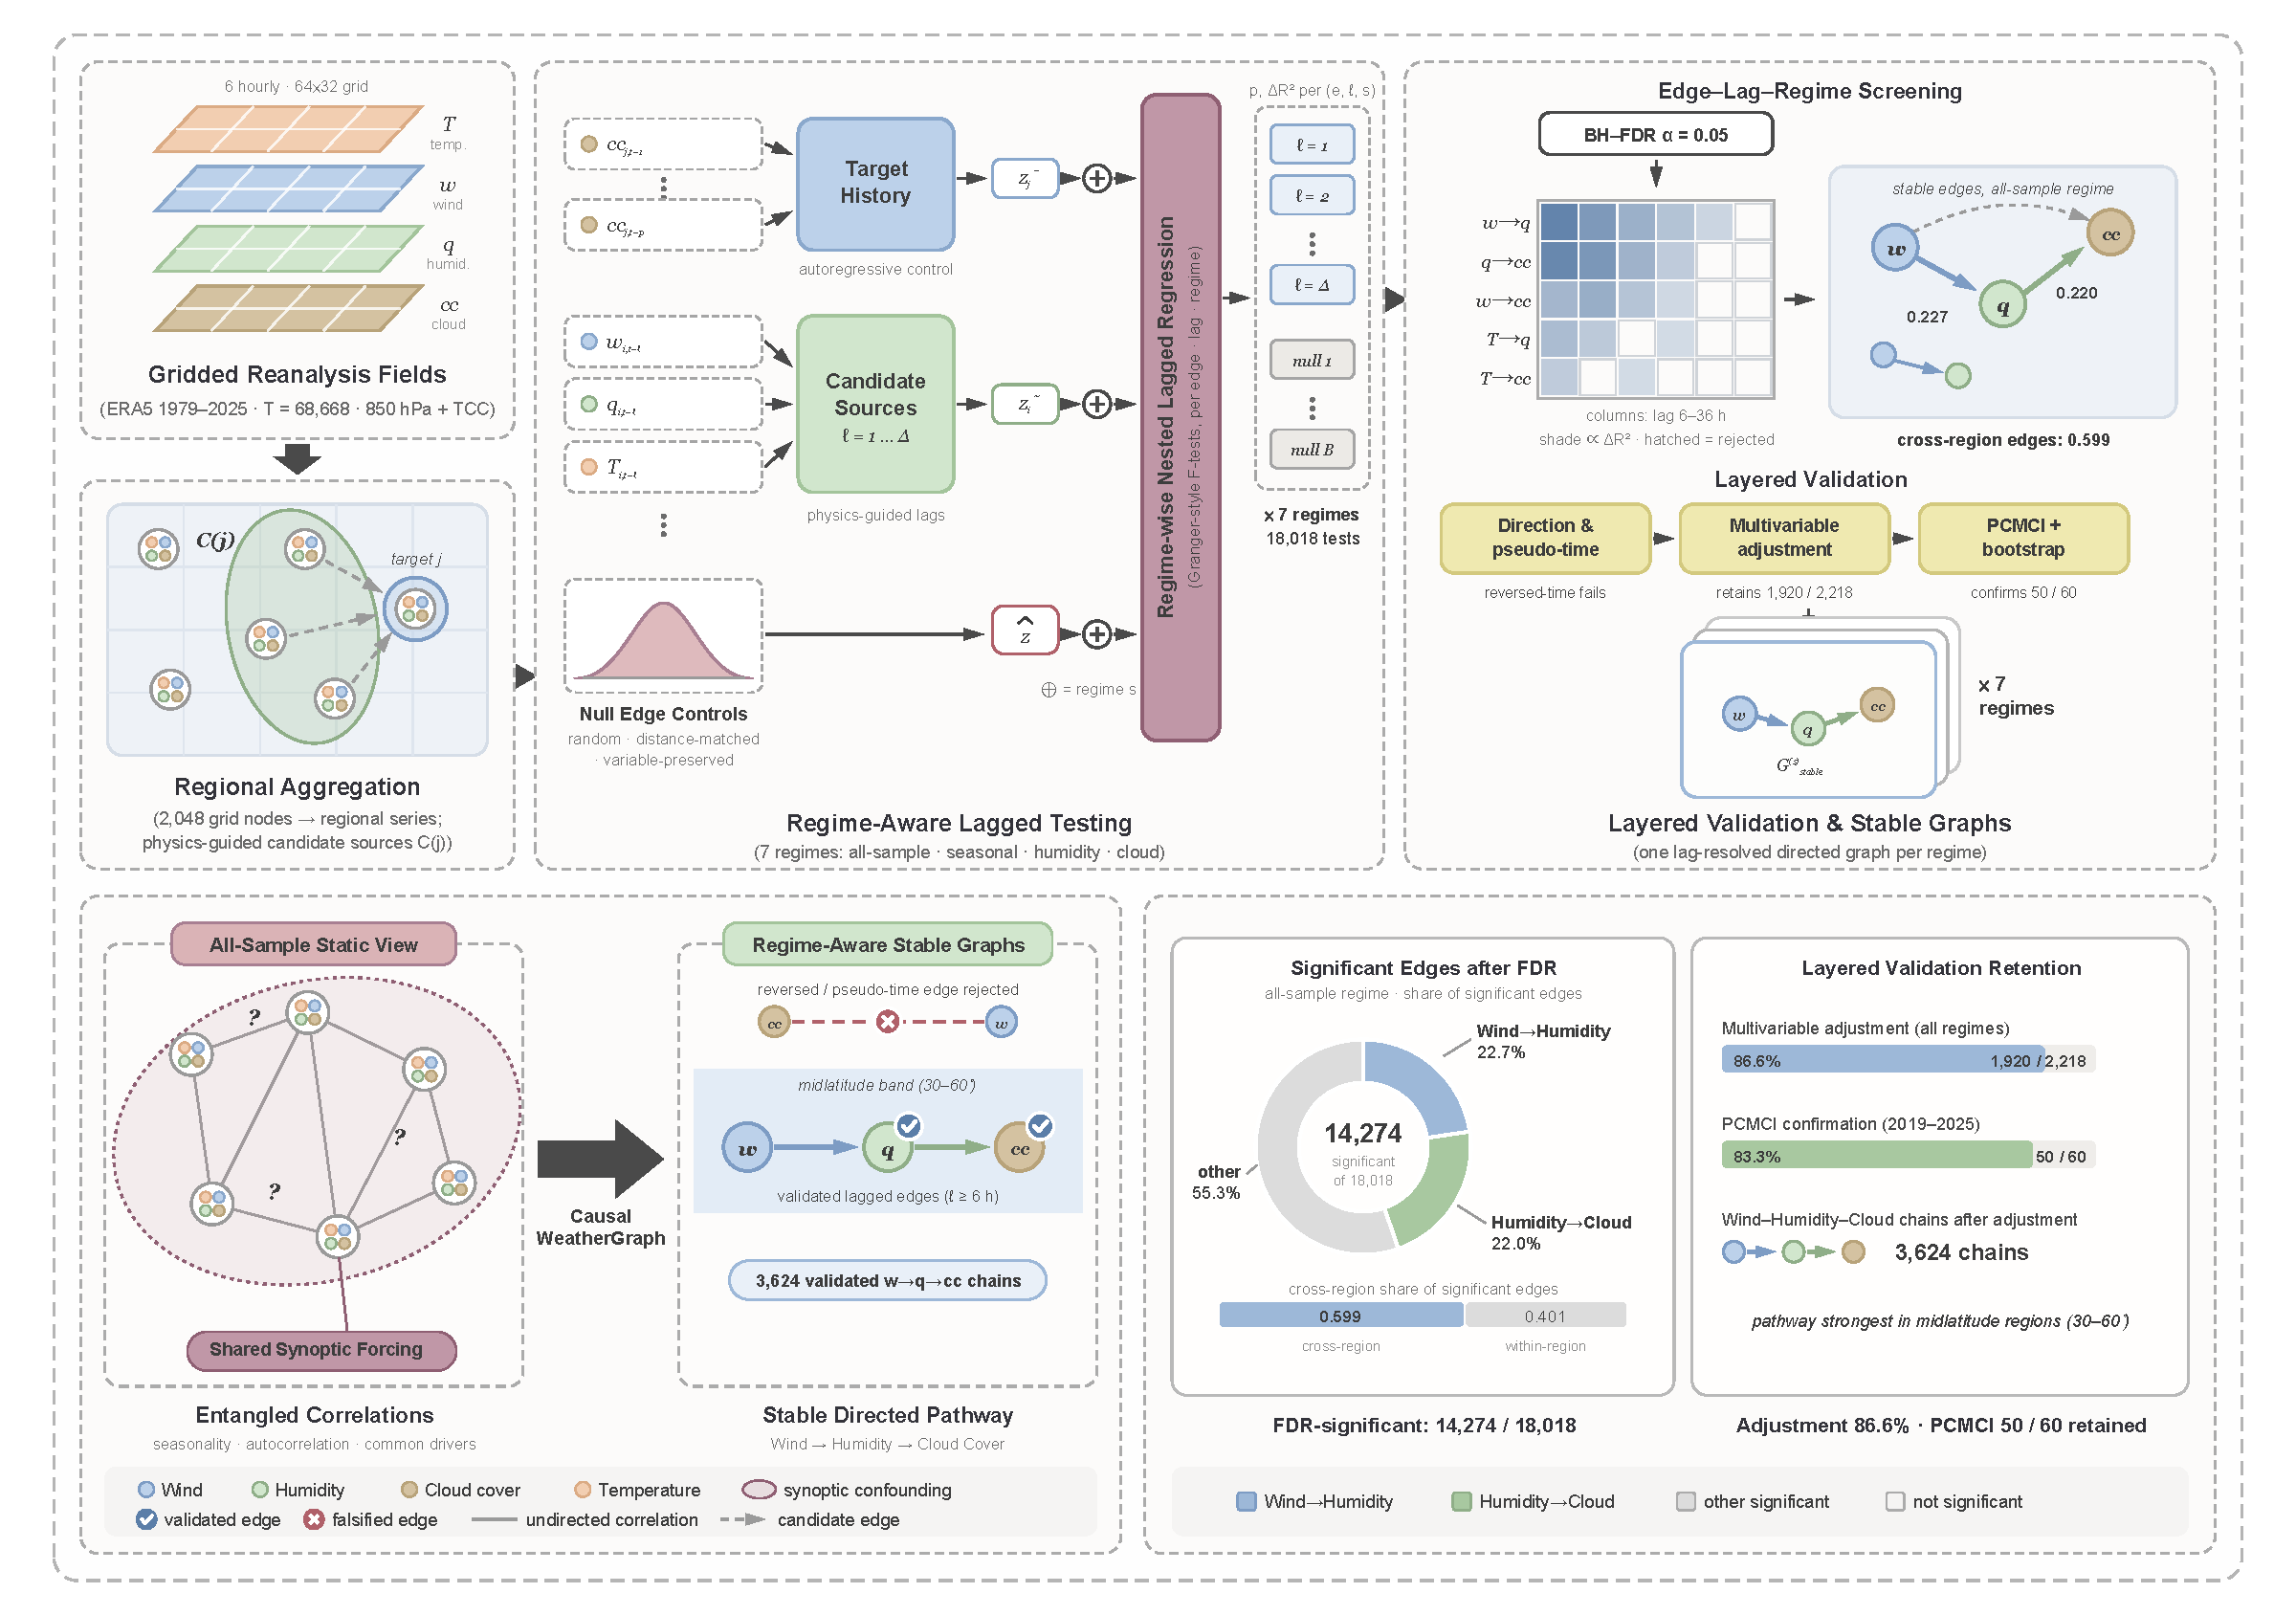
\includegraphics[width=0.98\textwidth]{figures/framework/fig_framework_causal_weathergraph_editable.pdf}
}\DIFdelendFL \DIFaddbeginFL \DIFaddFL{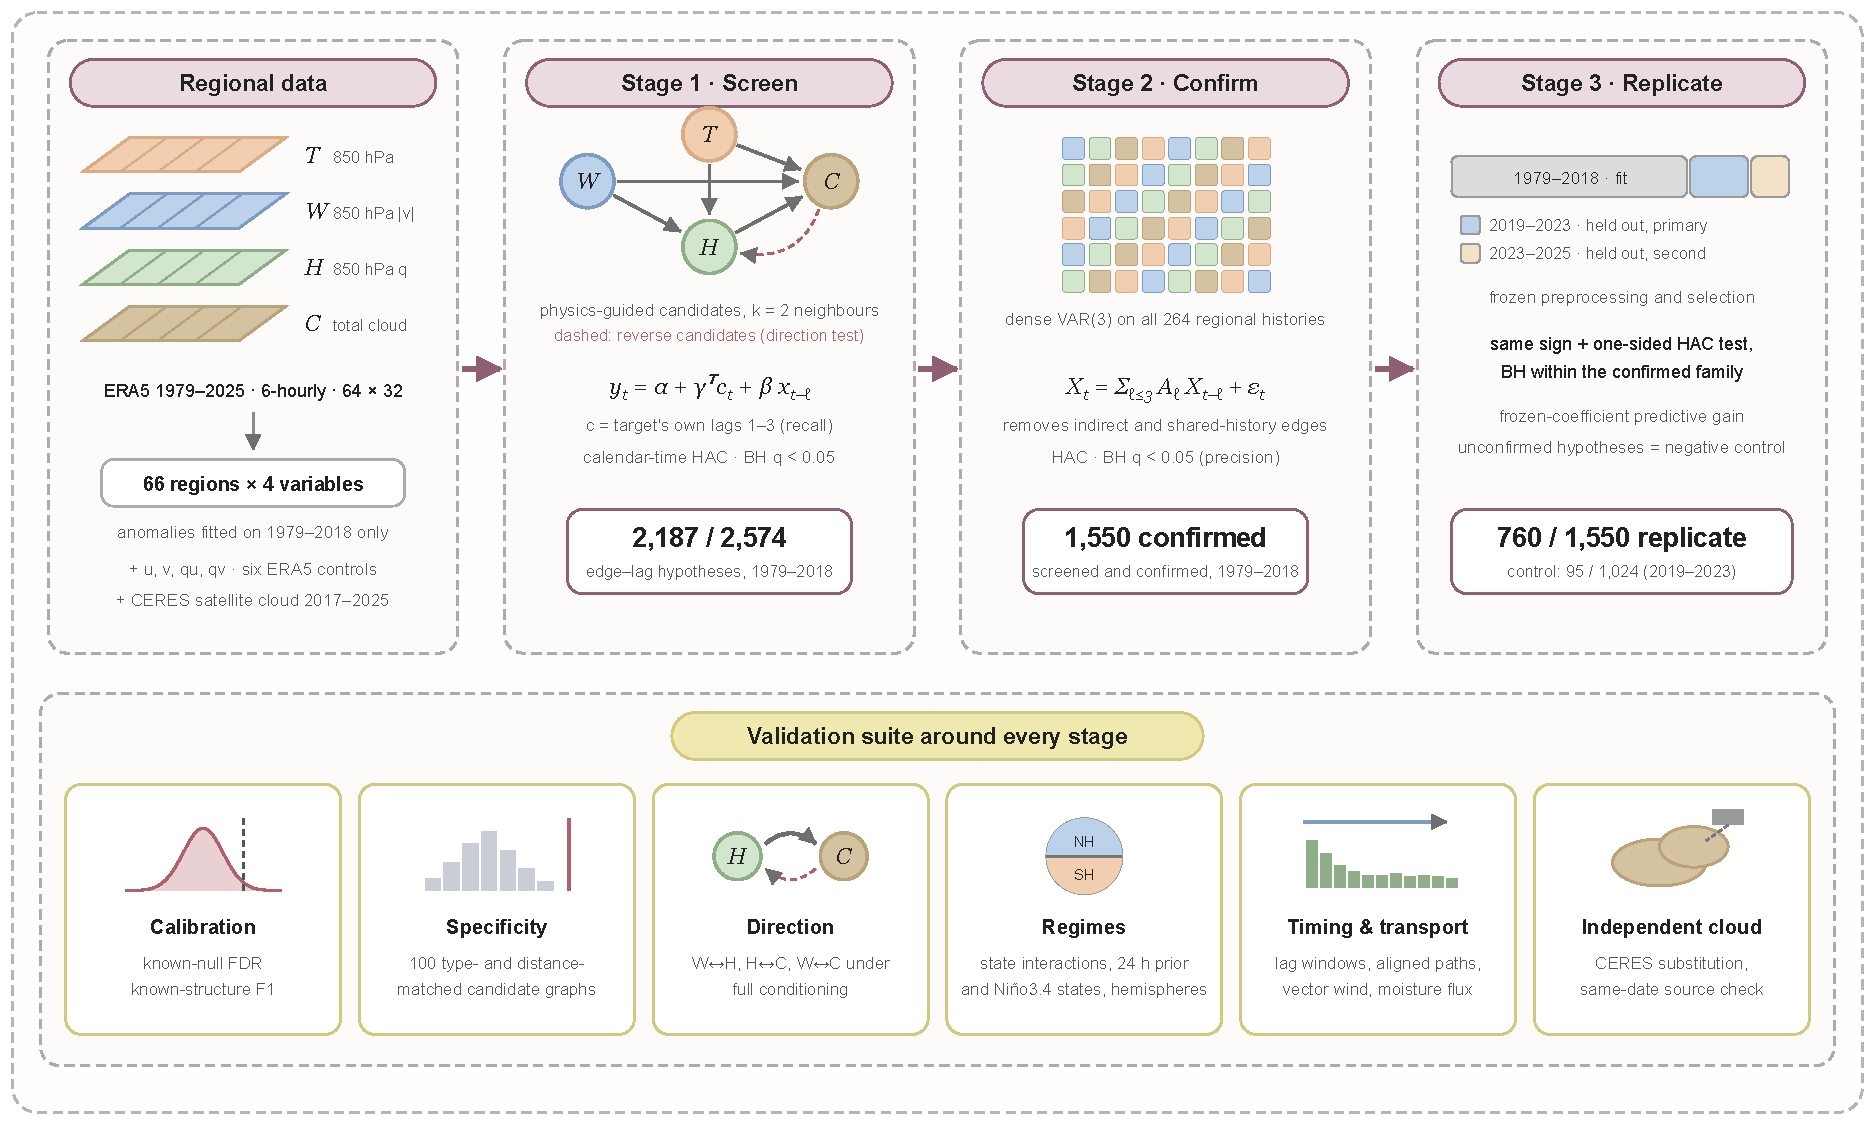
\includegraphics[width=0.98\textwidth]{figures/fig01_framework.pdf}
}\DIFaddendFL \caption{Overview of \DIFdelbeginFL \DIFdelFL{the }\DIFdelendFL Causal WeatherGraph\DIFdelbeginFL \DIFdelFL{framework and headline results}\DIFdelendFL . \DIFdelbeginFL \DIFdelFL{ERA5 fields (1979--2025) }\DIFdelendFL \DIFaddbeginFL \DIFaddFL{Physics-guided candidates }\DIFaddendFL are \DIFdelbeginFL \DIFdelFL{aggregated into regional multivariate series, constrained by physics-guided candidate edges, and }\DIFdelendFL screened \DIFdelbeginFL \DIFdelFL{by regime-wise nested lagged regressions }\DIFdelendFL with \DIFdelbeginFL \DIFdelFL{BH--FDR control }\DIFdelendFL \DIFaddbeginFL \DIFaddFL{own-history regressions, confirmed under full conditioning }\DIFaddendFL and \DIFaddbeginFL \DIFaddFL{replicated in held-out years, while }\DIFaddendFL a \DIFdelbeginFL \DIFdelFL{layered }\DIFdelendFL validation \DIFdelbeginFL \DIFdelFL{chain; 14}\DIFdelendFL \DIFaddbeginFL \DIFaddFL{suite tests calibration}\DIFaddendFL , \DIFdelbeginFL \DIFdelFL{274 of 18}\DIFdelendFL \DIFaddbeginFL \DIFaddFL{specificity}\DIFaddendFL , \DIFdelbeginFL \DIFdelFL{018 (edge}\DIFdelendFL \DIFaddbeginFL \DIFaddFL{direction}\DIFaddendFL , \DIFdelbeginFL \DIFdelFL{lag, }\DIFdelendFL regime \DIFdelbeginFL \DIFdelFL{) tests remain significant}\DIFdelendFL \DIFaddbeginFL \DIFaddFL{dependence}\DIFaddendFL , \DIFdelbeginFL \DIFdelFL{dominated by Wind $\rightarrow$ Humidity }\DIFdelendFL \DIFaddbeginFL \DIFaddFL{timing }\DIFaddendFL and \DIFdelbeginFL \DIFdelFL{Humidity $\rightarrow$ Cloud Cover}\DIFdelendFL \DIFaddbeginFL \DIFaddFL{product dependence}\DIFaddendFL .}
\label{fig:framework}
\end{figure}

We make \DIFdelbegin \DIFdel{three }\DIFdelend \DIFaddbegin \DIFadd{four }\DIFaddend main contributions:
\begin{itemize}
\item \textbf{\DIFdelbegin \DIFdel{Scalable physics-constrained graph construction}\DIFdelend \DIFaddbegin \DIFadd{A screen--confirm--replicate framework}\DIFaddend .} We \DIFdelbegin \DIFdel{compress high-dimensional gridded fields into interpretable region--variable nodes and restrict the edge hypothesis space to physically admissible candidates, reducing an intractable unconstrained search to 18, 018 regime-conditioned lagged tests while preserving physical interpretability and computational feasibility.
}%DIFDELCMD < \item %%%
\item%DIFAUXCMD
\textbf{\DIFdel{Regime-aware structure estimation.}} %DIFAUXCMD
\DIFdel{We estimate separate graph structures for the all-sample, seasonal, high-humidity, normal-humidity, high-cloud and normal-cloud regimes rather than forcing all samples into a single static graph, making state-dependent dependency structure an explicit object of analysis}\DIFdelend \DIFaddbegin \DIFadd{separate recall-oriented screening of physics-guided candidates, confirmation under full conditioning on all observed regional histories, and held-out replication with a negative control, so that replicable dependencies are distinguished from shared-history, indirect and spatial-background artefacts in large spatio-temporal records}\DIFaddend .
\item \textbf{\DIFdelbegin \DIFdel{Layered statistical validation}\DIFdelend \DIFaddbegin \DIFadd{Calibration and benchmarking}\DIFaddend .} We \DIFdelbegin \DIFdel{couple the discovery step with a reusable validation chain --- random, distance-matched and variable-preserved edge controls; directionality and pseudo-time falsification; target-region multivariable adjustment; effect-size and confidence-interval reporting; PCMCIconfirmation; block bootstrap; long-lag and humidity-mediation tests; latitude-band stratification; matched-sample regime analysis; candidate-$k$ expansion; historical-period stability; and preprocessing and region-aggregation robustness --- so that the reported structure is explicitly controlled for the dependence artefacts that observational spatio-temporal data induce.
}\DIFdelend \DIFaddbegin \DIFadd{calibrate each stage with known-null and known-structure simulations and compare it with multivariable Granger regression, PCMCI, Regime-PCMCI and CaStLe under matched information, together with runtime and memory measurements, showing that single-stage own-history screening is reliable only for weakly coupled systems.
}\item \textbf{\DIFadd{A replicable wind--humidity--cloud dependency set.}} \DIFadd{We apply the framework to 47 years of ERA5 and to CERES satellite cloud, identify 760 replicated conditional dependencies, and show which pathway properties survive, notably a modest humidity$\rightarrow$cloud asymmetry, and which do not, namely chain enrichment, window-free interpretation of path lags, uniform winter strengthening and cloud-state regimes.
}\item \textbf{\DIFadd{A pre-specified eddy predictor of cloud.}} \DIFadd{We decompose the 850-hPa moisture flux exactly into climatological, linear and quadratic parts, define a regional wind--humidity eddy convergence (WHEC) from the quadratic part, and show in a test frozen before any result that it reduces held-out cloud-prediction error beyond the dense autoregression and linear transport terms, with midlatitude gains 2.5--3.1 times the tropical gains, whereas remote-region and time-shifted versions add nothing.
}\DIFaddend \end{itemize}

\section{Related Work}
\label{sec:related}

\DIFdelbegin \DIFdel{Figure~2 situates Causal WeatherGraph within four strands of related research: data-driven atmospheric prediction, spatio-temporal graph and multivariate time-series learning, causal discovery for Earth-system time series, and regime-dependent atmospheric interactions.
}\DIFdelend \DIFaddbegin \subsection{\DIFadd{Data-driven atmospheric prediction and learned graphs}}

\DIFaddend 

\DIFdelbegin %DIFDELCMD < \begin{figure}[htbp]
%DIFDELCMD < \centering
%DIFDELCMD < %%%
\DIFdelFL{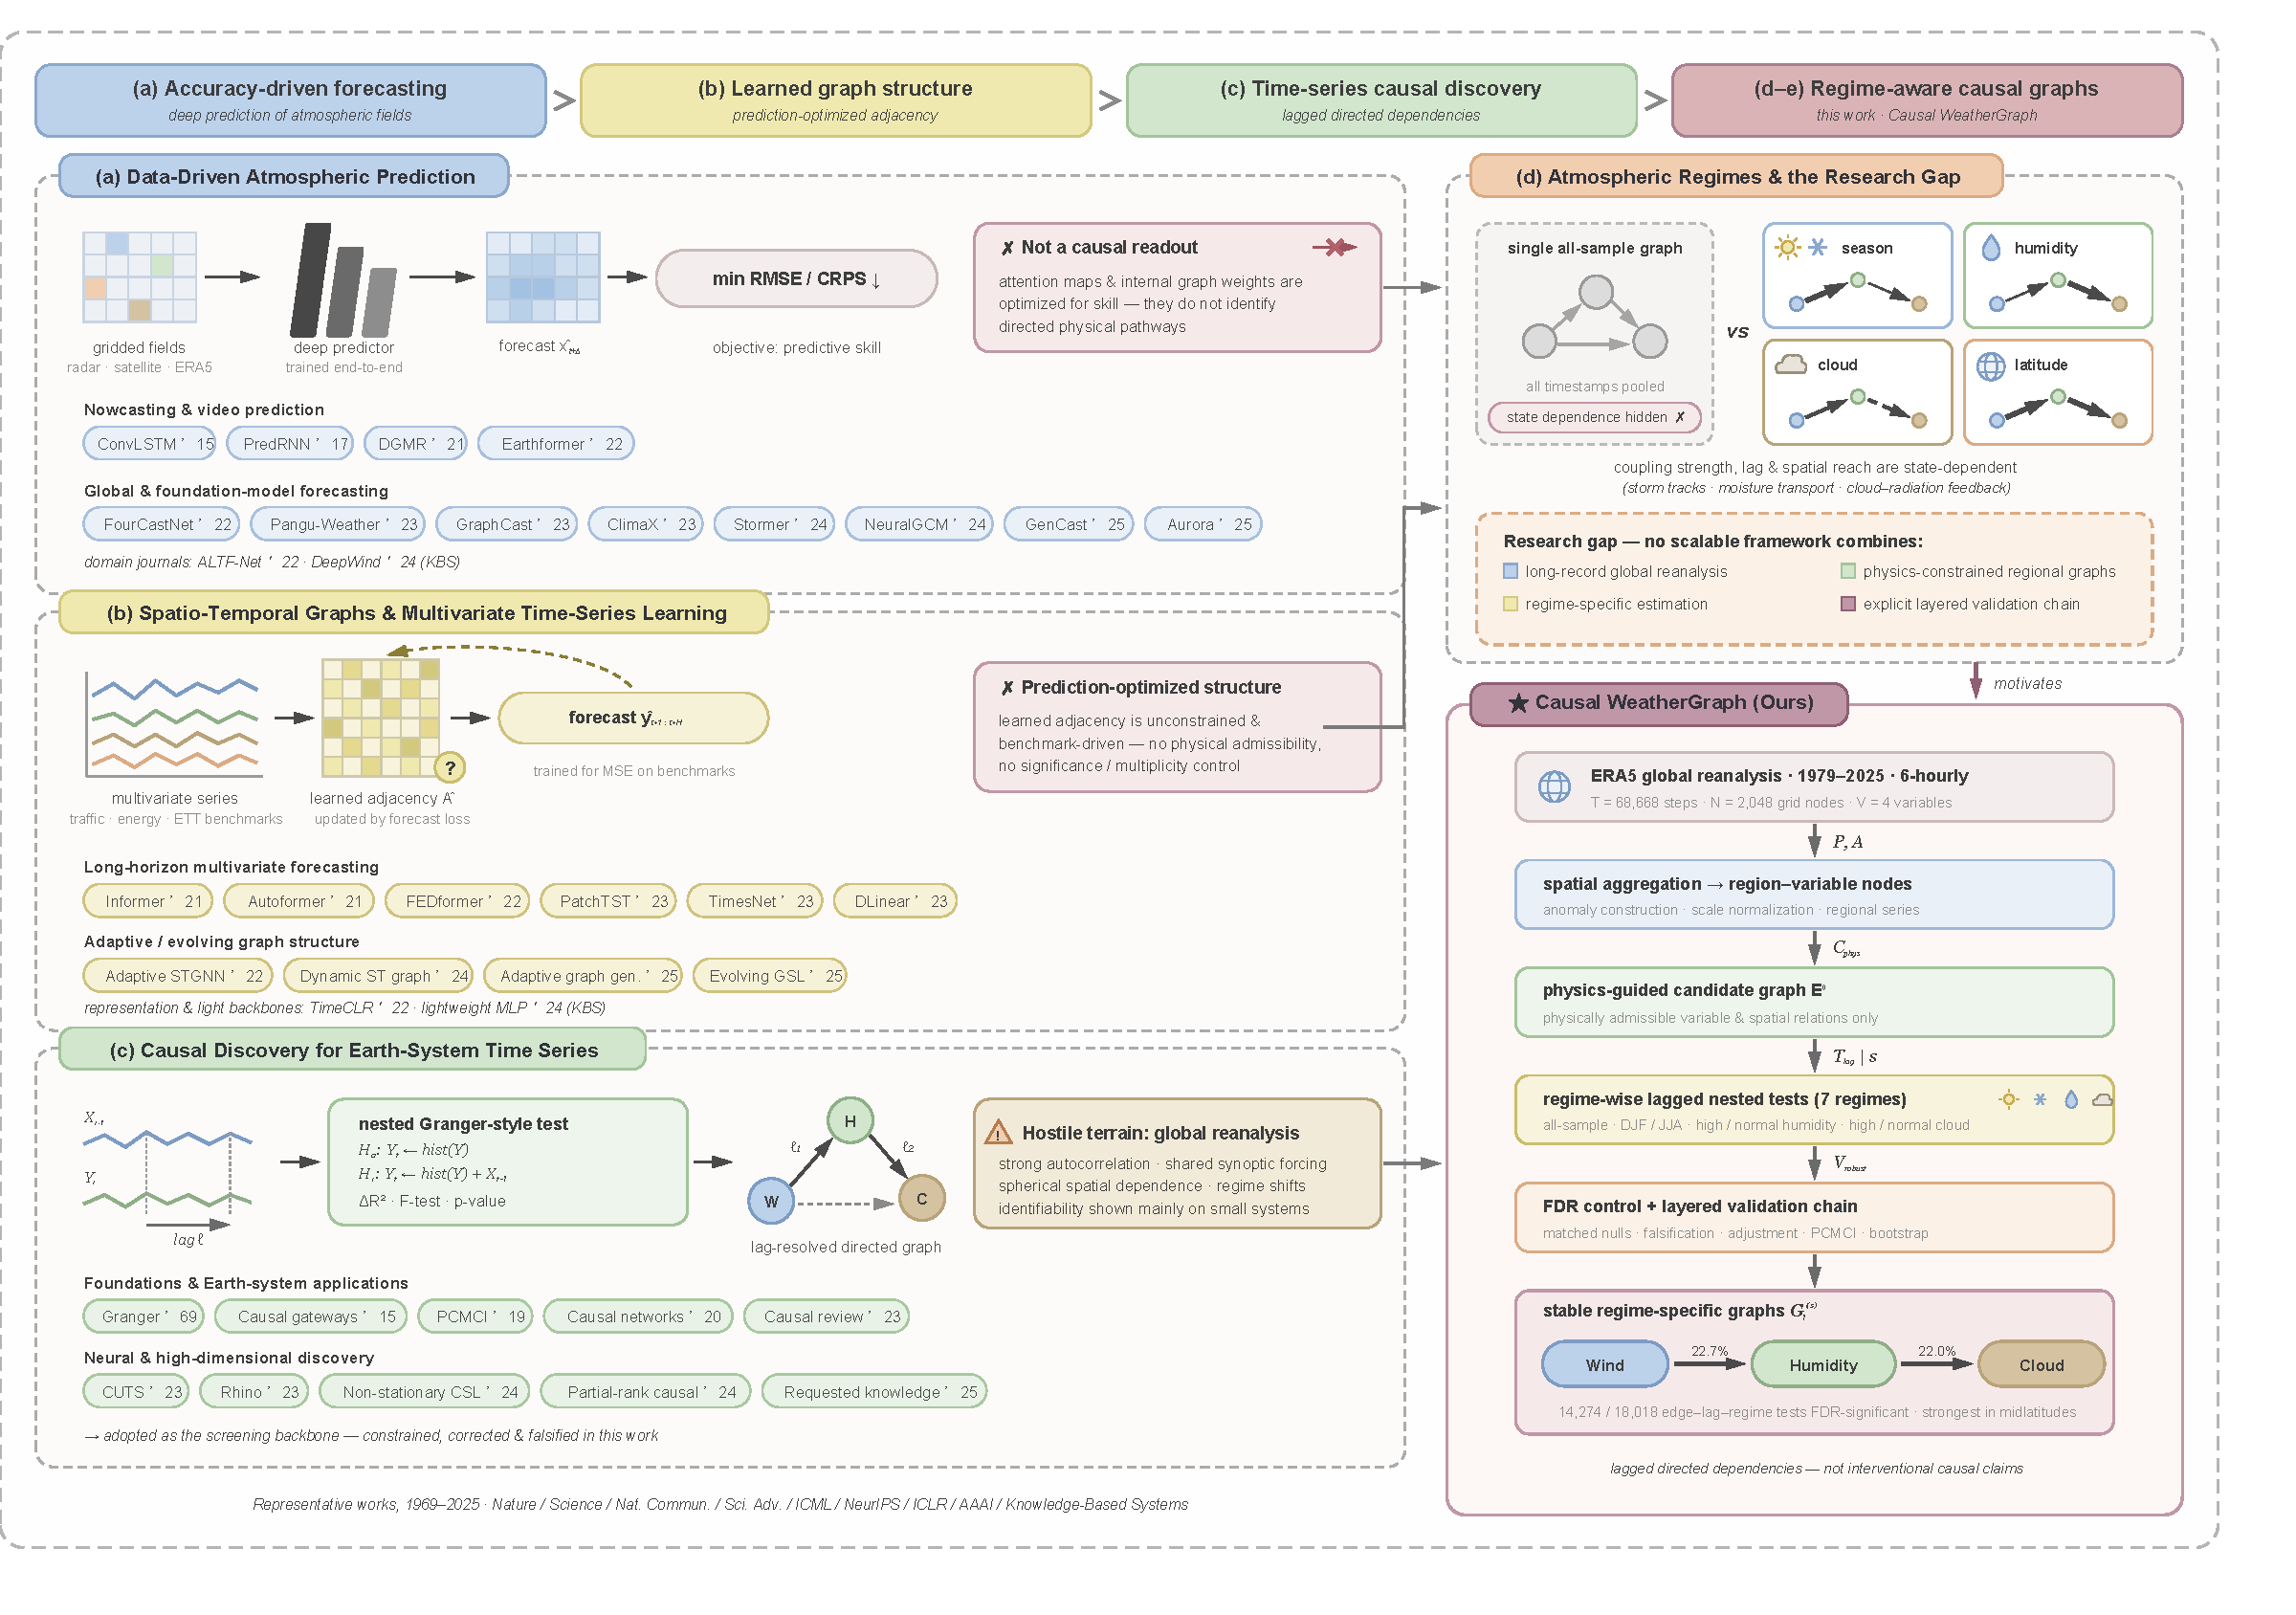
\includegraphics[width=0.98\textwidth]{figures/related_work/fig_related_work_causal_weathergraph_editable.pdf}
}%DIFDELCMD < \caption{%
{%DIFAUXCMD
\DIFdelFL{Positioning of Causal WeatherGraph within related work. Predictive models (a--b) optimize forecast skill rather than directed physical pathways, causal discovery (c) is strained by the dependence structure of global reanalysis, and single all-sample graphs (d) obscure regime differences; Causal WeatherGraph (e) closes this gap with physics-guided candidates, regime-wise lagged tests and layered validation.}}
%DIFAUXCMD
%DIFDELCMD < \label{fig:related-work}
%DIFDELCMD < \end{figure}
%DIFDELCMD < 

%DIFDELCMD < %%%
\subsection{\DIFdel{Data-driven atmospheric prediction}}
%DIFAUXCMD
\addtocounter{subsection}{-1}%DIFAUXCMD
%DIFDELCMD < 

%DIFDELCMD < %%%
\DIFdel{Deep spatio-temporal prediction established that neural networks can learn nonlinear evolution from radar, satellite and reanalysis fields. ConvLSTM and PredRNN introduced convolutional recurrent memory for precipitation nowcasting and predictive learning \mbox{%DIFAUXCMD
\citep{Shi2015ConvLSTM,Wang2017PredRNN}}\hskip0pt%DIFAUXCMD
; more recent systems use generative modelling and space--time attention to improve probabilistic nowcasting and long-range dependence representation \mbox{%DIFAUXCMD
\citep{Ravuri2021Nowcasting,Gao2022Earthformer}}\hskip0pt%DIFAUXCMD
. Recent work has also moved toward transferable atmospheric representations: ClimaX formulates weather and climate modelling as a foundation-model problem \mbox{%DIFAUXCMD
\citep{Nguyen2023ClimaX}}\hskip0pt%DIFAUXCMD
, while Stormer studies the scaling of transformer weather models \mbox{%DIFAUXCMD
\citep{Nguyen2024Stormer}}\hskip0pt%DIFAUXCMD
.
In the applied forecasting literature, ALTF-Net applies attention to long-horizon air-temperature forecasting, while DeepWind combines heterogeneous spatial and temporal information for wind forecasting \mbox{%DIFAUXCMD
\citep{Nandi2022ALTF,Wang2024DeepWind}}\hskip0pt%DIFAUXCMD
. These studies demonstrate the value of learned multiscale representations for atmospheric series, but their primary objective is predictive accuracy rather than the identification and falsification of interpretable directed physical pathways.
}%DIFDELCMD < 

%DIFDELCMD < %%%
\DIFdelend Global data-driven forecasting has \DIFdelbegin \DIFdel{advanced from Fourier }\DIFdelend \DIFaddbegin \DIFadd{progressed from }\DIFaddend neural operators and three-dimensional \DIFdelbegin \DIFdel{neural architectures }\DIFdelend \DIFaddbegin \DIFadd{networks }\DIFaddend to graph-based, hybrid \DIFdelbegin \DIFdel{dynamical and probabilistic ensemble systems. FourCastNet, }\DIFdelend \DIFaddbegin \DIFadd{and probabilistic systems. GraphCast \mbox{%DIFAUXCMD
\citep{Lam2023GraphCast} }\hskip0pt%DIFAUXCMD
and }\DIFaddend Pangu-Weather \DIFdelbegin \DIFdel{and GraphCast established competitive }\DIFdelend \DIFaddbegin \DIFadd{\mbox{%DIFAUXCMD
\citep{Bi2023Pangu} }\hskip0pt%DIFAUXCMD
established }\DIFaddend medium-range \DIFdelbegin \DIFdel{global forecasting \mbox{%DIFAUXCMD
\citep{Pathak2022FourCastNet,Bi2023Pangu,Lam2023GraphCast}}\hskip0pt%DIFAUXCMD
; WeatherBench~2 subsequently provided a standardized evaluation framework \mbox{%DIFAUXCMD
\citep{Rasp2024WeatherBench2}}\hskip0pt%DIFAUXCMD
. NeuralGCM couples machine-learned }\DIFdelend \DIFaddbegin \DIFadd{skill comparable with operational systems, NeuralGCM couples learned }\DIFaddend components with a differentiable \DIFdelbegin \DIFdel{atmospheric dynamical core , GenCast extends global prediction to probabilistic ensembles , and Aurora demonstrates a foundation model spanning multiple Earth-system forecasting tasks \mbox{%DIFAUXCMD
\citep{Kochkov2024NeuralGCM,Price2025GenCast,Bodnar2025Aurora}}\hskip0pt%DIFAUXCMD
. Collectively, this recent literature shows that atmospheric states are naturally modelled through multiscale spatial interactions. Nevertheless, the internal graph or attention weights of a forecasting model are optimized for prediction and should not automatically be interpreted as causal or physically directed edges.
}%DIFDELCMD < 

%DIFDELCMD < %%%
\subsection{\DIFdel{Spatio-temporal graphs and multivariate time-series learning}}
%DIFAUXCMD
\addtocounter{subsection}{-1}%DIFAUXCMD
%DIFDELCMD < 

%DIFDELCMD < %%%
\DIFdel{Long-horizon multivariate forecasting has evolved rapidly. Informer introduced efficient attention for long sequences, Autoformer incorporated decomposition and autocorrelation, and FEDformer used frequency-enhanced decomposition \mbox{%DIFAUXCMD
\citep{Zhou2021Informer,Wu2021Autoformer,Zhou2022FEDformer}}\hskip0pt%DIFAUXCMD
. PatchTST and TimesNet subsequently developed patch-based channel modelling and multi-period two-dimensional temporal representations, while DLinear showed that carefully designed linear baselines remain highly competitive \mbox{%DIFAUXCMD
\citep{Nie2023PatchTST,Wu2023TimesNet,Zeng2023DLinear}}\hskip0pt%DIFAUXCMD
. This body of work motivates careful separation between representational complexity and scientifically interpretable dependence.
}%DIFDELCMD < 

%DIFDELCMD < %%%
\DIFdel{Recent spatio-temporal graph research increasingly learns or updates graph topology instead of assuming a fixed adjacency matrix. Adaptive graph neural networks, dynamic spatial-aware graph transformers and unified adaptive graph-generation methods have improved forecasting where spatial relations change over time \mbox{%DIFAUXCMD
\citep{Ta2022AdaptiveSTGNN,Li2024DynamicGraph,Wang2025AdaptiveGraph}}\hskip0pt%DIFAUXCMD
. Evolving graph structure learning further links changing multivariate dependencies to forecasting performance \mbox{%DIFAUXCMD
\citep{Ye2025EvolvingGraph}}\hskip0pt%DIFAUXCMD
.

In weather forecasting specifically, HiSTGNN learns a hierarchical graph that couples a }\DIFdelend \DIFaddbegin \DIFadd{dynamical core \mbox{%DIFAUXCMD
\citep{Kochkov2024NeuralGCM}}\hskip0pt%DIFAUXCMD
, and GenCast generates probabilistic ensembles \mbox{%DIFAUXCMD
\citep{Price2025GenCast}}\hskip0pt%DIFAUXCMD
. Spatio-temporal graph neural networks learn adjacency jointly with forecasts, for example hierarchical graphs that link }\DIFaddend station-level \DIFdelbegin \DIFdel{global graph with }\DIFdelend \DIFaddbegin \DIFadd{and }\DIFaddend variable-level \DIFdelbegin \DIFdel{local graphs and passes information bidirectionally between the two levels, improving multi-station}\DIFdelend \DIFaddbegin \DIFadd{structure for weather prediction \mbox{%DIFAUXCMD
\citep{Ma2023HiSTGNN} }\hskip0pt%DIFAUXCMD
and evolving graph structures for multivariate series \mbox{%DIFAUXCMD
\citep{Ye2025EvolvingGraph}}\hskip0pt%DIFAUXCMD
, whereas carefully specified linear models remain strong multivariate forecasting baselines \mbox{%DIFAUXCMD
\citep{Zeng2023DLinear}}\hskip0pt%DIFAUXCMD
. These models minimize predictive loss. Their attention weights and learned adjacencies are not tested hypotheses about directed lagged dependence}\DIFaddend , \DIFdelbegin \DIFdel{multi-variable prediction \mbox{%DIFAUXCMD
\citep{Ma2023HiSTGNN}}\hskip0pt%DIFAUXCMD
. Complementary work develops self-supervised time-series representations and lightweight multivariate forecasting backbones \mbox{%DIFAUXCMD
\citep{Yang2022TimeCLR,Wang2024LightweightMLP}}\hskip0pt%DIFAUXCMD
. Although most of these methods were evaluated on traffic, industrial or generic benchmark series, they provide relevant computational ideas for large spatio-temporal systems. The distinction is that Causal WeatherGraph does not learn an unconstrained predictive adjacency: it begins from physically admissible variable and spatial relations, estimates explicit positive-lag tests, applies multiplicity control, and reports graph edges only within a layered falsification framework.
}\DIFdelend \DIFaddbegin \DIFadd{and none of them controls or verifies the error rate of the structure it implies.

}\DIFaddend 

\subsection{Causal discovery for Earth-system time series}

\DIFdelbegin \DIFdel{Granger causality formalized temporal precedence and incremental prediction for lagged time series \mbox{%DIFAUXCMD
\citep{Granger1969}}\hskip0pt%DIFAUXCMD
}\DIFdelend \DIFaddbegin \DIFadd{Granger's criterion asks whether the history of a source improves the prediction of a target given a stated information set; its multivariable form conditions on all observed histories in a vector autoregression, and recent extensions address high-dimensional, nonlinear and subsampled series \mbox{%DIFAUXCMD
\citep{Shojaie2022Granger}}\hskip0pt%DIFAUXCMD
}\DIFaddend . Earth-system \DIFdelbegin \DIFdel{causal discovery subsequently combined }\DIFdelend \DIFaddbegin \DIFadd{applications combine this idea with }\DIFaddend conditional-independence testing \DIFdelbegin \DIFdel{, graphical models and domain constraints to identify gateways, mediators and model-process relationships \mbox{%DIFAUXCMD
\citep{Runge2015Gateways,Runge2019Causation,Nowack2020CausalNetworks}}\hskip0pt%DIFAUXCMD
. A recent cross-disciplinary review emphasizes that causal discovery from observational dynamical systems requires explicit assumptions about temporal order, hidden confounding, non-stationarity and functional form \mbox{%DIFAUXCMD
\citep{CampsValls2023CausalRelations}}\hskip0pt%DIFAUXCMD
. CUTS extended neural causal discovery to irregularly sampled time series, while Rhino modelled temporal causal relations with }\DIFdelend \DIFaddbegin \DIFadd{and domain knowledge \mbox{%DIFAUXCMD
\citep{Runge2023TimeSeries}}\hskip0pt%DIFAUXCMD
, and causal-network analyses of teleconnections state the assumed pathways and information sets explicitly before quantifying them \mbox{%DIFAUXCMD
\citep{Kretschmer2021Pathways}}\hskip0pt%DIFAUXCMD
. PCMCI selects conditioning sets with a PC-type stage before testing momentary conditional independence and was designed for large nonlinear systems \mbox{%DIFAUXCMD
\citep{Runge2019PCMCI}}\hskip0pt%DIFAUXCMD
. Neural methods address irregular sampling \mbox{%DIFAUXCMD
\citep{Cheng2023CUTS} }\hskip0pt%DIFAUXCMD
and }\DIFaddend history-dependent \DIFdelbegin \DIFdel{noise \mbox{%DIFAUXCMD
\citep{Cheng2023CUTS,Gong2023Rhino}}\hskip0pt%DIFAUXCMD
. Recent studies additionally address }\DIFdelend \DIFaddbegin \DIFadd{noise \mbox{%DIFAUXCMD
\citep{Gong2023Rhino}}\hskip0pt%DIFAUXCMD
, structure learning has been extended to }\DIFaddend high-dimensional non-stationary \DIFdelbegin \DIFdel{causal structure learning , partial-rank-correlation causal networks and the use of dynamically requested background knowledge \mbox{%DIFAUXCMD
\citep{Chen2024NonstationaryCausal,Yang2024PartialRankCausal,Kitson2025RequestedKnowledge}}\hskip0pt%DIFAUXCMD
. These developments are closely related to the present objective, but global atmospheric reanalysis introduces unusually strong autocorrelation, shared synoptic forcing, spherical spatial dependence and regime shifts. We therefore use scalable Granger-style nested regression as the screening backbone and constrain its interpretation through physics-guided candidates, false-discovery control, temporal falsification, multivariable adjustment, PCMCI confirmation and robustness analysis.
}\DIFdelend \DIFaddbegin \DIFadd{series \mbox{%DIFAUXCMD
\citep{Chen2024NonstationaryCausal}}\hskip0pt%DIFAUXCMD
, and background knowledge can be requested dynamically to constrain the search \mbox{%DIFAUXCMD
\citep{Kitson2025RequestedKnowledge}}\hskip0pt%DIFAUXCMD
. Comparisons on synthetic systems and climate indices show that causal methods outperform correlation analysis but can disagree with one another \mbox{%DIFAUXCMD
\citep{Docquier2024Comparison}}\hskip0pt%DIFAUXCMD
, and benchmarks generated from real series with known graphs have been proposed to evaluate such methods \mbox{%DIFAUXCMD
\citep{Cheng2024CausalTime}}\hskip0pt%DIFAUXCMD
. Two approaches are closest to our setting. Regime-PCMCI learns persistent hidden regimes jointly with regime-specific causal graphs \mbox{%DIFAUXCMD
\citep{Saggioro2020RegimePCMCI}}\hskip0pt%DIFAUXCMD
, and CaStLe exploits local space--time stencils and spatial homogeneity to discover structure on gridded fields \mbox{%DIFAUXCMD
\citep{Nichol2025CaStLe}}\hskip0pt%DIFAUXCMD
. Both target identification under explicit assumptions on comparatively small or spatially homogeneous systems. Neither is designed to verify whether a large, nearly saturated discovered graph replicates out of sample, which is the gap that our framework addresses (Table~\ref{tab:positioning}).

}\DIFaddend 

\DIFaddbegin \begin{table}[htbp]
\centering
\caption{\DIFaddFL{Positioning of Causal WeatherGraph relative to related approaches.}}
\label{tab:positioning}
\footnotesize
\setlength{\tabcolsep}{3pt}
\begin{tabular}{@{}p{0.16\textwidth}p{0.17\textwidth}p{0.17\textwidth}p{0.20\textwidth}p{0.235\textwidth}@{}}
\toprule
\DIFaddFL{Approach }& \DIFaddFL{Candidate space }& \DIFaddFL{Conditioning }& \DIFaddFL{Regimes and space }& \DIFaddFL{Verification of the graph }\\
\midrule
\DIFaddFL{Multivariable Granger \mbox{%DIFAUXCMD
\citep{Shojaie2022Granger} }\hskip0pt%DIFAUXCMD
}& \DIFaddFL{All pairs }& \DIFaddFL{All observed lags }& \DIFaddFL{None }& \DIFaddFL{In-sample tests }\\
\DIFaddFL{PCMCI \mbox{%DIFAUXCMD
\citep{Runge2019PCMCI} }\hskip0pt%DIFAUXCMD
}& \DIFaddFL{All pairs or assumed links }& \DIFaddFL{PC-selected parents }& \DIFaddFL{None }& \DIFaddFL{In-sample tests }\\
\DIFaddFL{Regime-PCMCI \mbox{%DIFAUXCMD
\citep{Saggioro2020RegimePCMCI} }\hskip0pt%DIFAUXCMD
}& \DIFaddFL{All pairs or assumed links }& \DIFaddFL{PC-selected parents per regime }& \DIFaddFL{Learned hidden persistent regimes }& \DIFaddFL{In-sample tests }\\
\DIFaddFL{CaStLe \mbox{%DIFAUXCMD
\citep{Nichol2025CaStLe} }\hskip0pt%DIFAUXCMD
}& \DIFaddFL{Local stencil neighbours }& \DIFaddFL{Stencil parents }& \DIFaddFL{Shared local stencil on a grid }& \DIFaddFL{In-sample tests }\\
\DIFaddFL{Causal WeatherGraph (this work) }& \DIFaddFL{Physics-guided set plus symmetric reverse set }& \DIFaddFL{Own history (screen); all 264 regional histories (confirm) }& \DIFaddFL{Prescribed, antecedent and external states with interaction tests; distance-matched null graphs }& \DIFaddFL{Held-out replication, frozen predictive gain, negative control, satellite substitution }\\
\bottomrule
\end{tabular}
\end{table}

\DIFaddend \subsection{Atmospheric regimes\DIFaddbegin \DIFadd{, cloud-controlling factors }\DIFaddend and \DIFdelbegin \DIFdel{the research gap}\DIFdelend \DIFaddbegin \DIFadd{reanalysis}\DIFaddend }

\DIFdelbegin \DIFdel{Atmospheric interactions are state dependent. Season, humidity background, cloud regime and latitude-band distribution can alter coupling strength, lag and spatial reach. Synoptic-scale circulation organizes moisture transport in midlatitude cyclones, while storm tracks interact with water vapour, latent heating, clouds and radiation \mbox{%DIFAUXCMD
\citep{Boutle2011Moisture,Shaw2016StormTracks,Ceppi2015Clouds}}\hskip0pt%DIFAUXCMD
. Consequently, a single graph estimated from all timestamps may obscure physically meaningful changes in pathway prevalence or strength. Existing forecasting studies usually assess skill by lead time and variable, whereas causal-discovery studies often prioritize methodological identifiability on smaller systems. The unresolved gap is a scalable framework that combines long-record global reanalysis, physically constrained regional graphs, regime-specific estimation and an explicit validation chain. Causal WeatherGraph addresses this gap by comparing pathway counts, edge-type fractions, cross-region fractions, lags, chain scores and stability across seasonal, humidity and cloud regimes. }\DIFdelend \DIFaddbegin \DIFadd{Extratropical clouds are organized by the large-scale circulation and hydrological cycle; across climate models, the sensitivity of Southern Ocean cloud liquid water to moisture convergence helps predict the shortwave cloud feedback \mbox{%DIFAUXCMD
\citep{McCoy2022Extratropical}}\hskip0pt%DIFAUXCMD
. Cloud-controlling-factor analyses relate cloud and cloud-radiative anomalies to large-scale humidity, stability, vertical motion and advection, for example with regularized regressions fitted to two decades of near-global satellite and reanalysis data \mbox{%DIFAUXCMD
\citep{Andersen2023CloudSensitivities}}\hskip0pt%DIFAUXCMD
, and a systematic evaluation extends this approach to high clouds and shows that thermodynamic structure above the boundary layer is an important controlling factor \mbox{%DIFAUXCMD
\citep{WilsonKemsley2024HighCloud}}\hskip0pt%DIFAUXCMD
. Moisture budgets separate the convergence by the time-mean flow from that by eddies; in the Mediterranean, for example, an ERA5 budget attributes the convergence of ocean-derived moisture over land mainly to submonthly transient eddies \mbox{%DIFAUXCMD
\citep{Tootoonchi2025Mediterranean}}\hskip0pt%DIFAUXCMD
. These studies motivate our variables, transport diagnostics and eddy predictor, but they are predominantly contemporaneous or climatological, whereas we target lagged, region-to-region dependence at six-hourly resolution. Reanalysis adds a further layer of caution: ERA5 merges observations with a forecast model, so its fields inherit model physics, assimilation increments and spatial smoothing \mbox{%DIFAUXCMD
\citep{Soci2024ERA5}}\hskip0pt%DIFAUXCMD
, and its cloud fields inherit biases of the cloud microphysics, such as an overestimated frequency of supercooled liquid-containing clouds at mid and high latitudes relative to CloudSat--CALIPSO \mbox{%DIFAUXCMD
\citep{Hellmuth2025CloudPhase}}\hskip0pt%DIFAUXCMD
. We therefore treat dependencies in ERA5 as properties of the reanalysis product and test the humidity--cloud dependence against an independent satellite retrieval.

}\DIFaddend 

\section{Methodology}
\label{sec:method}

\subsection{Problem formulation and \DIFdelbegin \DIFdel{framework overview}\DIFdelend \DIFaddbegin \DIFadd{estimands}\DIFaddend }

Let
\DIFdelbegin \begin{displaymath}
\DIFdel{\mathcal{X}^{\mathrm{raw}}
=
\left\{
x^{\mathrm{raw}}_{t,n,v}
\right\}
\in
\mathbb{R}^{T\times N\times V}
}\end{displaymath}%DIFAUXCMD
\DIFdelend \DIFaddbegin \begin{equation}
\DIFadd{\mathcal{X}^{\mathrm{raw}}=\left\{x^{\mathrm{raw}}_{t,n,v}\right\}\in\mathbb{R}^{N_t\times N\times V}
}\end{equation}\DIFaddend 
denote a multivariate atmospheric field observed at time \DIFdelbegin \DIFdel{index
$t\in\{1,\ldots,T\}$}\DIFdelend \DIFaddbegin \DIFadd{$t\in\{1,\ldots,N_t\}$}\DIFaddend , grid node $n\in\{1,\ldots,N\}$ and variable $v\in\mathcal{V}$\DIFdelbegin \DIFdel{. In this study, $T=68{,}668$}\DIFdelend , \DIFaddbegin \DIFadd{with $N_t=68{,}668$ six-hourly times, }\DIFaddend $N=2{,}048$ \DIFdelbegin \DIFdel{and
}\begin{displaymath}
\DIFdel{\mathcal{V}
=
\{
\mathrm{temperature},
\mathrm{humidity},
\mathrm{wind},
\mathrm{cloud}
\},
\qquad V=4.
}\end{displaymath}%DIFAUXCMD
\DIFdelend \DIFaddbegin \DIFadd{grid nodes and
}\begin{equation}
\DIFadd{\mathcal{V}=\{T,\,H,\,W,\,C\},\qquad V=4,
}\end{equation}\DIFaddend 
\DIFdelbegin \DIFdel{The observations span 1979-01-01 00:00:00 to 2025-12-31 18:00:00 at a
6-hour sampling interval. Wind is represented by scalar wind speed , obtained
from the available speed field or from the Euclidean magnitude of zonal and meridional components, $w=(u^2+v^2)^{1/2}$}\DIFdelend \DIFaddbegin \DIFadd{where $T$ is temperature, $H$ specific humidity, $W$ wind speed and $C$ total cloud cover. Spatial aggregation (Section~\ref{subsec:anom}) yields regional anomaly series $X_{t,r,v}$ for regions $r\in\mathcal{R}$, $|\mathcal{R}|=66$, so that $\mathbf{X}_t\in\mathbb{R}^{264}$}\DIFaddend .

\DIFdelbegin \DIFdel{Our objective is to estimate a family of regime-specific, lag-resolved directed
graphs
}\begin{displaymath}
\DIFdel{\left\{
\mathcal{G}^{(s)}_{\ell}
=
\left(
\mathcal{U},
\mathcal{E}^{(s)}_{\ell},
\mathcal{W}^{(s)}_{\ell}
\right)
\right\}_{s\in\mathcal{S},\,\ell=1}^{L},
}\end{displaymath}%DIFAUXCMD
\DIFdelend \DIFaddbegin \DIFadd{For a candidate edge $e:(i,a)\rightarrow(j,b)$ and a lag $\ell$, the estimand is the coefficient of $X_{t-\ell,i,a}$ in the linear projection of $X_{t,j,b}$ on an information set $\mathcal{I}_t$,
}\begin{equation}
\DIFadd{\beta_{e,\ell}(\mathcal{I})=\text{coefficient of }X_{t-\ell,i,a}\text{ in }\mathrm{Proj}\left(X_{t,j,b}\,\middle|\,\mathcal{I}_t\cup\{X_{t-\ell,i,a}\}\right),
\label{eq:estimand}
}\end{equation}\DIFaddend 
\DIFdelbegin \DIFdel{where $\mathcal{U}=\mathcal{R}\times\mathcal{V}$ is the set of region--variable nodes, $\mathcal{R}$ is the set of spatial regions,
$\ell$ is a positive lag, and $s$ indexes an atmospheric regime. An edge
$(i,a)\rightarrow(j,b)$ means that variable $a$ in source region $i$ provides
statistically significant incremental information about variable $b$ in target
region $j$ after the target history has been controlled.

Thus, the estimand is a conditional lagged directed dependency rather than an interventional causal
effect.
}\DIFdelend \DIFaddbegin \DIFadd{and the edge--lag hypothesis is $H_0^{(e,\ell)}:\beta_{e,\ell}(\mathcal{I})=0$. We use two information sets: the own-history set $\mathcal{I}^{\mathrm{own}}_t=\{X_{t-k,j,b}\}_{k=1}^{3}$ and the full set $\mathcal{I}^{\mathrm{full}}_t=\{\mathbf{X}_{t-k}\}_{k=1}^{3}$ of all 264 regional histories. A nonzero $\beta_{e,\ell}(\mathcal{I})$ means that the source lag improves linear prediction of the target given $\mathcal{I}$; it does not identify the effect of intervening on the source.

}\DIFaddend 

\DIFdelbegin \DIFdel{The complete pipeline can be summarized as
}\begin{displaymath}
\DIFdel{\mathcal{X}^{\mathrm{raw}}
\xrightarrow{\ \mathcal{P}\ }
\mathcal{Z}
\xrightarrow{\ \mathcal{A}\ }
\mathbf{X}
\xrightarrow{\ \mathcal{C}_{\mathrm{phys}}\ }
\mathcal{E}^{0}
\xrightarrow{\ \mathcal{T}_{\mathrm{lag}}\,|\,s\ }
\mathcal{G}^{(s)}
\xrightarrow{\ \mathcal{V}_{\mathrm{robust}}\ }
\mathcal{G}^{(s)}_{\mathrm{stable}},
}\end{displaymath}%DIFAUXCMD
\DIFdel{where $\mathcal{P}$ denotes temporal preprocessing, $\mathcal{A}$ spatial
aggregation, $\mathcal{C}_{\mathrm{phys}}$ physics-guided candidate generation,
$\mathcal{T}_{\mathrm{lag}}$ lagged nested-model testing and $\mathcal{V}_{\mathrm{robust}}$ the collection of stability and falsification
procedures}\DIFdelend \DIFaddbegin \DIFadd{We use the following counting units consistently. A }\emph{\DIFadd{candidate edge}} \DIFadd{is a directed region--variable pair; an }\emph{\DIFadd{edge--lag hypothesis}} \DIFadd{is a candidate edge at one lag; an }\emph{\DIFadd{edge--lag--regime test}} \DIFadd{is one hypothesis evaluated in one regime; a }\emph{\DIFadd{unique edge}} \DIFadd{collapses significant hypotheses over lags; and a }\emph{\DIFadd{lag-resolved chain}} \DIFadd{is a two-step path with specified lags. Every fraction reported below states its denominator in one of these units}\DIFaddend .

\subsection{Data\DIFdelbegin \DIFdel{source}\DIFdelend , variables and \DIFdelbegin \DIFdel{temporal harmonization}\DIFdelend \DIFaddbegin \DIFadd{acquisition routes}\DIFaddend }
\DIFaddbegin \label{subsec:data}

\DIFaddend 

\DIFdelbegin \DIFdel{The analysis uses }\DIFdelend \DIFaddbegin \DIFadd{We use }\DIFaddend the ERA5 global \DIFdelbegin \DIFdel{atmospheric reanalysis \mbox{%DIFAUXCMD
\citep{Hersbach2020ERA5}}\hskip0pt%DIFAUXCMD
. The }\DIFdelend \DIFaddbegin \DIFadd{reanalysis \mbox{%DIFAUXCMD
\citep{Soci2024ERA5} }\hskip0pt%DIFAUXCMD
at 6-hourly resolution from }\DIFaddend 1979-01-01 \DIFaddbegin \DIFadd{00 UTC to 2025-12-31 18 UTC on a $64\times32$ regular latitude--longitude grid. For 1979-01-01 }\DIFaddend to \DIFdelbegin \DIFdel{2018-12-31 segment and the 2019-01-01 to }\DIFdelend 2023-01-10 \DIFdelbegin \DIFdel{segment were obtained from WeatherBench}\DIFdelend \DIFaddbegin \DIFadd{we use the WeatherBench~}\DIFaddend 2 \DIFaddbegin \DIFadd{product \mbox{%DIFAUXCMD
\citep{Rasp2024WeatherBench2}}\hskip0pt%DIFAUXCMD
, which regrids }\DIFaddend ERA5 \DIFdelbegin \DIFdel{products \mbox{%DIFAUXCMD
\citep{Rasp2024WeatherBench2}}\hskip0pt%DIFAUXCMD
. The continuation from }\DIFdelend \DIFaddbegin \DIFadd{conservatively from its native resolution; for }\DIFaddend 2023-01-11 to 2025-12-31\DIFdelbegin \DIFdel{was downloaded }\DIFdelend \DIFaddbegin \DIFadd{, where that product ends, we retrieve the native $0.25^\circ$ fields }\DIFaddend from the Copernicus Climate Data Store \DIFdelbegin \DIFdel{and harmonized }\DIFdelend \DIFaddbegin \DIFadd{(CDS) and regrid them }\DIFaddend to the same \DIFdelbegin \DIFdel{6-hourly, $64\times32$ regular latitude--longitude grid . Overlapping timestamps were de-duplicated and all variables were intersected on a common time index. The resulting sequence contains }\DIFdelend \DIFaddbegin \DIFadd{grid with the same first-order conservative scheme. The aligned record has }\DIFaddend 68,668 timestamps \DIFdelbegin \DIFdel{from 1979-01-01 00:00 UTC through 2025-12-31 18:00 UTC, }\DIFdelend with no missing or duplicated \DIFdelbegin \DIFdel{6-hourly timestamps in the aligned analysis array}\DIFdelend \DIFaddbegin \DIFadd{times, and nonfinite values stop the pipeline rather than being interpolated}\DIFaddend .

Temperature, specific humidity \DIFdelbegin \DIFdel{, zonal wind and meridional wind are instantaneous ERA5 fields }\DIFdelend \DIFaddbegin \DIFadd{and the horizontal wind components $u$ and $v$ are taken }\DIFaddend at 850\DIFdelbegin \DIFdel{hPa. Their native units are K, kg kg$^{-1}$ and m s$^{-1}$, respectively}\DIFdelend \DIFaddbegin \DIFadd{~hPa, and total cloud cover is a single-level field. The 850-hPa level samples the lower free troposphere above most of the boundary layer, where extratropical cyclones carry the moist air that their warm conveyor belts lift into cloud \mbox{%DIFAUXCMD
\citep{Heitmann2024WCB}}\hskip0pt%DIFAUXCMD
}\DIFaddend . Scalar wind speed \DIFdelbegin \DIFdel{is computed as $w=(u^2+v^2)^{1/2}$}\DIFdelend \DIFaddbegin \DIFadd{$W=(u^2+v^2)^{1/2}$ measures circulation intensity irrespective of direction; because it carries no transport direction, we evaluate direction separately with along-connection wind and moisture-flux projections (Section~\ref{subsec:paths})}\DIFaddend . Total cloud cover \DIFdelbegin \DIFdel{is a dimensionless single-level field in the range 0--1 and represents the fraction of the grid box covered by cloud integrated across model levels. Thus, }\DIFdelend \DIFaddbegin \DIFadd{integrates cloud over model levels and is }\DIFaddend the \DIFdelbegin \DIFdel{pathway combines lower-tropospheric dynamical and moisture fields at 850 hPa with a column-integrated cloud-cover response. All fields are subsequently transformed to standardized anomalies, so reported regression coefficients are dimensionless standardized effects. }\DIFdelend \DIFaddbegin \DIFadd{quantity most directly comparable with satellite cloud-area retrievals. The variables therefore have different vertical supports, and the 850-hPa level lies below the surface in some high-terrain cells.

}\DIFaddend 

\DIFdelbegin \subsection{\DIFdel{Anomaly construction and scale normalization}}
%DIFAUXCMD
\addtocounter{subsection}{-1}%DIFAUXCMD
\DIFdelend \DIFaddbegin \DIFadd{Three caveats specific to reanalysis shape our design. First, ERA5 total cloud cover is a model diagnostic that depends on the model's humidity and cloud scheme, so a humidity$\rightarrow$cloud dependence could partly be built into the product; we test this with CERES SYN1deg Edition~4.2 hourly satellite cloud area for 2017--2025, retrieved with the CERES Edition~4 cloud algorithms \mbox{%DIFAUXCMD
\citep{Minnis2021CERES}}\hskip0pt%DIFAUXCMD
. Second, assimilation and conservative regridding smooth the fields and induce spatial dependence among neighbouring regions, which we address with distance-matched null graphs. Third, the record joins two sources, and the regridding route matters. Fields requested directly on the coarse CDS grid are interpolated rather than area-averaged: on 152 identical timestamps in 2022 and January 2023 they give wind speeds 0.69~m\,s$^{-1}$ higher than WeatherBench~2, a level shift of 0.20 discovery standard deviations in the regional wind series, and regional anomaly correlations of only 0.907--0.991 (Supplementary Table~S1). Native fields regridded conservatively reproduce WeatherBench~2 on the same timestamps, with regional anomaly differences below $3\times10^{-5}$ discovery standard deviations and correlations of 1.000, so the record is homogeneous across the splice. We keep the 2019-01-01 to 2023-01-10 segment, specified before the re-acquisition, as the primary replication segment and use 2023-01-11 to 2025-12-31 as a second replication segment.

}\DIFaddend 

\DIFdelbegin \DIFdel{Short missing intervals were linearly interpolated for at most six time steps; remaining endpoints were forward- and backward-filled. Grid nodes for which
more than 20\% of node--variable entries were missing were excluded before
subsequent analysis. }\DIFdelend \DIFaddbegin \DIFadd{We also use $u$, $v$ and the grid-cell products $qu$ and $qv$ for transport diagnostics; six ERA5 control fields (vertical pressure velocity at 500 and 700~hPa, 500-hPa geopotential, 700-hPa temperature, surface pressure and mean sea-level pressure) for physical-control sensitivity analyses; and the monthly Ni\~no-3.4 index for externally defined states. Table~\ref{tab:data} summarizes the configuration.

}

\begin{table}[htbp]
\centering
\caption{\DIFaddFL{Data and main configuration.}}
\label{tab:data}
\footnotesize
\begin{tabular}{@{}p{0.30\textwidth}p{0.64\textwidth}@{}}
\toprule
\DIFaddFL{Item }& \DIFaddFL{Setting }\\
\midrule
\DIFaddFL{Record }& \DIFaddFL{ERA5, 1979-01-01 00 UTC to 2025-12-31 18 UTC, 6-hourly, 68,668 times }\\
\DIFaddFL{Sources }& \DIFaddFL{WeatherBench~2 to 2023-01-10; native CDS fields with the same conservative regridding afterwards }\\
\DIFaddFL{Grid and regions }& \DIFaddFL{$64\times32$ grid (2,048 nodes); $6\times11$ latitude--longitude bins, 66 regions }\\
\DIFaddFL{Variables }& \DIFaddFL{850-hPa temperature, specific humidity and wind speed; total cloud cover }\\
\DIFaddFL{Additional data }& \DIFaddFL{$u$, $v$, $qu$, $qv$ and eddy-convergence indices; six ERA5 controls; Ni\~no-3.4; CERES SYN1deg Ed4.2 hourly cloud area (2017--2025) }\\
\DIFaddFL{Temporal split }& \DIFaddFL{Discovery 1979--2018 (58,437 responses); held-out 2019-01-01 to 2023-01-10 (5,884, primary) and 2023-01-11 to 2025-12-31 (4,344, second replication) }\\
\DIFaddFL{Preprocessing }& \DIFaddFL{Cell-wise monthly climatology and standardization fitted on 1979--2018 only }\\
\DIFaddFL{Candidates }& \DIFaddFL{$k=2$ nearest neighbours; 858 candidates, 2,574 edge--lag hypotheses (lags 1--3, 6--18~h); symmetric set 1,272 candidates, 3,816 hypotheses }\\
\DIFaddFL{Stage 1 (screen) }& \DIFaddFL{Own-history nested regression, HAC (Bartlett, 64 steps), BH over 2,574 hypotheses }\\
\DIFaddFL{Stage 2 (confirm) }& \DIFaddFL{Dense VAR(3) on 264 regional series (793 parameters per equation), HAC, BH over 2,574 }\\
\DIFaddFL{Stage 3 (replicate) }& \DIFaddFL{Same-sign one-sided HAC test and frozen predictive gain, BH within the confirmed family }\\
\bottomrule
\end{tabular}
\end{table}

\subsection{\DIFadd{Anomaly construction and spherical regionalization}}
\label{subsec:anom}

\DIFaddend To suppress the \DIFdelbegin \DIFdel{dominant annual cycle , we removed }\DIFdelend \DIFaddbegin \DIFadd{annual cycle without leaking held-out information, we remove }\DIFaddend a calendar-month climatology \DIFdelbegin \DIFdel{independently for }\DIFdelend \DIFaddbegin \DIFadd{and standardize }\DIFaddend every grid node and variable \DIFdelbegin \DIFdel{:
}\begin{displaymath}
\DIFdel{a_{t,n,v}
=
x^{\mathrm{raw}}_{t,n,v}
-
\mu_{m(t),n,v},
\qquad
\mu_{m,n,v}
=
\frac{1}{|\mathcal{T}_{m}|}
\sum_{t'\in\mathcal{T}_{m}}
x^{\mathrm{raw}}_{t',n,v},
}\end{displaymath}%DIFAUXCMD
\DIFdelend \DIFaddbegin \DIFadd{using the discovery period $\mathcal{D}$ (1979--2018) only:
}\begin{equation}
\DIFadd{a_{t,n,v}=x^{\mathrm{raw}}_{t,n,v}-\mu^{\mathcal{D}}_{m(t),n,v},\qquad
z_{t,n,v}=\frac{a_{t,n,v}-\bar{a}^{\mathcal{D}}_{n,v}}{\max\left(\sigma^{\mathcal{D}}_{n,v},10^{-8}\right)},
}\end{equation}\DIFaddend 
where \DIFdelbegin \DIFdel{$m(t)\in\{1,\ldots,12\}$ is the month containing time }\DIFdelend \DIFaddbegin \DIFadd{$m(t)$ is the calendar month of }\DIFaddend $t$\DIFdelbegin \DIFdel{and
$\mathcal{T}_{m}=\{t:m(t)=m\}$. Each anomaly series was then standardized over
time:
}\begin{displaymath}
\DIFdel{z_{t,n,v}
=
\frac{a_{t,n,v}-\bar{a}_{n,v}}{\max(\sigma_{n,v},10^{-8})},
\quad
\bar{a}_{n,v}
=
\frac{1}{T}\sum_{t=1}^{T}a_{t,n,v},
\quad
\sigma_{n,v}^{2}
=
\frac{1}{T}\sum_{t=1}^{T}
\left(a_{t,n,v}-\bar{a}_{n,v}\right)^{2}.
}\end{displaymath}%DIFAUXCMD
\DIFdel{This transformation makes regression coefficients comparable across variables
and prevents high-variance fields from dominating the edge ranking. The main
analysis did not apply first differencing. Robustness experiments additionally
considered monthly anomalies with first differences, first differences without
monthly climatology removal, centered rolling anomalies, and standardization
after rather than before regional aggregation.
}%DIFDELCMD < 

%DIFDELCMD < %%%
\subsection{\DIFdel{Spherical regionalization}}
%DIFAUXCMD
\addtocounter{subsection}{-1}%DIFAUXCMD
%DIFDELCMD < 

%DIFDELCMD < %%%
\DIFdel{Direct causal screening over all $N\times V$ grid-variable nodes is both
computationally expensive and difficult to interpret. We therefore partitioned
the grid into a set of regions
$\mathcal{R}=\{\mathcal{R}_{1},\ldots,\mathcal{R}_{R}\}$. In the principal
setting, the requested number of regions was $R_{0}=64$.

The implementation
uses
}\begin{displaymath}
\DIFdel{n_{\phi}
=
\operatorname{round}\!\left(\sqrt{R_{0}/2}\right),
\qquad
n_{\lambda}
=
\left\lceil R_{0}/n_{\phi}\right\rceil,
}\end{displaymath}%DIFAUXCMD
\DIFdel{equal-width latitude and longitude bins. This gives
$n_{\phi}=6$, $n_{\lambda}=11$ and hence $R=66$ }\DIFdelend \DIFaddbegin \DIFadd{, $\mu^{\mathcal{D}}_{m,n,v}$ is the discovery-period monthly mean, and $\bar{a}^{\mathcal{D}}_{n,v}$ and $\sigma^{\mathcal{D}}_{n,v}$ are the discovery-period anomaly mean and standard deviation. The fitted transformation is applied unchanged to 2019--2025, so no held-out observation updates any statistic. Because a monthly climatology leaves the diurnal cycle in the anomalies, we repeat the complete three-stage analysis with a calendar-month $\times$ UTC-hour climatology as a sensitivity analysis. The descriptive full-record screening in Section~\ref{subsec:regime_res} fits the climatology on 1979--2025 and is labelled accordingly.

}

\DIFadd{The grid is partitioned into $n_\phi=\operatorname{round}(\sqrt{R_0/2})=6$ latitude and $n_\lambda=\lceil R_0/n_\phi\rceil=11$ longitude bins for a requested $R_0=64$, giving 66 }\DIFaddend non-empty \DIFdelbegin \DIFdel{regional nodes. The regional time series is the arithmetic mean of standardized grid-level
signals,
}\begin{displaymath}
\DIFdel{X_{t,r,v}
=
\frac{1}{|\mathcal{R}_{r}|}
\sum_{n\in\mathcal{R}_{r}}z_{t,n,v},
\qquad
\mathbf{X}\in\mathbb{R}^{T\times R\times V}.
}\end{displaymath}%DIFAUXCMD
\DIFdelend \DIFaddbegin \DIFadd{regions. Regional series are arithmetic means of standardized grid anomalies,
}\begin{equation}
\DIFadd{X_{t,r,v}=\frac{1}{|\mathcal{R}_r|}\sum_{n\in\mathcal{R}_r}z_{t,n,v},\qquad \mathbf{X}\in\mathbb{R}^{N_t\times66\times4},
}\end{equation}\DIFaddend 
\DIFdelbegin \DIFdel{For mapping and neighbourhood construction, the regional latitude is the
arithmetic mean of member latitudes, whereas longitude is computed by a
circular mean:
}\begin{displaymath}
\DIFdel{\bar{\lambda}_{r}
=
\operatorname{atan2}
\left(
\frac{1}{|\mathcal{R}_{r}|}\sum_{n\in\mathcal{R}_{r}}\sin\lambda_n,
\frac{1}{|\mathcal{R}_{r}|}\sum_{n\in\mathcal{R}_{r}}\cos\lambda_n
\right).
}\end{displaymath}%DIFAUXCMD
\DIFdelend \DIFaddbegin \DIFadd{regional longitudes are circular means, and inter-regional distances are great-circle distances,
}\begin{align}
\DIFadd{a_{ij}}&\DIFadd{=\sin^{2}\!\left(\tfrac{\phi_i-\phi_j}{2}\right)+\cos\phi_i\cos\phi_j\sin^{2}\!\left(\tfrac{\lambda_i-\lambda_j}{2}\right),}\\
\DIFadd{d_{ij}}&\DIFadd{=2R_{\oplus}\arcsin\sqrt{a_{ij}},\qquad R_{\oplus}=6}{\DIFadd{,}}\DIFadd{371\ \mathrm{km}.
}\end{align}\DIFaddend 
\DIFdelbegin \DIFdel{Alternative regionalizations with 32, 64 and 128 target bins and spherical
$k$-means partitions were evaluated to test sensitivity to spatial resolution
and partition geometry}\DIFdelend \DIFaddbegin \DIFadd{Aggregation can mix distinct weather systems within a region; alternative regionalizations are reported in Supplementary Table~S5}\DIFaddend .

\DIFdelbegin %DIFDELCMD < \begin{table}[htbp]
%DIFDELCMD < \centering
%DIFDELCMD < %%%
%DIFDELCMD < \caption{%
{%DIFAUXCMD
\DIFdelFL{Data and main experimental configuration.}}
%DIFAUXCMD
%DIFDELCMD < \label{tab:1}
%DIFDELCMD < \scriptsize
%DIFDELCMD < \resizebox{\textwidth}{!}{%
%DIFDELCMD < \begin{tabular}{@{}ll@{}}
%DIFDELCMD < \toprule
%DIFDELCMD < Item & Setting \\
%DIFDELCMD < \midrule
%DIFDELCMD < Time range & 1979-01-01 00:00:00 to 2025-12-31 18:00:00 \\
%DIFDELCMD < Temporal resolution & 6 hours \\
%DIFDELCMD < Time steps & 68,668 \\
%DIFDELCMD < Raw array shape & \texttt{(68668, 2048, 4)} \\
%DIFDELCMD < Regional array shape & \texttt{(68668, 66, 4)} \\
%DIFDELCMD < Variables & temperature, humidity, wind, cloud\_cover \\
%DIFDELCMD < Physical fields & 850-hPa temperature, specific humidity and wind speed; total cloud cover \\
%DIFDELCMD < Native units & K; kg kg$^{-1}$; m s$^{-1}$; cloud fraction 0--1 \\
%DIFDELCMD < Data products & WeatherBench 2 ERA5 through 2023-01-10; CDS ERA5 thereafter \\
%DIFDELCMD < Spatial grid & $64\times32$ regular latitude--longitude grid (2,048 nodes) \\
%DIFDELCMD < Region aggregation & \texttt{latlon\_bins}, target 64, actual 66 \\
%DIFDELCMD < Main method & Granger-style OLS \\
%DIFDELCMD < Maximum lag & \texttt{max\_lag = 3}, corresponding to 6-18 hours \\
%DIFDELCMD < Candidate neighbourhood & \texttt{candidate\_k\_nearest = 2} \\
%DIFDELCMD < Multiple testing control & Benjamini-Hochberg FDR, \texttt{q\_value < 0.05} \\
%DIFDELCMD < \bottomrule
%DIFDELCMD < \end{tabular}%
%DIFDELCMD < }
%DIFDELCMD < \end{table}
%DIFDELCMD < %%%
\DIFdelend \DIFaddbegin \subsection{\DIFadd{Physics-guided and symmetric candidate graphs}}

\DIFaddend 

\DIFdelbegin \subsection{\DIFdel{Physics-constrained candidate graph}}
%DIFAUXCMD
\addtocounter{subsection}{-1}%DIFAUXCMD
%DIFDELCMD < 

%DIFDELCMD < %%%
\DIFdel{An unconstrained directed search would require
$O(R^{2}V^{2}L|\mathcal{S}|)$ }\DIFdelend \DIFaddbegin \DIFadd{An unconstrained search over all region--variable pairs would require $O(R^2V^2L)$ }\DIFaddend tests and would \DIFdelbegin \DIFdel{devote }\DIFdelend \DIFaddbegin \DIFadd{spend }\DIFaddend most of the multiple-testing budget \DIFdelbegin \DIFdel{to physically uninformative variable }\DIFdelend \DIFaddbegin \DIFadd{on physically uninformative }\DIFaddend pairs. We \DIFdelbegin \DIFdel{instead define a sparse
candidate graph $\mathcal{G}^{0}=(\mathcal{U},\mathcal{E}^{0})$ }\DIFdelend \DIFaddbegin \DIFadd{therefore define a candidate graph $\mathcal{G}^0=(\mathcal{U},\mathcal{E}^0)$ on region--variable nodes $\mathcal{U}=\mathcal{R}\times\mathcal{V}$ }\DIFaddend from two relation sets\DIFdelbegin \DIFdel{:
}\begin{align*}
\DIFdel{\mathcal{P}_{\mathrm{local}}
=}{}&
\DIFdel{\{
W\!\rightarrow\!H,\,
H\!\rightarrow\!C,\,
T\!\rightarrow\!H,\,
T\!\rightarrow\!C,\,
W\!\rightarrow\!C
\},}\\
\DIFdel{\mathcal{P}_{\mathrm{spatial}}
=}{}&
\DIFdel{\{
W\!\rightarrow\!H,\,
H\!\rightarrow\!H,\,
H\!\rightarrow\!C,\,
W\!\rightarrow\!C
\},
}\end{align*}%DIFAUXCMD
\DIFdel{where $T$,
$H$}\DIFdelend ,
\DIFdelbegin \DIFdel{$W$ and $C$ denote temperature, humidity, wind and cloud
cover. Local relations connect variables within the same region. Spatial
relations connect each target region $j$ to its }\DIFdelend \DIFaddbegin \begin{align}
\DIFadd{\mathcal{P}_{\mathrm{local}}}&\DIFadd{=\{W\!\rightarrow\!H,\,H\!\rightarrow\!C,\,T\!\rightarrow\!H,\,T\!\rightarrow\!C,\,W\!\rightarrow\!C\},}\\
\DIFadd{\mathcal{P}_{\mathrm{spatial}}}&\DIFadd{=\{W\!\rightarrow\!H,\,H\!\rightarrow\!H,\,H\!\rightarrow\!C,\,W\!\rightarrow\!C\},
}\end{align}
\DIFadd{and the }\DIFaddend $k$ nearest \DIFdelbegin \DIFdel{possible source regions .
}%DIFDELCMD < 

%DIFDELCMD < %%%
\DIFdel{Nearest neighbours are determined by great-circle distance. For regional
coordinates $(\phi_i,\lambda_i)$ and $(\phi_j,\lambda_j)$ in radians,
}\begin{align*}
\DIFdel{a_{ij}
=}{}&
\DIFdel{\sin^{2}\!\left(\frac{\phi_i-\phi_j}{2}\right)
+
\cos\phi_i\cos\phi_j
\sin^{2}\!\left(\frac{\lambda_i-\lambda_j}{2}\right),}\\
\DIFdel{d_{ij}
=}{}&
\DIFdel{2R_{\oplus}\arcsin\!\left(\sqrt{a_{ij}}\right),
\qquad R_{\oplus}=6}{\DIFdel{,}}\DIFdel{371\ \mathrm{km}.
}\end{align*}%DIFAUXCMD
\DIFdel{Let $\mathcal{N}_{k}(j)$ denote the $k$ nearest regions to }\DIFdelend \DIFaddbegin \DIFadd{source regions $\mathcal{N}_k(j)$ of each }\DIFaddend target $j$\DIFdelbegin \DIFdel{.
Then
}\begin{displaymath}
\DIFdel{\mathcal{E}^{0}
=
\left\{
(r,a)\!\rightarrow\!(r,b):
(a,b)\in\mathcal{P}_{\mathrm{local}}
\right\}
\cup
\left\{
(i,a)\!\rightarrow\!(j,b):
i\in\mathcal{N}_{k}(j),\
(a,b)\in\mathcal{P}_{\mathrm{spatial}}
\right\}.
}\end{displaymath}%DIFAUXCMD
\DIFdelend \DIFaddbegin \DIFadd{:
}\begin{multline}
\DIFadd{\mathcal{E}^{0}=\left\{(r,a)\!\rightarrow\!(r,b):(a,b)\in\mathcal{P}_{\mathrm{local}}\right\}}\\
\DIFadd{\cup\left\{(i,a)\!\rightarrow\!(j,b):i\in\mathcal{N}_{k}(j),\ (a,b)\in\mathcal{P}_{\mathrm{spatial}}\right\}.
}\end{multline}\DIFaddend 
With \DIFdelbegin \DIFdel{$R=66$ and }\DIFdelend $k=2$, \DIFdelbegin \DIFdel{this construction yields
$66\times5+66\times2\times4=858$ directed candidates. Testing three lags therefore produces }\DIFdelend \DIFaddbegin \DIFadd{$|\mathcal{E}^0|=66\times5+66\times2\times4=858$, and lags $\ell\in\{1,2,3\}$ give }\DIFaddend 2,574 edge--lag hypotheses\DIFdelbegin \DIFdel{per regime, rather than millions
of all-to-all }\DIFdelend \DIFaddbegin \DIFadd{. These restrictions focus the search on the question of interest; they do not establish physical admissibility, and they fix the orientation of the wind--humidity--cloud pathway by construction. To test orientation rather than impose it, we form a symmetric candidate set that contains, for every $W$--$H$, $H$--$C$ and $W$--$C$ pair on the union of the matched spatial supports, both directions. It has 212 candidates per direction, 1,272 in total, and 3,816 edge--lag }\DIFaddend hypotheses.

\DIFdelbegin \DIFdel{We repeated the analysis with $k\in\{4,6,8\}$ to
measure dependence on candidate-neighbourhood size.
}\DIFdelend 

\DIFdelbegin \subsection{\DIFdel{Regime-conditioned sampling}}
%DIFAUXCMD
\addtocounter{subsection}{-1}%DIFAUXCMD
%DIFDELCMD < 

%DIFDELCMD < %%%
\DIFdel{Atmospheric coupling is non-stationary, so a single graph may average over
dynamically distinct states. For every regime $s\in\mathcal{S}$, define a
binary mask $m^{(s)}_{t}\in\{0,1\}$ and the corresponding sample set
}\begin{displaymath}
\DIFdel{\mathcal{I}_{s}
=
\left\{
t\in\{L+1,\ldots,T\}:m^{(s)}_{t}=1
\right\}.
}\end{displaymath}%DIFAUXCMD
\DIFdel{The seasonal masks select December--February (DJF) and June--August (JJA). For humidity and cloud-cover states, we first form spatially averaged regional
indices
}\begin{displaymath}
\DIFdel{g^{H}_{t}
=
\frac{1}{R}\sum_{r=1}^{R}X_{t,r,H},
\qquad
g^{C}_{t}
=
\frac{1}{R}\sum_{r=1}^{R}X_{t,r,C}.
}\end{displaymath}%DIFAUXCMD
\DIFdel{Writing $Q_{p}(g)$ for the empirical $p$-quantile of a series $g$, the masks
are
}\begin{align*}
\DIFdel{m^{(\mathrm{highH})}_{t}
}&\DIFdel{=
\mathbb{I}\!\left[g^{H}_{t}\ge Q_{0.8}(g^{H})\right],
}&
\DIFdel{m^{(\mathrm{normalH})}_{t}
}&\DIFdel{=
\mathbb{I}\!\left[
Q_{0.2}(g^{H})<g^{H}_{t}<Q_{0.8}(g^{H})
\right],}\\
\DIFdel{m^{(\mathrm{highC})}_{t}
}&\DIFdel{=
\mathbb{I}\!\left[g^{C}_{t}\ge Q_{0.8}(g^{C})\right],
}&
\DIFdel{m^{(\mathrm{normalC})}_{t}
}&\DIFdel{=
\mathbb{I}\!\left[g^{C}_{t}<Q_{0.8}(g^{C})\right].
}\end{align*}%DIFAUXCMD
\DIFdel{Together with the all-sample mask, this gives
}\begin{displaymath}
\DIFdel{\mathcal{S}
=
\{
\mathrm{all},\mathrm{DJF},\mathrm{JJA},
\mathrm{highH},\mathrm{normalH},
\mathrm{highC},\mathrm{normalC}
\}.
}\end{displaymath}%DIFAUXCMD
\DIFdel{The regime mask is applied to the response time $t$; lagged predictors retain
their physically preceding observations. }%DIFDELCMD < 

%DIFDELCMD < %%%
\DIFdelend \subsection{\DIFdelbegin \DIFdel{Conditional lagged-dependency estimator}\DIFdelend \DIFaddbegin \DIFadd{Stage 1: own-history screening}\DIFaddend }

\DIFdelbegin \DIFdel{Consider a candidate $e:(i,a)\rightarrow(j,b)\in\mathcal{E}^{0}$. Let
}\begin{displaymath}
\DIFdel{y_t=X_{t,j,b},
\qquad
x^{(e,\ell)}_t=X_{t-\ell,i,a},
\qquad
\mathbf{c}_{t,j,b}
=
\left[
X_{t-1,j,b},\ldots,X_{t-L,j,b}
\right]^{\top}.
}\end{displaymath}%DIFAUXCMD
\DIFdel{The principal experiment uses $L=3$, corresponding to 6, 12 and 18 hours,
and controls the three own lags of the target series. For each
$(e,\ell,s)$, we fit the }\DIFdelend \DIFaddbegin \DIFadd{For a candidate $e:(i,a)\rightarrow(j,b)$ at lag $\ell$, let $y_t=X_{t,j,b}$, $x_t=X_{t-\ell,i,a}$ and $\mathbf{c}_t=[X_{t-1,j,b},X_{t-2,j,b},X_{t-3,j,b}]^{\top}$. The }\DIFaddend restricted and full models \DIFdelbegin \DIFdel{on $t\in\mathcal{I}_{s}$:
}\begin{align*}
\DIFdel{\mathcal{M}_{R}:\quad
y_t
}&\DIFdel{=
\alpha_R+\boldsymbol{\gamma}^{\top}\mathbf{c}_{t,j,b}
+\varepsilon^{R}_t,}\\
\DIFdel{\mathcal{M}_{F}:\quad
y_t
}&\DIFdel{=
\alpha_F+\boldsymbol{\gamma}^{\top}\mathbf{c}_{t,j,b}
+\beta_{e,\ell}^{(s)}x^{(e,\ell)}_t
+\varepsilon^{F}_t.
}\end{align*}%DIFAUXCMD
\DIFdelend \DIFaddbegin \DIFadd{are
}\begin{align}
\DIFadd{\mathcal{M}_{R}:\quad y_t}&\DIFadd{=\alpha_R+\boldsymbol{\gamma}_R^{\top}\mathbf{c}_t+\varepsilon^{R}_t,}\\
\DIFadd{\mathcal{M}_{F}:\quad y_t}&\DIFadd{=\alpha_F+\boldsymbol{\gamma}_F^{\top}\mathbf{c}_t+\beta_{e,\ell}x_t+\varepsilon^{F}_t,
}\end{align}\DIFaddend 
\DIFdelbegin \DIFdel{Parameters are
estimated }\DIFdelend \DIFaddbegin \DIFadd{fitted }\DIFaddend by ordinary least squares \DIFaddbegin \DIFadd{on the set $\mathcal{J}$ of response times of the period or regime. By the Frisch--Waugh--Lovell theorem, with $\mathbf{M}_C=\mathbf{I}-\mathbf{C}(\mathbf{C}^{\top}\mathbf{C})^{-1}\mathbf{C}^{\top}$}\DIFaddend ,
\DIFdelbegin \begin{displaymath}
\DIFdel{\widehat{\boldsymbol{\theta}}
=
\operatorname*{arg\,min}_{\boldsymbol{\theta}}
\sum_{t\in\mathcal{I}_{s}}
\left(
y_t-\mathbf{d}_{t}^{\top}\boldsymbol{\theta}
\right)^2,
}\end{displaymath}%DIFAUXCMD
\DIFdelend \DIFaddbegin \begin{equation}
\DIFadd{\widetilde{\mathbf{y}}=\mathbf{M}_C\mathbf{y},\qquad\widetilde{\mathbf{x}}=\mathbf{M}_C\mathbf{x},\qquad\widehat{\beta}_{e,\ell}=\frac{\widetilde{\mathbf{x}}^{\top}\widetilde{\mathbf{y}}}{\widetilde{\mathbf{x}}^{\top}\widetilde{\mathbf{x}}},
}\end{equation}\DIFaddend 
\DIFaddbegin \DIFadd{so the restricted fit is shared by all candidate sources of the same target. Because residuals remain autocorrelated and heteroskedastic (Section~\ref{subsec:calib}), we replace the nested $F$-test with a calendar-time HAC variance with a Bartlett kernel \mbox{%DIFAUXCMD
\citep{Lazarus2021HAR}}\hskip0pt%DIFAUXCMD
,
}\begin{equation}
\DIFadd{\widehat{\mathrm{Var}}(\widehat{\beta}_{e,\ell})=\frac{n}{n-p}\,\frac{\sum_{|h|\le B}\left(1-\frac{|h|}{B+1}\right)\sum_{t}s_t s_{t-h}}{\left(\widetilde{\mathbf{x}}^{\top}\widetilde{\mathbf{x}}\right)^{2}},\qquad s_t=\widetilde{x}_t\,\widehat{\varepsilon}^{F}_t,
\label{eq:hac}
}\end{equation}
\DIFaddend where \DIFdelbegin \DIFdel{$\mathbf{d}_{t}$ }\DIFdelend \DIFaddbegin \DIFadd{$n$ }\DIFaddend is the \DIFdelbegin \DIFdel{relevant restricted or full design vector. The
null hypothesis is }\begin{displaymath}
\DIFdel{H_{0}^{(e,\ell,s)}:
\beta_{e,\ell}^{(s)}=0,
}\end{displaymath}%DIFAUXCMD
\DIFdel{meaning that the source lag does not improve prediction after targetpersistence has been removed. With residual sums of squares
$\mathrm{RSS}_{R}$ and $\mathrm{RSS}_{F}$, }\DIFdelend \DIFaddbegin \DIFadd{number of responses, $p$ }\DIFaddend the \DIFdelbegin \DIFdel{one-degree-of-freedom nested test is
}\begin{displaymath}
\DIFdel{F_{e,\ell}^{(s)}
=
\frac{
\left(\mathrm{RSS}_{R}-\mathrm{RSS}_{F}\right)/1
}{
\mathrm{RSS}_{F}/(N_s-L-2)
},
\qquad
N_s=|\mathcal{I}_{s}|.
}\end{displaymath}%DIFAUXCMD
\DIFdelend \DIFaddbegin \DIFadd{number of parameters, and $B=64$ six-hourly steps (16 days), with $B\in\{32,128\}$ as sensitivity values. Times excluded by a regime mask contribute $s_t=0$ at their original calendar positions, so separated dates are never treated as neighbours. Two-sided normal $p$-values are adjusted by the Benjamini--Hochberg (BH) procedure \mbox{%DIFAUXCMD
\citep{Benjamini1995} }\hskip0pt%DIFAUXCMD
within an explicitly stated family,
}\begin{equation}
\DIFadd{q_{(i)}=\min\left\{1,\min_{k\ge i}\frac{M}{k}\,p_{(k)}\right\},
}\end{equation}\DIFaddend 
\DIFdelbegin \DIFdel{The corresponding upper-tail $F_{1,N_s-L-2}$ probability gives the raw
}\DIFdelend \DIFaddbegin \DIFadd{where $p_{(1)}\le\dots\le p_{(M)}$ are the ordered }\DIFaddend $p$\DIFdelbegin \DIFdel{-value. We retain the signed standardized coefficient
$\widehat{\beta}_{e,\ell}^{(s)}$ as the effect estimate. }%DIFDELCMD < 

%DIFDELCMD < %%%
\DIFdel{To distinguish statistical detectability from practical magnitude,we also
report }\begin{displaymath}
\DIFdel{\Delta R^2
=
\frac{\mathrm{RSS}_{R}-\mathrm{RSS}_{F}}{\mathrm{TSS}},
\qquad
R^2_{\mathrm{partial}}
=
\frac{\mathrm{RSS}_{R}-\mathrm{RSS}_{F}}{\mathrm{RSS}_{R}},
}\end{displaymath}%DIFAUXCMD
\DIFdelend \DIFaddbegin \DIFadd{-values of the family. In the three-stage analysis the family is all 2,574 hypotheses; in the descriptive regime screening we report both regime $\times$ target-variable families and the global family of 18,018 tests. Effect sizes are reported as
}\begin{equation}
\DIFadd{\Delta R^2=\frac{\mathrm{RSS}_R-\mathrm{RSS}_F}{\mathrm{TSS}},\qquad
R^2_{\mathrm{partial}}=\frac{\mathrm{RSS}_R-\mathrm{RSS}_F}{\mathrm{RSS}_R}.
}\end{equation}\DIFaddend 
\DIFdelbegin \DIFdel{and Cohen's $f^2=(\mathrm{RSS}_{R}-\mathrm{RSS}_{F})/\mathrm{RSS}_{F}$. Model-based coefficient standard errors and 95\% intervals are obtained from
the full OLS model. Because model-based intervals do not by themselves address
serial dependence, the ten strongest stable edges in each core pathway are also evaluated using year-block bootstrap intervals across the 47 calendar
years .
}\DIFdelend \DIFaddbegin \DIFadd{Stage~1 is designed for recall: in known-structure simulations it detects every true edge but also indirect and common-driver dependencies (Section~\ref{subsec:calib}).

}\DIFaddend 

\DIFdelbegin \DIFdel{For repeated robustness experiments,we use an algebraically equivalent
Frisch--Waugh--Lovell residualization.If $\mathbf{C}$ is the target-history
design matrix including the intercept and $\mathbf{M}_{C}=\mathbf{I}-\mathbf{C}(\mathbf{C}^{\top}\mathbf{C})^{-1}
\mathbf{C}^{\top}$,
then
}\begin{displaymath}
\DIFdel{\widetilde{\mathbf{y}}=\mathbf{M}_{C}\mathbf{y},
\qquad
\widetilde{\mathbf{x}}=\mathbf{M}_{C}\mathbf{x},
\qquad
\widehat{\beta}
=
\frac{\widetilde{\mathbf{x}}^{\top}\widetilde{\mathbf{y}}}{\widetilde{\mathbf{x}}^{\top}\widetilde{\mathbf{x}}}.
}\end{displaymath}%DIFAUXCMD
\DIFdel{The restricted target fitis reused for all candidate sources associated with the same target, reducing repeated computation without changing the tested
linear model.
}\DIFdelend \DIFaddbegin \subsection{\DIFadd{Stage 2: confirmation in a dense vector autoregression}}

\DIFaddend 

\DIFdelbegin \paragraph{\DIFdel{Target-region multivariable adjustment.}}
%DIFAUXCMD
\addtocounter{paragraph}{-1}%DIFAUXCMD
\DIFdel{The principal model controls the target variable's own three lags. As a
stronger confounding sensitivity analysis, we repeat the complete graph
estimation while controlling all three lags of temperature, humidity, wind and cloud cover in the target region. For an intra-region candidate }\DIFdelend \DIFaddbegin \DIFadd{Screened hypotheses are re-estimated in a dense vector autoregression of order three,
}\begin{equation}
\DIFadd{\mathbf{X}_t=\mathbf{c}+\sum_{\ell=1}^{3}\mathbf{A}_{\ell}\mathbf{X}_{t-\ell}+\boldsymbol{\varepsilon}_t,\qquad\mathbf{X}_t\in\mathbb{R}^{264},
\label{eq:var}
}\end{equation}
\DIFadd{which is the multivariable form of Granger's criterion \mbox{%DIFAUXCMD
\citep{Shojaie2022Granger}}\hskip0pt%DIFAUXCMD
. Each equation has 793 parameters and is estimated by unpenalized least squares through one shared QR decomposition; the design is full rank, with condition number 218 in 1979--2018. For hypothesis $(e,\ell)$ the coefficient of interest is $\beta^{\mathrm{full}}_{e,\ell}=[\mathbf{A}_{\ell}]_{(j,b),(i,a)}$, whose HAC variance is computed as in Eq.~\eqref{eq:hac} from the influence scores $s_t=\mathbf{d}_t\widehat{\varepsilon}_{t,(j,b)}$, where $\mathbf{d}_t$ is the corresponding row of $\mathbf{Q}\mathbf{R}^{-\top}$. A hypothesis is }\emph{\DIFadd{confirmed}} \DIFadd{if it passes Stage~1 and its BH-adjusted $q$-value over the 2}\DIFaddend ,\DIFdelbegin \DIFdel{the exact
source--lag term being tested is excluded from the restricted control matrix.
This model asks whether a source retains incremental information beyond the recent multivariate atmospheric state of the target region.
}\DIFdelend \DIFaddbegin \DIFadd{574 hypotheses is below 0.05. Conditioning on all observed histories removes dependencies that arise only through other observed variables; it cannot remove dependencies induced by unobserved drivers.

}\DIFaddend 

\DIFdelbegin %DIFDELCMD < \subsection{%%%
\DIFdel{False-discovery control and graph assembly}%DIFDELCMD < \MBLOCKRIGHTBRACE
%DIFDELCMD < %%%
\DIFdelend \DIFaddbegin \subsection{\DIFadd{Stage 3: replication in held-out years}}

\DIFaddend 

\DIFdelbegin \DIFdel{Because each regime contains many edge--lag hypotheses, raw significance is
insufficient. Tests are partitioned by regime $s$ and target variable $b$, matching the implementation. Benjamini--Hochberg false-discovery control
\mbox{%DIFAUXCMD
\citep{Benjamini1995} }\hskip0pt%DIFAUXCMD
isapplied within each group. Within a group containing $M$ hypotheses, let
$p_{(1)}\le\cdots\le p_{(M)}$ be ordered raw }\DIFdelend \DIFaddbegin \DIFadd{Confirmed hypotheses are evaluated on held-out years with preprocessing, candidate selection and stage decisions frozen. The primary held-out segment is 2019-01-01 to 2023-01-10 (5,884 responses); the second, 2023-01-11 to 2025-12-31 (4,344 responses), is evaluated with the same frozen rules and reported separately. In each segment we refit Eq.~\eqref{eq:var}, allowing lags to reach into the preceding period, and compute a one-sided directional }\DIFaddend $p$\DIFdelbegin \DIFdel{-values. The
Benjamini--Hochberg adjusted value is
}\begin{displaymath}
\DIFdel{q_{(i)}
=
\min\left\{
1,\,
\min_{j\ge i}
\frac{M}{j}p_{(j)}
\right\}.
}\end{displaymath}%DIFAUXCMD
\DIFdelend \DIFaddbegin \DIFadd{-value
}\begin{equation}
\DIFadd{p^{\mathrm{rep}}_{e,\ell}=\begin{cases}p_{e,\ell}/2,&\operatorname{sign}\widehat{\beta}^{\mathrm{held}}_{e,\ell}=\operatorname{sign}\widehat{\beta}^{\mathrm{disc}}_{e,\ell},\\1-p_{e,\ell}/2,&\text{otherwise},\end{cases}
}\end{equation}\DIFaddend 
\DIFdelbegin \DIFdel{An edge--lag hypothesis is selected when
$q_{e,\ell}^{(s)}<\alpha$ with $\alpha=0.05$. Its signed graph weight is
}\begin{displaymath}
\DIFdel{\omega_{e,\ell}^{(s)}
=
\operatorname{sign}\!\left(\widehat{\beta}_{e,\ell}^{(s)}\right)
\left|
\widehat{\beta}_{e,\ell}^{(s)}
\right|
\left[
-\log_{10}\!\left(q_{e,\ell}^{(s)}+10^{-12}\right)
\right].
}\end{displaymath}%DIFAUXCMD
\DIFdelend \DIFaddbegin \DIFadd{where $p_{e,\ell}$ is the two-sided HAC $p$-value in the held-out segment. A confirmed hypothesis }\emph{\DIFadd{replicates}} \DIFadd{if its BH-adjusted $p^{\mathrm{rep}}$ within the confirmed family is below 0.05, a selective two-stage design in the spirit of replicability analysis \mbox{%DIFAUXCMD
\citep{Bogomolov2023Replicability}}\hskip0pt%DIFAUXCMD
. We additionally freeze the discovery coefficients and compute the held-out predictive gain of each source lag,
}\begin{equation}
\DIFadd{G_{e,\ell}=\frac{1}{n_{\mathrm{held}}}\sum_{t\in\mathrm{held}}\left[\left(e^{R}_{t}\right)^{2}-\left(e^{F}_{t}\right)^{2}\right],
}\end{equation}\DIFaddend 
\DIFdelbegin \DIFdel{Thus, $\omega$ jointly reflects effect magnitude, sign and multiplicity-adjusted
evidence. The lag-specific weighted adjacency tensor is
}\begin{displaymath}
\DIFdel{A_{(i,a),(j,b),\ell}^{(s)}
=
\omega_{e,\ell}^{(s)}
\mathbb{I}\!\left[
e:(i,a)\rightarrow(j,b)\in\mathcal{E}^{0},\
q_{e,\ell}^{(s)}<0.05
\right].
}\end{displaymath}%DIFAUXCMD
\DIFdel{Multiple significant lags for the same region--variable pair are retained
because they represent distinct tested time scales. }\DIFdelend \DIFaddbegin \DIFadd{where $e^{F}_t$ is the frozen full-model error and $e^{R}_t$ the error of the exact restricted refit without that coefficient, obtained by an inverse-Gram update of the discovery fit; $G_{e,\ell}$ is tested one-sidedly with a HAC standard error. Finally, we apply the same replication rule to all hypotheses that failed Stage~1 or Stage~2 as a }\emph{\DIFadd{negative control}}\DIFadd{. Because the held-out years also enter the descriptive full-record screening (Section~\ref{subsec:regime_res}), this is a retrospective temporal holdout with frozen procedures rather than a prospective test.

}\DIFaddend 

\DIFdelbegin \subsection{\DIFdel{Compositional Wind--Humidity--Cloud pathways}}
%DIFAUXCMD
\addtocounter{subsection}{-1}%DIFAUXCMD
%DIFDELCMD < 

%DIFDELCMD < %%%
\DIFdel{The proposed graph is evaluated not only edge by edge, but also through
physically interpretable two-step paths. In regime $s$, the Wind--Humidity--Cloud
path set is }\begin{multline*}
\DIFdel{\mathcal{P}^{(s)}_{\mathrm{WHC}}
=
\big\{
(i,h,j,\ell_1,\ell_2):
A_{(i,W),(h,H),\ell_1}^{(s)}\neq0,}\\
\DIFdel{A_{(h,H),(j,C),\ell_2}^{(s)}\neq0
\big\}.
}\end{multline*}%DIFAUXCMD
\DIFdelend \DIFaddbegin \subsection{\DIFadd{Regimes, seasons and external states}}
\label{subsec:regimes}

\DIFadd{The descriptive screening uses seven regimes,
}\begin{equation}
\DIFadd{\mathcal{S}=\{\text{all},\ \text{DJF},\ \text{JJA},\ \text{high}\,H,\ \text{normal}\,H,\ \text{high}\,C,\ \text{normal}\,C\}.
}\end{equation}\DIFaddend 
\DIFdelbegin \DIFdel{The matching condition on region $h$ makes humidity a genuine graph
intermediate rather than merely the same variable label. For a path
$p=(i,h,j,\ell_1,\ell_2)$, we define
}\begin{displaymath}
\DIFdel{\tau_p
=
\ell_1+\ell_2,
\qquad
\Omega_p
=
\left|
\omega_{(i,W)\rightarrow(h,H),\ell_1}^{(s)}
\right|
+
\left|
\omega_{(h,H)\rightarrow(j,C),\ell_2}^{(s)}
\right|.
}\end{displaymath}%DIFAUXCMD
\DIFdelend \DIFaddbegin \DIFadd{Humidity and cloud states are defined from spatially averaged regional indices $g^{H}_t=R^{-1}\sum_r X_{t,r,H}$ and $g^{C}_t=R^{-1}\sum_r X_{t,r,C}$, with high states $g_t\ge Q_{0.8}(g)$, normal humidity $Q_{0.2}(g^H)<g^H_t<Q_{0.8}(g^H)$, normal cloud $g^C_t<Q_{0.8}(g^C)$, and the mask applied at the response time $t$. Because $g^{C}_t$ contains the response itself, such masks select on the outcome and can distort regime contrasts. We therefore (i) refit the thresholds on 1979--2018; (ii) define antecedent states from $g_{t-4}$, which precede every tested source lag; (iii) define external states from the Ni\~no-3.4 anomaly of the last complete month before the earliest source, with thresholds of $\pm0.66\,^{\circ}$C fitted on the 480 discovery months; and (iv) test regime differences directly with the interaction model
}\begin{equation}
\DIFadd{y_t=\alpha_{s(t)}+\boldsymbol{\gamma}_{s(t)}^{\top}\mathbf{c}_t+\beta x_t+\delta\,x_t\,\mathbb{I}[s(t)=\mathrm{high}]+\varepsilon_t,
}\end{equation}\DIFaddend 
\DIFdelbegin \DIFdel{Reported pathway statistics are
}\begin{displaymath}
\DIFdel{N_{\mathrm{WHC}}^{(s)}
=
\left|\mathcal{P}_{\mathrm{WHC}}^{(s)}\right|,
\quad
\bar{\tau}^{(s)}
=
\frac{1}{N_{\mathrm{WHC}}^{(s)}}\sum_{p}\tau_p,
\quad
\bar{\Omega}^{(s)}
=
\frac{1}{N_{\mathrm{WHC}}^{(s)}}\sum_{p}\Omega_p,
}\end{displaymath}%DIFAUXCMD
\DIFdel{together with the number of unique intermediate humidity regions.

Structural
differences between two regime graphs are summarized by Jaccard distance,
}\begin{displaymath}
\DIFdel{D_{\mathrm{J}}(s_1,s_2)
=
1-
\frac{
\left|\mathcal{E}^{(s_1)}\cap\mathcal{E}^{(s_2)}\right|
}{
\left|\mathcal{E}^{(s_1)}\cup\mathcal{E}^{(s_2)}\right|
},
}\end{displaymath}%DIFAUXCMD
\DIFdel{where regime comparison uses unique directed region--variable edges after
collapsing over lag.
}\DIFdelend \DIFaddbegin \DIFadd{with state-specific intercepts and own-history coefficients and a HAC test of $\delta=0$, rather than comparing separately selected graphs. Seasons are defined locally: winter is DJF in the Northern Hemisphere (NH) and JJA in the Southern Hemisphere (SH). For 425 candidate pairs whose source and target regions mirror each other across the equator, we estimate the signed local winter-minus-summer slope difference $\Delta=\beta_{\mathrm{winter}}-\beta_{\mathrm{summer}}$ in each hemisphere and the contrast $\Delta_{\mathrm{NH}}-\Delta_{\mathrm{SH}}$, combining the influence scores of both hemispheres on the common calendar before computing HAC variances.

}\DIFaddend 

\subsection{\DIFdelbegin \DIFdel{Stability selection}\DIFdelend \DIFaddbegin \DIFadd{Pathway composition}\DIFaddend , \DIFdelbegin \DIFdel{falsification }\DIFdelend \DIFaddbegin \DIFadd{timing }\DIFaddend and \DIFdelbegin \DIFdel{mechanism checks}\DIFdelend \DIFaddbegin \DIFadd{transport diagnostics}\DIFaddend }
\DIFaddbegin \label{subsec:paths}

\DIFaddend 

\DIFdelbegin \paragraph{\DIFdel{Temporal block bootstrap.}}
%DIFAUXCMD
\addtocounter{paragraph}{-1}%DIFAUXCMD
\DIFdel{To preserve short-range serial dependence, we sample contiguous blocks of
length $B$ with replacement from the valid indices of each regime until a bootstrap series of size $N_s$ is obtained \mbox{%DIFAUXCMD
\citep{Kunsch1989Bootstrap}}\hskip0pt%DIFAUXCMD
. For $B_{\mathrm{boot}}$ replicates, edge stability is
}\begin{displaymath}
\DIFdel{\widehat{\pi}_{e,\ell}^{(s)}
=
\frac{1}{B_{\mathrm{boot}}}
\sum_{b=1}^{B_{\mathrm{boot}}}
\mathbb{I}
\left[
q_{e,\ell}^{(s,b)}<0.05
\right].
}\end{displaymath}%DIFAUXCMD
\DIFdelend \DIFaddbegin \DIFadd{A lag-resolved wind--humidity--cloud chain in regime $s$ is
}\begin{multline}
\DIFadd{\mathcal{P}^{(s)}_{\mathrm{WHC}}=\left\{(i,h,j,\ell_1,\ell_2):A^{(s)}_{(i,W),(h,H),\ell_1}\neq0,\ A^{(s)}_{(h,H),(j,C),\ell_2}\neq0\right\},}\\
\DIFadd{\tau_p=\ell_1+\ell_2,
}\end{multline}\DIFaddend 
\DIFdelbegin \DIFdel{The default stability analysis uses 20 replicates and defines a stable edge as one satisfying $q<0.05$,
$\widehat{\pi}\ge0.6$}\DIFdelend \DIFaddbegin \DIFadd{where $A^{(s)}$ is the thresholded adjacency tensor of the screen. If the two edges were detected uniformly over lags $1,\ldots,L$, the expected single-edge lag would be $(L+1)/2$ and the expected summed lag $L+1$, that is, four steps or 24~h for $L=3$, independently of any physical travel time. We therefore estimate timing with three complementary diagnostics. First, for 36 region--variable pairs selected on discovery data, all source lags $1,\ldots,L$ enter one model with $L\in\{3,6,12\}$}\DIFaddend , and \DIFdelbegin \DIFdel{$|\widehat{\beta}|$ at or above the median absolute coefficient among
significant edges. }\DIFdelend \DIFaddbegin \DIFadd{we report the absolute-coefficient centroid $L_\beta=\sum_{\ell}\ell|\widehat{\beta}_\ell|/\sum_\ell|\widehat{\beta}_\ell|$ and the frozen held-out gain of deleting the source windows 1--3, 4--8 and 9--12. Second, for 60 paths selected on discovery data (20 strong, 20 ordinary and 20 unselected), we fit time-aligned models
}\begin{equation}
\DIFadd{W_i(t-\ell_1-\ell_2)\rightarrow H_h(t-\ell_2)\rightarrow C_j(t)
}\end{equation}
\DIFadd{and evaluate the wind$\rightarrow$humidity stage, the humidity$\rightarrow$cloud stage given wind, and the direct wind$\rightarrow$cloud term given the specified intermediate humidity, with and without the six physical controls taken before the path source. Coefficient attenuation in such models is not an identified mediated effect \mbox{%DIFAUXCMD
\citep{Nguyen2021Mediation}}\hskip0pt%DIFAUXCMD
. Third, a known-lag simulation with a single true lag of 2, 6 or 10 steps and 100 paired replicates shows how $L_\beta$ behaves when the true timing is known.

}\DIFaddend 

\DIFdelbegin \paragraph{\DIFdel{Graph null models.}}
%DIFAUXCMD
\addtocounter{paragraph}{-1}%DIFAUXCMD
\DIFdel{We compare the physical candidate graph against three graph-level nulls: (i) fully random source region, target region and variable pairs;
(ii) variable-preserved randomization, which keeps $(a,b)$ fixed but
randomizes $(i,j)$; and (iii)distance-matched randomization, which preserves
$(a,b)$ and approximately matches $d_{ij}$.

For any pathway type $p$, its
enrichment relative to a null graph is
}\begin{displaymath}
\DIFdel{\operatorname{ER}_{p}
=
\frac{
N_{p}^{\mathrm{physical}}/
N_{\mathrm{tested}}^{\mathrm{physical}}
}{
N_{p}^{\mathrm{null}}/
N_{\mathrm{tested}}^{\mathrm{null}}
}.
}\end{displaymath}%DIFAUXCMD
\DIFdelend \DIFaddbegin \DIFadd{Because scalar wind speed has no direction, we project the source-region wind and moisture flux onto the initial great-circle bearing $\theta$ from source to target, $w_{\parallel}=u\sin\theta+v\cos\theta$ and $f_{\parallel}=(qu)\sin\theta+(qv)\cos\theta$, and add each projection to a baseline containing the target humidity history and the same-lag scalar wind speed. In a transport-consistency experiment for two fixed Atlantic footprints centred at $45^\circ$N and $45^\circ$S ($30.9^\circ$W, 36 grid cells each), we compute the 850-hPa horizontal moisture-flux convergence
}\begin{equation}
\DIFadd{M=-\nabla_h\cdot(q\mathbf{v}_h)=-\frac{1}{a\cos\phi}\left[\frac{\partial(qu)}{\partial\lambda}+\frac{\partial(qv\cos\phi)}{\partial\phi}\right]
}\end{equation}\DIFaddend 
\DIFaddbegin \DIFadd{with a conservative finite-volume operator, together with regional-mean flux products and resolved spatial flux covariances. Ridge regression and histogram gradient boosting predict the 6-h specific-humidity change and the 6-h cloud cover from identical raw-grid inputs with and without these 15 transport summaries, using 1979--2014 for training, 2015--2018 for validation and 2019--2025 for evaluation, with 95\% intervals from 500 paired bootstrap draws of 30-day calendar blocks.

}\DIFaddend 

\DIFdelbegin \paragraph{\DIFdel{Temporal and directional falsification.}}
%DIFAUXCMD
\addtocounter{paragraph}{-1}%DIFAUXCMD
\DIFdel{We recompute the tests after reversing candidate directions, randomly
permuting the time axis, reversing the complete temporal order
(future-to-past), and circularly shifting the relevant source variable by
1, 460 six-hour steps, equivalent to one year. A physically meaningful
lagged dependency should weaken when temporal alignment or direction is
destroyed.
}\DIFdelend \DIFaddbegin \subsection{\DIFadd{Wind--humidity eddy convergence}}
\label{subsec:whec}

\DIFaddend 

\DIFdelbegin \paragraph{\DIFdel{Humidity mediation diagnostic.}}
%DIFAUXCMD
\addtocounter{paragraph}{-1}%DIFAUXCMD
\DIFdel{For every significant Wind $\rightarrow$ Cloud edge, we first estimate a direct model containing cloud own lags and the tested wind lag, producing
$\widehat{\beta}_{W\rightarrow C}^{\mathrm{direct}}$. We then add all target
region humidity lags $H_{t-1,j},\ldots,H_{t-L,j}$ and obtain
$\widehat{\beta}_{W\rightarrow C}^{\mathrm{ctrlH}}$. The diagnostic attenuation
is
}\begin{displaymath}
\DIFdel{\rho
=
1-
\frac{
\left|
\widehat{\beta}_{W\rightarrow C}^{\mathrm{ctrlH}}
\right|
}{
\left|
\widehat{\beta}_{W\rightarrow C}^{\mathrm{direct}}
\right|
}.
}\end{displaymath}%DIFAUXCMD
\DIFdelend \DIFaddbegin \DIFadd{The transport diagnostics above are linear in the anomalies or use regional means of grid products. To isolate the part of the moisture flux that a linear model of regional anomalies cannot represent, we decompose the 850-hPa horizontal moisture-flux divergence exactly. With the 1979--2018 calendar-month climatology $(\bar{\mathbf{v}},\bar{q})$ of each grid cell as base state and the anomalies $(\mathbf{v}',q')$ as increment,
}\begin{equation}
\DIFadd{\nabla_h\cdot\left[(\bar{\mathbf{v}}+\mathbf{v}')(\bar{q}+q')\right]=\nabla_h\cdot(\bar{\mathbf{v}}\bar{q})+\nabla_h\cdot(\bar{\mathbf{v}}q'+\mathbf{v}'\bar{q})+\nabla_h\cdot(\mathbf{v}'q'),
\label{eq:increment}
}\end{equation}\DIFaddend 
\DIFdelbegin \DIFdel{A positive $\rho$ is consistent with partial transmission through humidity }\DIFdelend \DIFaddbegin \DIFadd{where the second term is linear and the third quadratic in the increment. This is the separation into mean-flow and eddy convergence used in moisture budgets \mbox{%DIFAUXCMD
\citep{Tootoonchi2025Mediterranean}}\hskip0pt%DIFAUXCMD
, taken relative to a calendar climatology so that the linear term matches what linear models of anomalies can represent. For region $r$ with area $A_r$, boundary $\partial\mathcal{R}_r$ and outward normal $\mathbf{n}$, we define the wind--humidity eddy convergence as minus the regional mean of the quadratic term,
}\begin{equation}
\DIFadd{\mathrm{WHEC}_r(t)=-\frac{1}{A_r}\int_{\mathcal{R}_r}\nabla_h\cdot(\mathbf{v}'q')\,dA=-\frac{1}{A_r}\oint_{\partial\mathcal{R}_r}q'\,\mathbf{v}'\cdot\mathbf{n}\,dl,
\label{eq:whec}
}\end{equation}
\DIFadd{the net import of moisture across the region boundary by the covariance of wind and humidity anomalies per unit area (kg\,kg$^{-1}$\,s$^{-1}$). We evaluate Eq.~\eqref{eq:whec} with centred finite-volume face fluxes on the $64\times32$ grid, so interior faces cancel exactly: the global area integral vanishes to $5\times10^{-17}$ of the summed absolute flux, and an explicit sum over boundary faces reproduces the regional values to $4\times10^{-16}$. The linear term gives $\mathrm{LIN}_r(t)$ in the same way, and a placebo $\mathrm{PLAC}_r(t)$ replaces $q'(t)$ by $q'(t-365\,\mathrm{d})$, which keeps the marginal statistics and the seasonal and diurnal phase but removes the simultaneous covariance. As a check, the 1979--2018 zonal-mean eddy flux $\overline{v'q'}$ at $30^\circ$--$60^\circ$ is poleward in both hemispheres ($+3.0$ and $-4.3$~g\,kg$^{-1}$\,m\,s$^{-1}$ in the NH and SH). Each regional series is standardized with a calendar-month climatology, mean and standard deviation fitted on 1979--2018.

}

\DIFadd{The test was fixed in a design file before any coefficient or prediction was computed (Supplementary Data S6). For target region $r$ and target $Y\in\{H,C\}$, we augment the Stage-2 VAR(3) of Eq.~\eqref{eq:var} with lags 1--3 of $u_r$, $v_r$, $\mathrm{LIN}_r$ and one test series $K$: the local $\mathrm{WHEC}_r$ (family A), the WHEC of the region in the same latitude band about $164^\circ$ of longitude away (family B, a spatial control) or $\mathrm{PLAC}_r$ (family C, a covariance control). The 396 lag-specific hypotheses of each family pass through the three stages with the rules above and BH within each family. The primary endpoints concern cloud and use the frozen 1979--2018 fit. In each held-out segment we compute the squared-error gain of the $K$ block, with all three lags removed and the restricted model refitted on 1979--2018, normalize it by each region's full-model mean squared error, and average it over the 22 regions of latitude band $\mathcal{B}_b$}\DIFaddend ,
\DIFdelbegin \DIFdel{although it is not a nonparametrically identified natural indirect effect}\DIFdelend \DIFaddbegin \begin{equation}
\DIFadd{\bar{g}_b(t)=\frac{1}{22}\sum_{r\in\mathcal{B}_b}\frac{\left(e^{R}_{t,r}\right)^{2}-\left(e^{F}_{t,r}\right)^{2}}{\overline{\left(e^{F}_{r}\right)^{2}}}.
\label{eq:bandgain}
}\end{equation}
\DIFadd{Endpoint E1 is a positive midlatitude ($30^\circ$--$60^\circ$) mean of $\bar{g}_b(t)$ and endpoint E2 a positive midlatitude-minus-tropical ($0^\circ$--$30^\circ$) difference, each tested one-sidedly with a HAC standard error at the 0.05 level. The WHEC effect counts as supported only if E1 and E2 hold in both held-out segments for family A while E1 fails in at least one segment for each control family; humidity targets, polar contrasts and a CERES substitution are secondary}\DIFaddend .

\DIFaddbegin \subsection{\DIFadd{Validation suite}}
\label{subsec:validation}

\DIFaddend \paragraph{\DIFdelbegin \DIFdel{Sensitivity analyses.}\DIFdelend \DIFaddbegin \DIFadd{Known-null calibration}\DIFaddend } \DIFdelbegin \DIFdel{The maximum lag is extended from $L=3$ to $L=12$ (72 hours) for the principal
pathways. Spatial heterogeneity is assessed over tropical
($|\phi|<23.5^{\circ}$),midlatitude
($23.5^{\circ}\le|\phi|<60^{\circ}$)}\DIFdelend \DIFaddbegin \DIFadd{Six independent series with autoregressive order one and homoskedastic noise or order four and heteroskedastic noise, of length 2,048, 8,192 or 16,384, are tested with the Stage~1 estimator, using OLS or HAC inference, over all 90 cross-variable edge--lag hypotheses (200 replicates at 2,048 }\DIFaddend and \DIFdelbegin \DIFdel{polar
($|\phi|\ge60^{\circ}$)target regions. We additionally vary preprocessing, regionalization, candidate-neighbourhood size and historical period. Selected
high-stability edges are reassessed using }\DIFdelend \DIFaddbegin \DIFadd{100 at longer lengths). Because every hypothesis is null, the empirical false-discovery rate equals the probability of at least one discovery.

}

\paragraph{\DIFadd{Known-structure recovery}} \DIFadd{Six-variable systems with a known directed lagged graph are simulated for 4,096 steps under weak or strong autocorrelation, an observed or hidden common driver, and externally scheduled regime switching (50 replicates each). Precision, recall, F1 and structural Hamming distance are computed against the generating direct graph for own-history regression (Stage~1), all-history regression (multivariable Granger, Stage~2) and }\DIFaddend PCMCI with partial-correlation \DIFdelbegin \DIFdel{conditional-independence tests.

PCMCI confirmation uses the 2019--2025 segment
at the original 6-hour resolution, the top 20 all-regime stable edges from eachcore edge type, $\tau_{\max}=3$, a maximum PC conditioning-set dimension of
three and Benjamini--Hochberg-adjusted link probabilities. }\DIFdelend \DIFaddbegin \DIFadd{tests.

}\DIFaddend 

\DIFdelbegin \DIFdel{To check whether high-state versus normal-state graph differences are caused
only by unequal sample sizes, normal-humidity and normal-cloud timestamps are
randomly subsampled to the corresponding high-regime sample size in }\DIFdelend \DIFaddbegin \paragraph{\DIFadd{Existing methods}} \DIFadd{Regime-PCMCI is compared with pooled PCMCI and with methods supplied with the true regime masks in a six-variable, two-state system (}\DIFaddend 20 \DIFdelbegin \DIFdel{repetitions. Graph Jaccard distance and edge-type counts are recomputed for
every matched sample.

Across all analyses, the term ``causal'' is restricted to causal-discovery-
inspired lagged dependence under the stated controls; hidden common drivers, measurement error and contemporaneous feedback remain possible}\DIFdelend \DIFaddbegin \DIFadd{replicates; the hidden-state method receives the correct number of states). CaStLe is compared with local own-history, local multivariable and local PCMCI estimators on univariate $6\times6$ and $10\times10$ lattices with homogeneous or heterogeneous parent structure (25 replicates each).

}

\paragraph{\DIFadd{Null graphs and direction}} \DIFadd{We generate 100 random candidate sets that preserve variable types, candidate counts and great-circle distance strata, re-apply BH, and compare the significance rate and chain counts of the physical candidates with their null distributions. Exact degree-preserving randomization is reported in Supplementary Table~S14 because it admits only three feasible graphs on the original support. Direction is assessed on the symmetric candidate set under full conditioning by comparing, for every matched pair $(i,a)\rightarrow(j,b)$ and $(j,b)\rightarrow(i,a)$ at the same lag, the absolute HAC $t$-statistics; we report the share of pairs in which the forward direction is stronger and a Wilcoxon signed-rank $p$-value, which is descriptive because pairs are spatially dependent. The earlier falsification controls (time reversal, permutation and circular shifts) are retained in Supplementary Table~S9.

}

\paragraph{\DIFadd{Satellite cloud substitution}} \DIFadd{CERES hourly cloud area is averaged over the two hour boxes centred on each ERA5 analysis time, regridded to the $64\times32$ grid by exact spherical-area overlap, and standardized identically to ERA5 cloud on the common 2017--2025 window. The own-history and full-conditioning tests of the symmetric cloud candidates ($H\leftrightarrow C$ and $W\leftrightarrow C$, 2,544 hypotheses) are then repeated with ERA5 cloud and with CERES cloud, holding the ERA5 sources fixed}\DIFaddend .

\DIFaddbegin \DIFadd{Table~\ref{tab:roles} classifies every analysis as confirmatory, validation or exploratory.

}

\begin{table}[htbp]
\centering
\caption{\DIFaddFL{Roles of the analyses.}}
\label{tab:roles}
\footnotesize
\begin{tabular}{@{}p{0.17\textwidth}p{0.47\textwidth}p{0.29\textwidth}@{}}
\toprule
\DIFaddFL{Role }& \DIFaddFL{Analysis }& \DIFaddFL{Results }\\
\midrule
\DIFaddFL{Confirmatory }& \DIFaddFL{Three-stage discovery and held-out replication; symmetric direction tests under full conditioning; pre-specified eddy-convergence test }& \DIFaddFL{Sections~\ref{subsec:three_res}, \ref{subsec:dir_res}, \ref{subsec:whec_res} }\\
\DIFaddFL{Validation }& \DIFaddFL{Known-null and known-structure simulations; null graphs; benchmarks against existing methods; satellite substitution; acquisition-route comparison }& \DIFaddFL{Sections~\ref{subsec:calib}, \ref{subsec:dir_res}, \ref{subsec:ceres_res}, \ref{subsec:bench_res} }\\
\DIFaddFL{Exploratory }& \DIFaddFL{Regime screening and interaction tests; hemispheric and Ni\~no-3.4 contrasts; path timing; vector and transport diagnostics; screening robustness }& \DIFaddFL{Sections~\ref{subsec:regime_res}, \ref{subsec:timing_res}, \ref{subsec:robust_res} }\\
\bottomrule
\end{tabular}
\end{table}

\DIFaddend \section{Experimental Results}
\label{sec:results}

\subsection{\DIFdelbegin \DIFdel{Overall detection }\DIFdelend \DIFaddbegin \DIFadd{Residual dependence and calibration }\DIFaddend of \DIFdelbegin \DIFdel{regional lagged directed dependencies}\DIFdelend \DIFaddbegin \DIFadd{inference}\DIFaddend }
\DIFaddbegin \label{subsec:calib}

\DIFaddend 

The \DIFdelbegin \DIFdel{main experiment tested 18,018 edge-lag-regime combinations, of which 14,274 were significant after FDR correction, giving an overall significant ratio of 0.792. In the all regime, }\DIFdelend \DIFaddbegin \DIFadd{residuals of the screening regressions remain strongly dependent at multiples of one day. Across the }\DIFaddend 2,\DIFdelbegin \DIFdel{218 of 2,}\DIFdelend 574 \DIFdelbegin \DIFdel{edge-lag combinations were significant. Wind $\rightarrow$ Humidity accounted for 0.227 of significant edges, Humidity $\rightarrow$ Cloud Cover accounted for 0.220, and cross-region significant edges accounted for 0.599. The mean lag of the two core edge types was close to two 6-hour time steps, approximately 12 hours.
}%DIFDELCMD < 

%DIFDELCMD < \begin{figure}[htbp]
%DIFDELCMD < \centering
%DIFDELCMD < %%%
\DIFdelFL{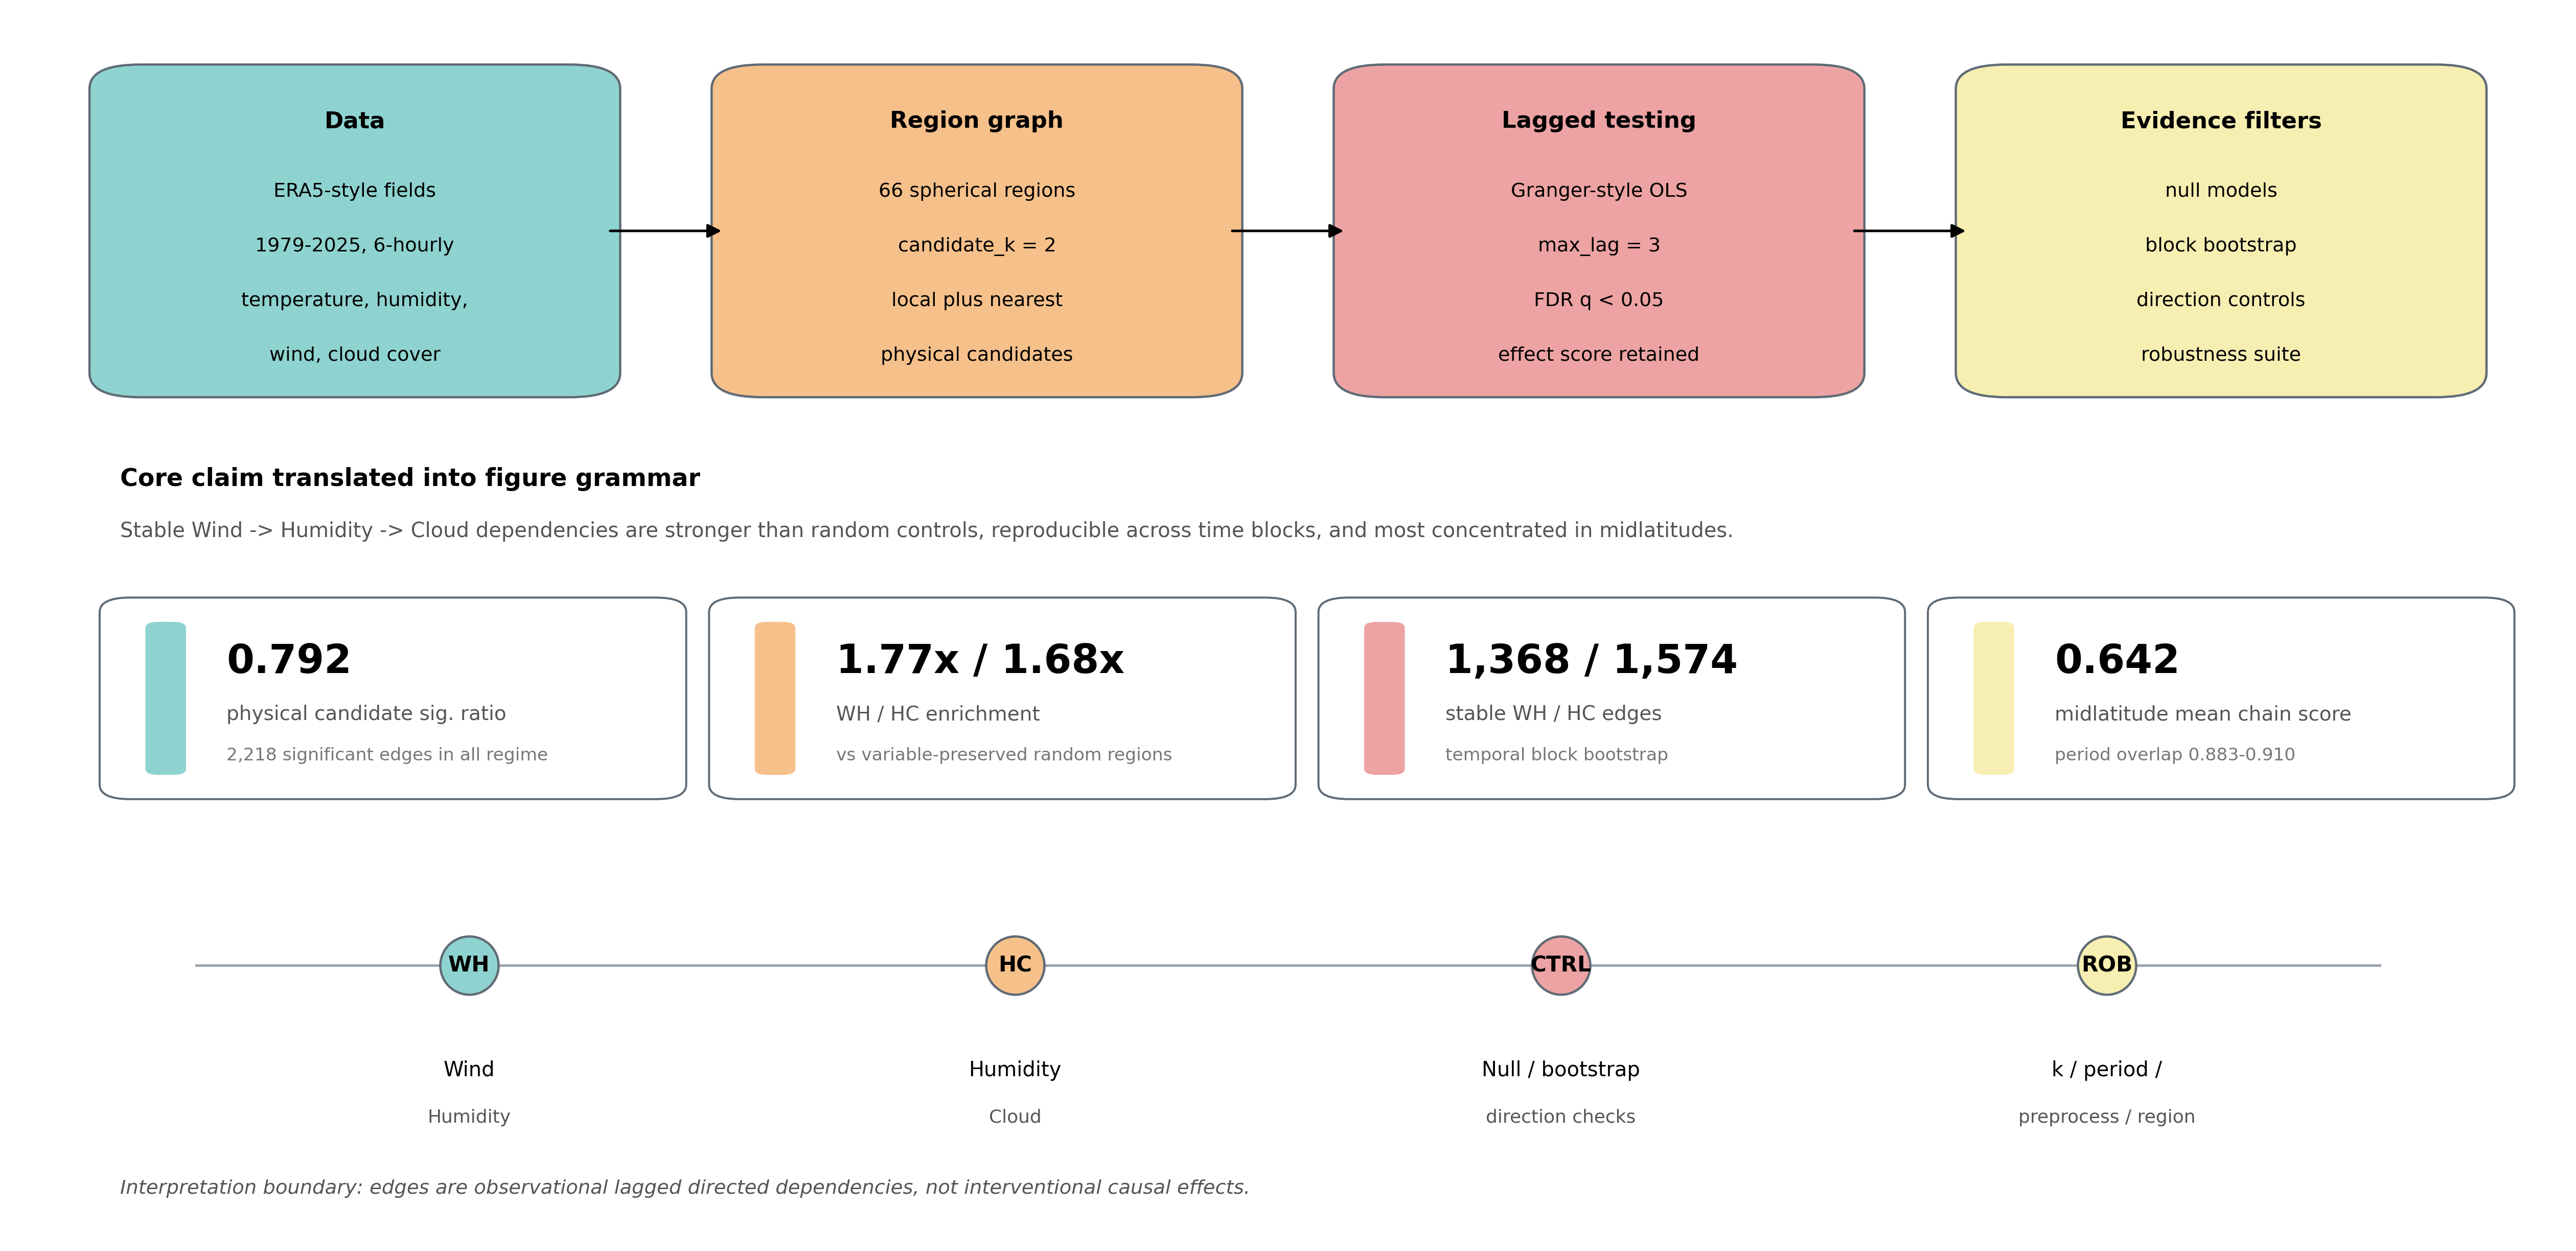
\includegraphics[width=0.98\textwidth]{figures/top_conference/fig01_evidence_stack.png}
}%DIFDELCMD < \caption{%
{%DIFAUXCMD
\DIFdelFL{Evidence stack of the main experiments: data scale, candidate graph, pathway statistics and robustness evidence for Wind $\rightarrow$ Humidity $\rightarrow$ Cloud Cover.}}
%DIFAUXCMD
%DIFDELCMD < \label{fig:1}
%DIFDELCMD < \end{figure}
%DIFDELCMD < 

%DIFDELCMD < \begin{table}[htbp]
%DIFDELCMD < \centering
%DIFDELCMD < %%%
%DIFDELCMD < \caption{%
{%DIFAUXCMD
\DIFdelFL{Main experimental results across regimes.}}
%DIFAUXCMD
%DIFDELCMD < \label{tab:2}
%DIFDELCMD < \scriptsize
%DIFDELCMD < \resizebox{\textwidth}{!}{%
%DIFDELCMD < \begin{tabular}{@{}llllllll@{}}
%DIFDELCMD < \toprule
%DIFDELCMD < Regime & Tested edges & Significant edges & Wind $\rightarrow$ Humidity fraction & Humidity $\rightarrow$ Cloud fraction & Cross-region fraction & Mean WH lag & Mean HC lag \\
%DIFDELCMD < \midrule
%DIFDELCMD < all & 2,574 & 2,218 & 0.227 & 0.220 & 0.599 & 2.006 & 1.977 \\
%DIFDELCMD < DJF & 2,574 & 2,017 & 0.243 & 0.213 & 0.590 & 1.992 & 1.979 \\
%DIFDELCMD < JJA & 2,574 & 2,023 & 0.218 & 0.218 & 0.589 & 1.975 & 1.989 \\
%DIFDELCMD < high\_humidity & 2,574 & 1,842 & 0.224 & 0.204 & 0.571 & 1.990 & 1.952 \\
%DIFDELCMD < normal\_humidity & 2,574 & 2,140 & 0.228 & 0.220 & 0.590 & 2.008 & 1.979 \\
%DIFDELCMD < high\_cloud & 2,574 & 1,843 & 0.231 & 0.213 & 0.571 & 1.988 & 1.969 \\
%DIFDELCMD < normal\_cloud & 2,574 & 2,191 & 0.227 & 0.220 & 0.595 & 2.000 & 1.969 \\
%DIFDELCMD < \bottomrule
%DIFDELCMD < \end{tabular}%
%DIFDELCMD < }
%DIFDELCMD < \end{table}
%DIFDELCMD < 

%DIFDELCMD < %%%
\subsection{\DIFdel{Spatial organization of the Wind--Humidity--Cloud Cover pathway}}
%DIFAUXCMD
\addtocounter{subsection}{-1}%DIFAUXCMD
%DIFDELCMD < 

%DIFDELCMD < %%%
\DIFdel{Pathway-level statistics showed that Wind $\rightarrow$ Humidity $\rightarrow$ Cloud Cover was not astructure assembled from a small number of local edges. In the all regime, 3, 746 WHC chains were identified, covering all 66 intermediate humidity regions. The mean total lag was 3.983 time steps, approximately }\DIFdelend \DIFaddbegin \DIFadd{discovery-period screening models, the median residual autocorrelation is close to zero at 6~h but 0.263 at }\DIFaddend 24\DIFdelbegin \DIFdel{hours. DJF contained 3, 215 chains with a mean chain score of 0.578,whereas JJA contained 2,998 chains with a mean chain score of 0.553}\DIFdelend \DIFaddbegin \DIFadd{~h, 0.215 at 72~h and 0.218 at 168~h (Figure~\ref{fig:calibration}a). With a month $\times$ UTC-hour climatology, these values fall to 0.099, 0.046 and 0.027, so most of the remaining dependence is the diurnal cycle that a monthly climatology leaves in the anomalies. Replacing the $F$-test with calendar-time HAC inference changes the screening counts only slightly: in the full-record, seven-regime screening, 13,995 rather than 14,308 of 18,018 tests pass within-family BH (Table~\ref{tab:regime})}\DIFaddend .

\begin{figure}[htbp]
\centering
\DIFdelbeginFL \DIFdelFL{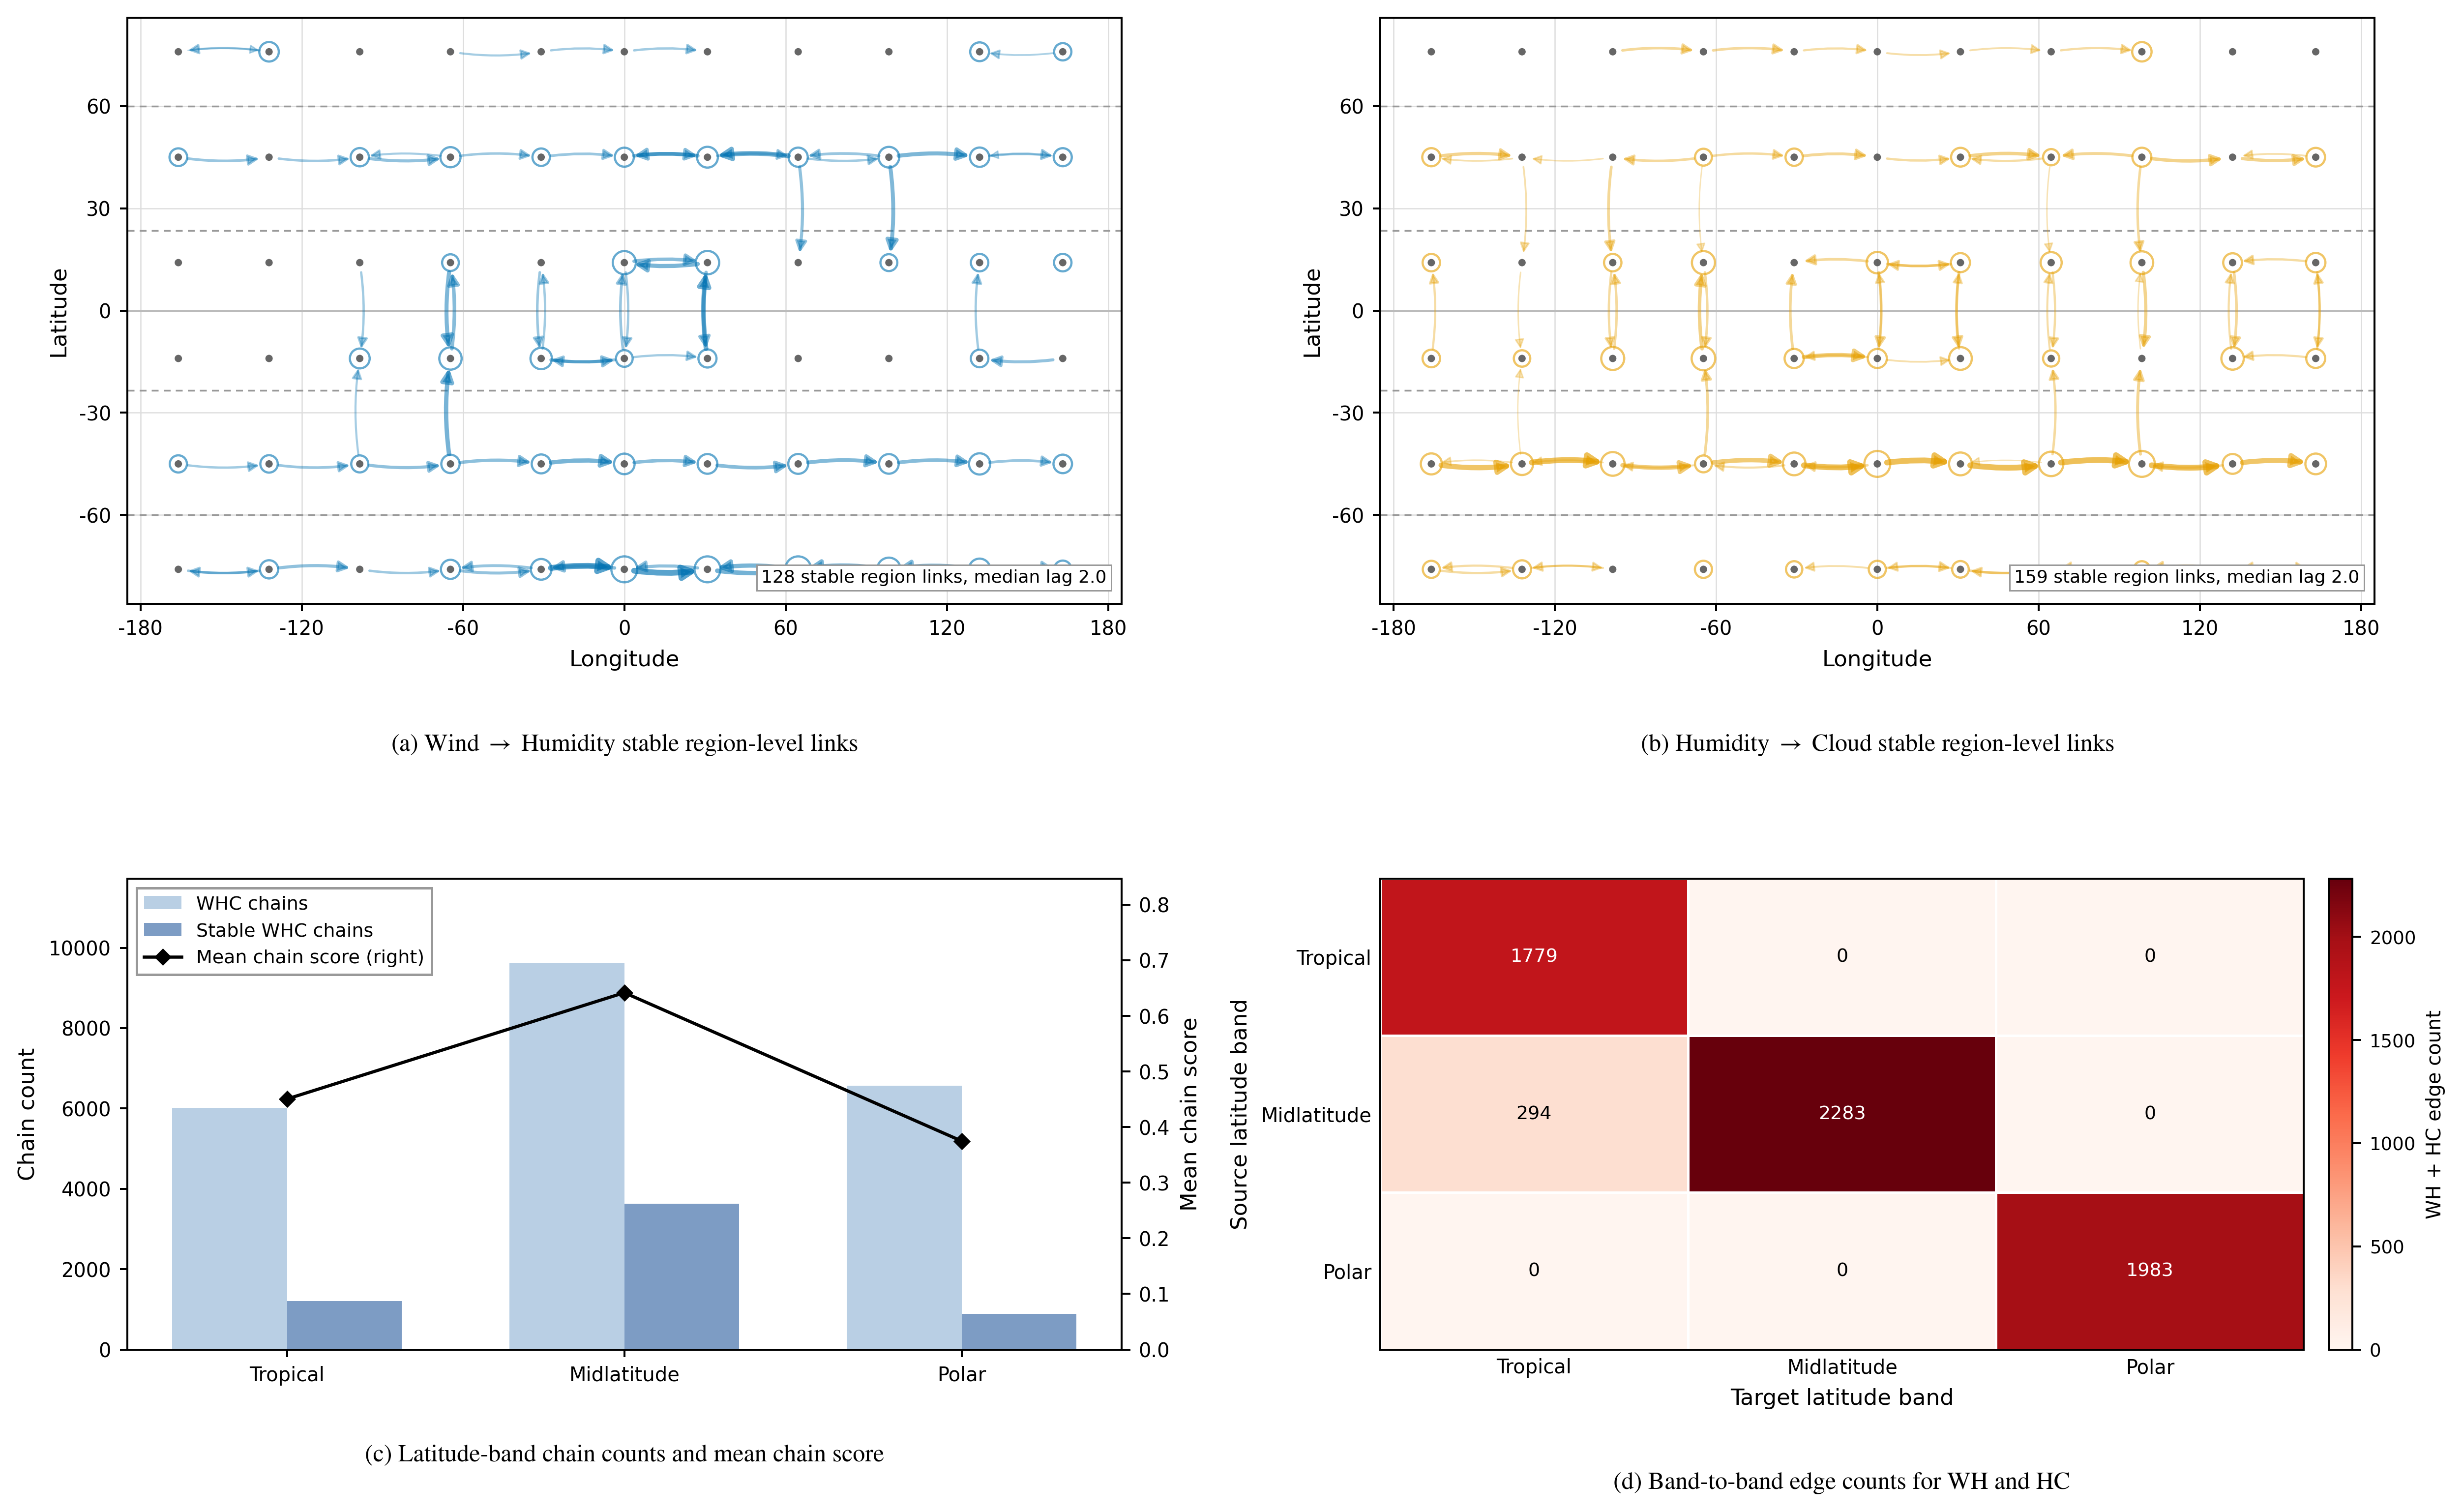
\includegraphics[width=0.98\textwidth]{figures/top_conference/fig02_spatial_pathway.png}
}\DIFdelendFL \DIFaddbeginFL \DIFaddFL{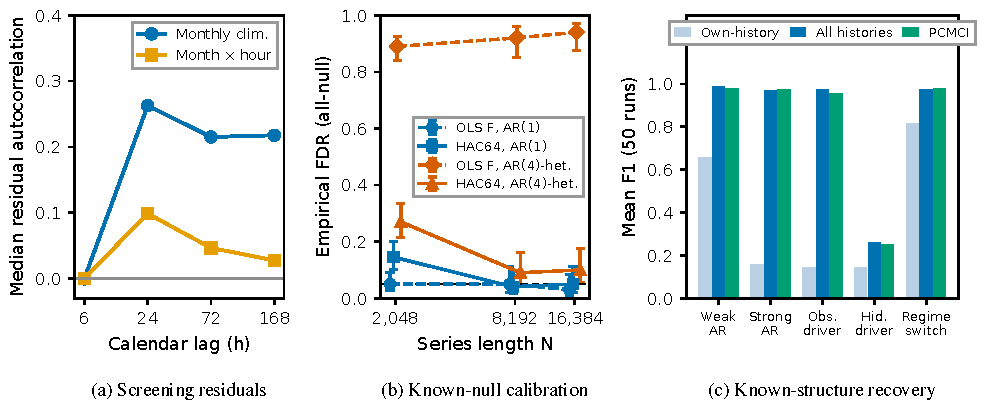
\includegraphics[width=\textwidth]{figures/fig02_calibration.pdf}
}\DIFaddendFL \caption{\DIFdelbeginFL \DIFdelFL{Spatial structure of the Wind $\rightarrow$ Humidity }\DIFdelendFL \DIFaddbeginFL \DIFaddFL{Residual dependence }\DIFaddendFL and \DIFdelbeginFL \DIFdelFL{Humidity $\rightarrow$ Cloud Cover edges}\DIFdelendFL \DIFaddbeginFL \DIFaddFL{calibration. Screening residuals are dominated by the diurnal cycle}\DIFaddendFL , \DIFdelbeginFL \DIFdelFL{separating local from cross-region dependencies}\DIFdelendFL \DIFaddbeginFL \DIFaddFL{OLS $F$-tests are badly miscalibrated under autoregressive heteroskedastic nulls whereas HAC inference approaches the nominal level as series lengthen, and own-history screening recovers structure poorly unless the system is weakly coupled}\DIFaddendFL .}
\DIFdelbeginFL %DIFDELCMD < \label{fig:2}
%DIFDELCMD < %%%
\DIFdelendFL \DIFaddbeginFL \label{fig:calibration}
\DIFaddendFL \end{figure}

\DIFdelbegin %DIFDELCMD < \begin{table}[htbp]
%DIFDELCMD < \centering
%DIFDELCMD < %%%
%DIFDELCMD < \caption{%
{%DIFAUXCMD
\DIFdelFL{Wind $\rightarrow$ Humidity $\rightarrow$ Cloud Cover chain statistics.}}
%DIFAUXCMD
%DIFDELCMD < \label{tab:3}
%DIFDELCMD < \scriptsize
%DIFDELCMD < \resizebox{\textwidth}{!}{%
%DIFDELCMD < \begin{tabular}{@{}lllll@{}}
%DIFDELCMD < \toprule
%DIFDELCMD < Regime & WHC chains & Intermediate humidity regions & Mean total lag & Mean chain score \\
%DIFDELCMD < \midrule
%DIFDELCMD < all & 3,746 & 66 & 3.983 & 0.468 \\
%DIFDELCMD < DJF & 3,215 & 66 & 3.976 & 0.578 \\
%DIFDELCMD < JJA & 2,998 & 66 & 3.963 & 0.553 \\
%DIFDELCMD < high\_humidity & 2,442 & 62 & 3.939 & 0.551 \\
%DIFDELCMD < normal\_humidity & 3,522 & 65 & 3.988 & 0.486 \\
%DIFDELCMD < high\_cloud & 2,612 & 65 & 3.962 & 0.499 \\
%DIFDELCMD < normal\_cloud & 3,667 & 66 & 3.972 & 0.468 \\
%DIFDELCMD < \bottomrule
%DIFDELCMD < \end{tabular}%
%DIFDELCMD < }
%DIFDELCMD < \end{table}
%DIFDELCMD < %%%
\DIFdelend \DIFaddbegin \DIFadd{The small change in counts does not imply that the $F$-tests were calibrated. In known-null simulations (Figure~\ref{fig:calibration}b), OLS $F$-tests attain the nominal false-discovery rate of 0.05 under autoregressive, homoskedastic noise, but under order-four heteroskedastic noise their empirical FDR is 0.890 at length 2,048 and 0.940 at 16,384, so a longer record does not help. HAC inference reduces the empirical FDR from 0.270 at length 2,048 to 0.100 (95\% interval 0.055--0.174) at 16,384, and from 0.475 to 0.070 when an external calendar mask removes part of the record. The discovery and held-out segments contain 58,437 and 5,884 responses, so HAC-based $q$-values are approximately but not exactly calibrated at our sample sizes. We therefore treat $q<0.05$ as a screening threshold and base our claims on held-out replication.

}\DIFaddend 

\DIFdelbegin \subsection{\DIFdel{Regime-aware analysis of state-dependent structure}}
%DIFAUXCMD
\addtocounter{subsection}{-1}%DIFAUXCMD
\DIFdelend \DIFaddbegin \DIFadd{Known-structure simulations expose a second, more serious problem (Figure~\ref{fig:calibration}c; Table~\ref{tab:benchmark}). Own-history screening recovers every true edge, but with strong autocorrelation its precision is 0.086 and its F1 is 0.158; with an observed common driver its F1 is 0.143, because indirect and common-driver dependencies are predictive given the target's own history alone. Regression on all observed histories restores F1 values of 0.970--0.986 and PCMCI 0.956--0.978. When the common driver is hidden, every method fails (F1 0.252--0.259). These results motivate confirmation under full conditioning and also bound what any method can achieve when relevant drivers are unobserved.

}\DIFaddend 

\DIFdelbegin \DIFdel{Regime comparison showed that the core pathway persisted under all major regimes, but pathway count and strength varied by state. The Wind $\rightarrow$ Humidity fraction was higher in DJF than in JJA,indicating stronger wind-to-moisture dependence under winter conditions. High\_humidity and high\_cloud regimes had fewer total significant edges than the corresponding normal regimes,but chain scores and mediation reductions were relatively higher,suggesting that humid or cloudy backgrounds may strengthen pathway intensity. }\DIFdelend \DIFaddbegin \subsection{\DIFadd{Screen, confirm, replicate}}
\label{subsec:three_res}

\DIFaddend 

\DIFdelbegin \DIFdel{The high-state samples were substantially smaller than their normal-state
counterparts, so we repeated the comparison after matched-size resampling. High humidity contained 13, 734 samples versus 41}\DIFdelend \DIFaddbegin \DIFadd{In 1979--2018, the own-history screen retains 2,187 of 2}\DIFaddend ,\DIFdelbegin \DIFdel{200 normal-humidity samples; high cloud contained 13, 734 samples versus 54, 934 normal-cloud samples. Across
20 matched repetitions, the mean Jaccard distances were 0.119 and 0.111,respectively, compared with original distances of 0.106 and 0.087. The
high-versus-matched-normal difference in total unique edge count was close to
zero for humidity states and 15.5 edges for cloud states. Thus, unequal sample
size explains part of the raw edge-count contrast but does not remove the state-dependent graph reorganization. }\DIFdelend \DIFaddbegin \DIFadd{574 edge--lag hypotheses, and full conditioning confirms 1,550 of them (Table~\ref{tab:threestage}; Figure~\ref{fig:threestage}a). Screening and confirmation disagree on sign for 649 of the 1,550 confirmed hypotheses, so own-history coefficient signs should not be interpreted. In the dense VAR, coefficients at different lags of the same edge alternate in sign for 95.2\% of the 568 confirmed edges with at least two confirmed lags, which indicates that much of the conditional dependence is carried by recent tendencies rather than levels. We therefore interpret magnitudes, replication and predictive gains rather than individual lag signs.

}\DIFaddend 

\DIFdelbegin %DIFDELCMD < \begin{figure}[htbp]
%DIFDELCMD < \centering
%DIFDELCMD < %%%
\DIFdelFL{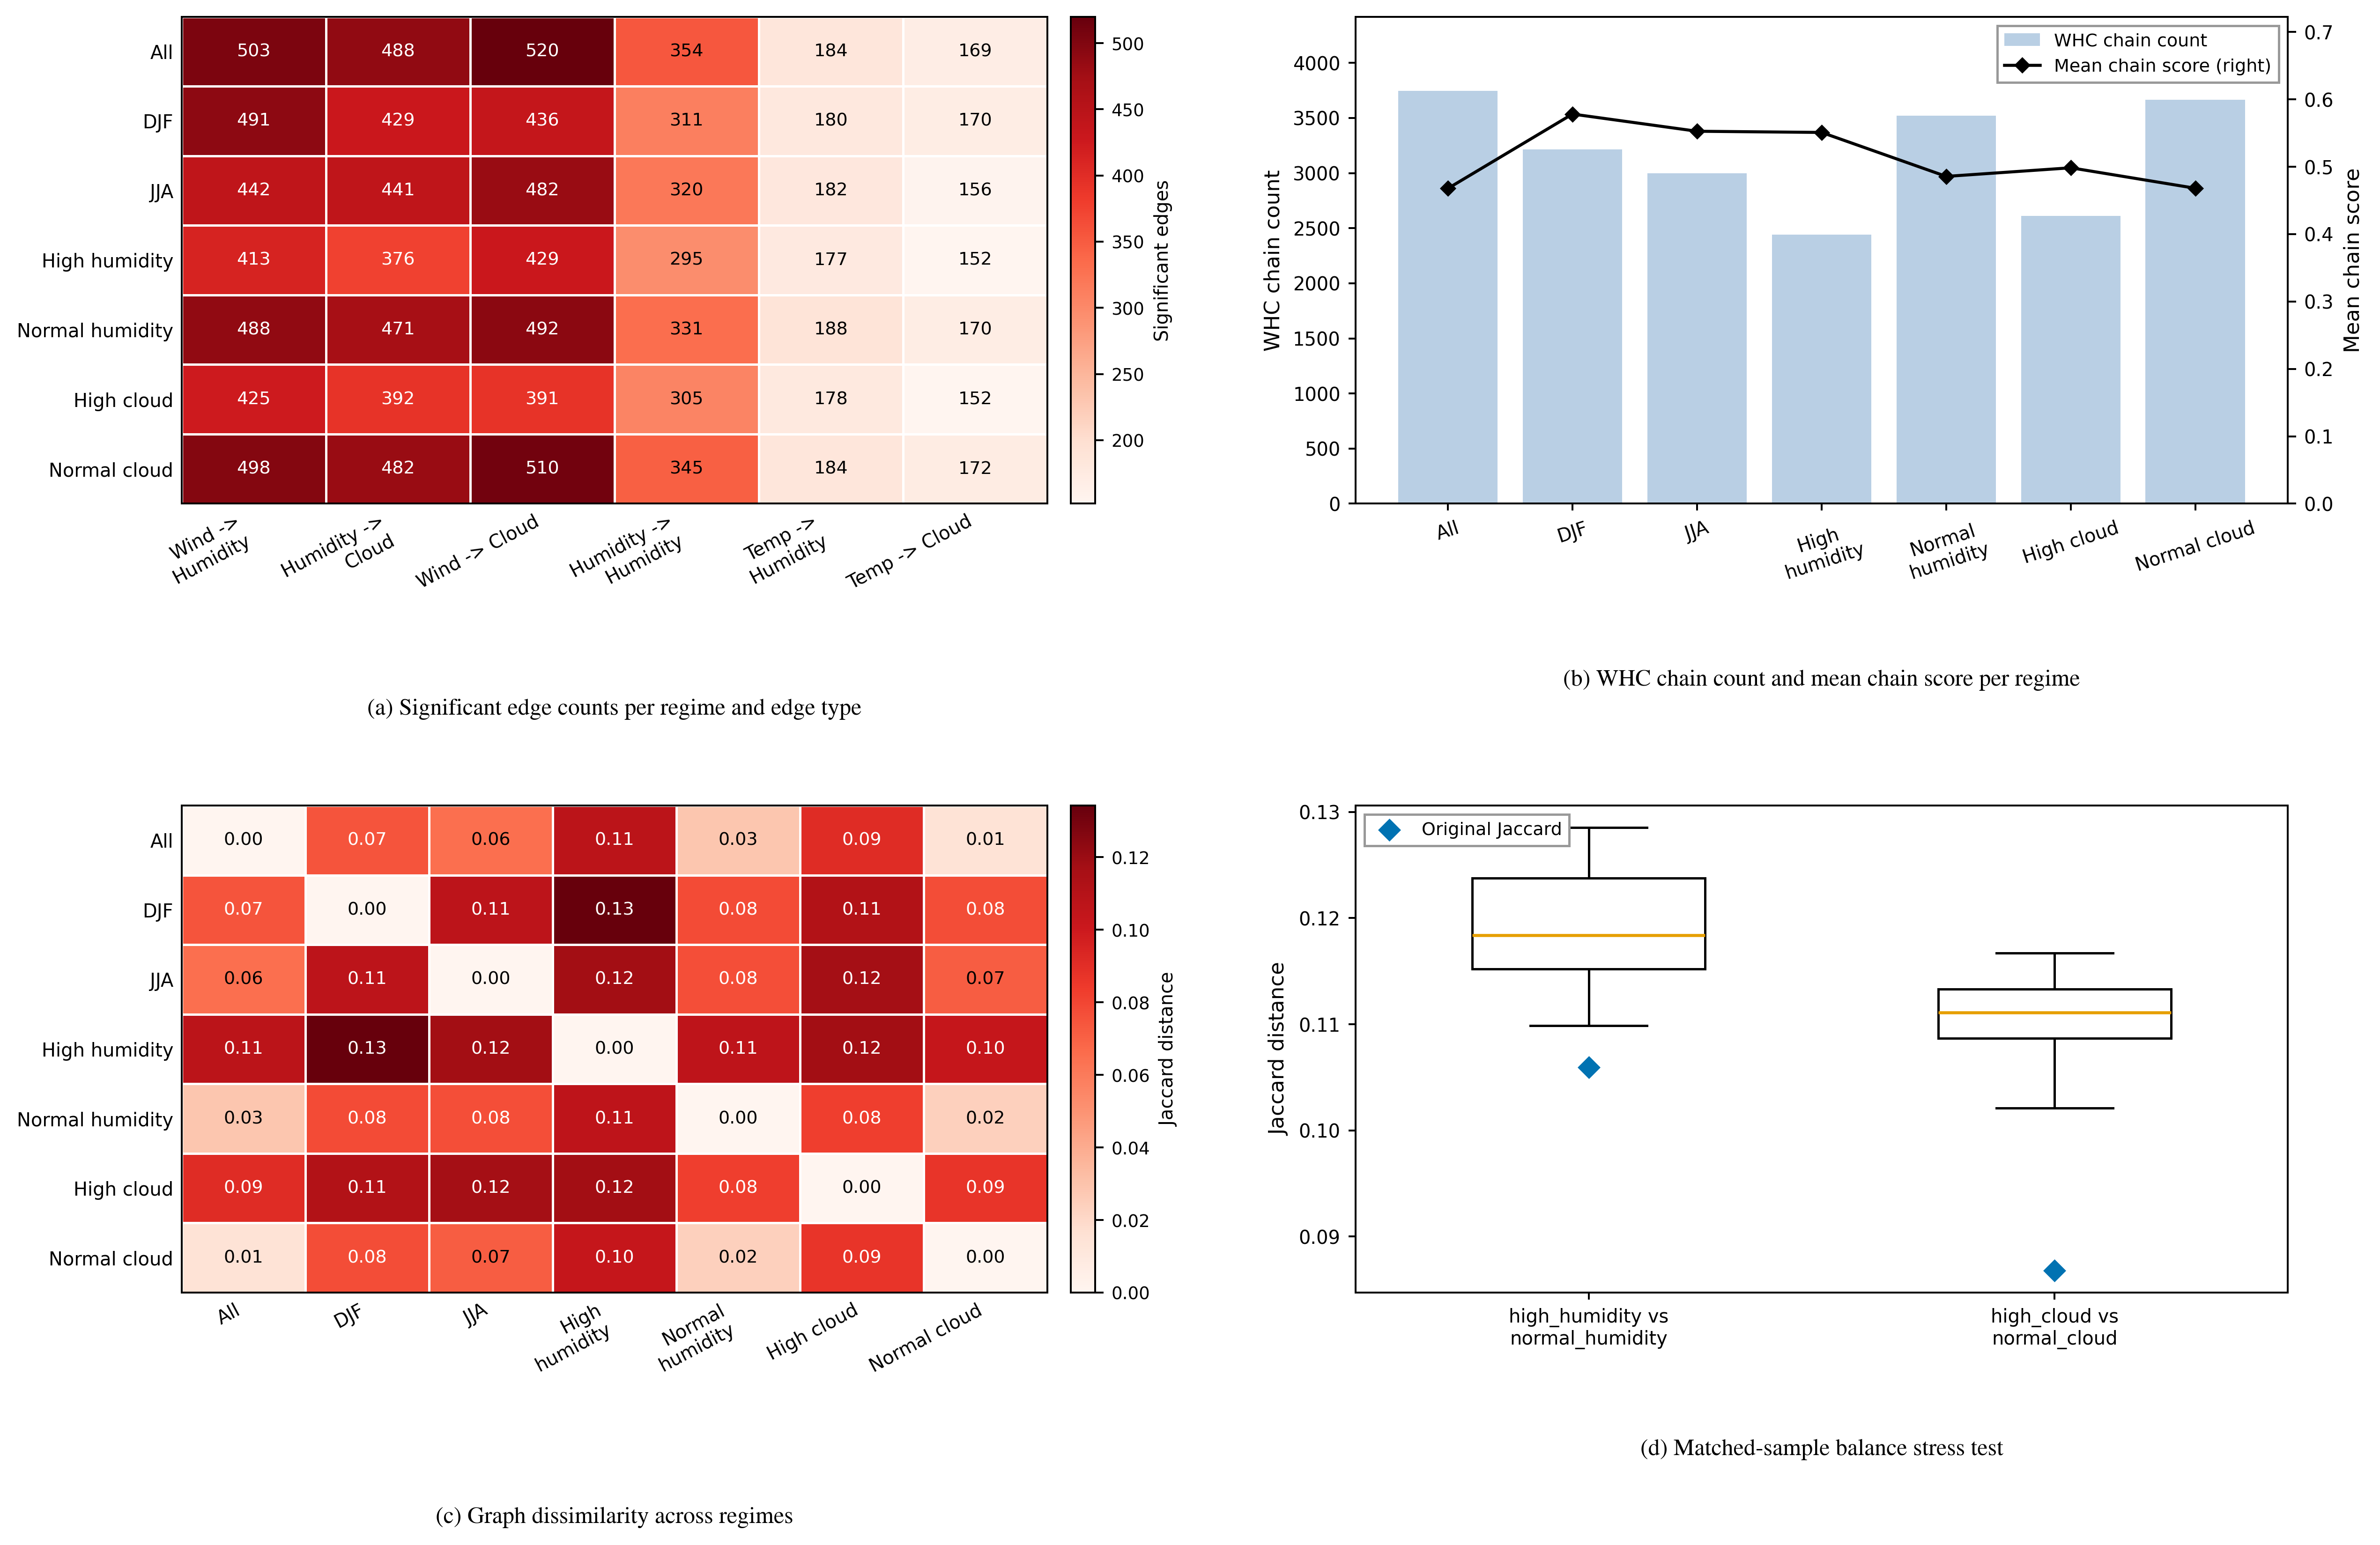
\includegraphics[width=0.98\textwidth]{figures/top_conference/fig03_regime_mechanism.png}
}%DIFDELCMD < \caption{%
{%DIFAUXCMD
\DIFdelFL{Regime dependence of the WHC pathway: chain counts and scores across seasonal, humidity-state and cloud-state regimes.}}
%DIFAUXCMD
%DIFDELCMD < \label{fig:3}
%DIFDELCMD < \end{figure}
%DIFDELCMD < 

%DIFDELCMD < %%%
\DIFdelend \begin{table}[htbp]
\centering
\caption{\DIFdelbeginFL \DIFdelFL{Regime graph differences measured }\DIFdelendFL \DIFaddbeginFL \DIFaddFL{Screen, confirm and replicate results }\DIFaddendFL by \DIFdelbeginFL \DIFdelFL{Jaccard distance}\DIFdelendFL \DIFaddbeginFL \DIFaddFL{edge type}\DIFaddendFL .}
\DIFdelbeginFL %DIFDELCMD < \label{tab:4}
%DIFDELCMD < %%%
\DIFdelendFL \DIFaddbeginFL \label{tab:threestage}
\DIFaddendFL \scriptsize
\DIFdelbeginFL %DIFDELCMD < \resizebox{\textwidth}{!}{%
%DIFDELCMD < \begin{tabular}{@{}llll@{}}
%DIFDELCMD < \toprule
%DIFDELCMD < Comparison & Jaccard distance & Union edges & Intersection edges \\
%DIFDELCMD < \midrule
%DIFDELCMD < DJF vs JJA & 0.107 & 851 & 760 \\
%DIFDELCMD < high\_humidity vs normal\_humidity & 0.106 & 840 & 751 \\
%DIFDELCMD < high\_cloud vs normal\_cloud & 0.087 & 841 & 768 \\
%DIFDELCMD < all vs DJF & 0.075 & 856 & 792 \\
%DIFDELCMD < all vs JJA & 0.065 & 851 & 796 \\
%DIFDELCMD < \bottomrule
%DIFDELCMD < \end{tabular}%
%DIFDELCMD < }
%DIFDELCMD < %%%
\DIFdelendFL \DIFaddbeginFL \setlength{\tabcolsep}{3.5pt}
\begin{tabular}{@{}lrrrrrrrrr@{}}
\toprule
& & \multicolumn{2}{c}{\DIFaddFL{1979--2018}} & \multicolumn{3}{c}{\DIFaddFL{2019-01-01 to 2023-01-10}} & \multicolumn{3}{c}{\DIFaddFL{2023-01-11 to 2025-12-31}} \\
\cmidrule(lr){3-4}\cmidrule(lr){5-7}\cmidrule(lr){8-10}
\DIFaddFL{Edge type }& \DIFaddFL{Tested }& \DIFaddFL{Screened }& \DIFaddFL{Confirmed }& \DIFaddFL{Replicated }& \DIFaddFL{Rate }& \shortstack[r]{\DIFaddFL{Control}\\\DIFaddFL{rate}} & \DIFaddFL{Replicated }& \DIFaddFL{Rate }& \shortstack[r]{\DIFaddFL{Control}\\\DIFaddFL{rate}} \\
\midrule
\DIFaddFL{$W\rightarrow H$ }& \DIFaddFL{594 }& \DIFaddFL{502 }& \DIFaddFL{325 }& \DIFaddFL{117 }& \DIFaddFL{0.360 }& \DIFaddFL{0.052 }& \DIFaddFL{101 }& \DIFaddFL{0.311 }& \DIFaddFL{0.059 }\\
\DIFaddFL{$H\rightarrow C$ }& \DIFaddFL{594 }& \DIFaddFL{480 }& \DIFaddFL{313 }& \DIFaddFL{133 }& \DIFaddFL{0.425 }& \DIFaddFL{0.100 }& \DIFaddFL{124 }& \DIFaddFL{0.396 }& \DIFaddFL{0.068 }\\
\DIFaddFL{$W\rightarrow C$ }& \DIFaddFL{594 }& \DIFaddFL{512 }& \DIFaddFL{311 }& \DIFaddFL{113 }& \DIFaddFL{0.363 }& \DIFaddFL{0.042 }& \DIFaddFL{92 }& \DIFaddFL{0.296 }& \DIFaddFL{0.032 }\\
\DIFaddFL{$H\rightarrow H$ }& \DIFaddFL{396 }& \DIFaddFL{342 }& \DIFaddFL{273 }& \DIFaddFL{153 }& \DIFaddFL{0.560 }& \DIFaddFL{0.138 }& \DIFaddFL{142 }& \DIFaddFL{0.520 }& \DIFaddFL{0.130 }\\
\DIFaddFL{$T\rightarrow H$ }& \DIFaddFL{198 }& \DIFaddFL{185 }& \DIFaddFL{171 }& \DIFaddFL{137 }& \DIFaddFL{0.801 }& \DIFaddFL{0.296 }& \DIFaddFL{121 }& \DIFaddFL{0.708 }& \DIFaddFL{0.259 }\\
\DIFaddFL{$T\rightarrow C$ }& \DIFaddFL{198 }& \DIFaddFL{166 }& \DIFaddFL{157 }& \DIFaddFL{107 }& \DIFaddFL{0.682 }& \DIFaddFL{0.390 }& \DIFaddFL{87 }& \DIFaddFL{0.554 }& \DIFaddFL{0.317 }\\
\midrule
\textit{\DIFaddFL{All}} & \DIFaddFL{2,574 }& \DIFaddFL{2,187 }& \DIFaddFL{1,550 }& \DIFaddFL{760 }& \DIFaddFL{0.490 }& \DIFaddFL{0.093 }& \DIFaddFL{667 }& \DIFaddFL{0.430 }& \DIFaddFL{0.078 }\\
\bottomrule
\end{tabular}
\DIFaddendFL \end{table}

\DIFdelbegin %DIFDELCMD < \begin{table}[htbp]
%DIFDELCMD < %%%
\DIFdelendFL \DIFaddbeginFL \begin{figure}[htbp]
\DIFaddendFL \centering
\DIFaddbeginFL \DIFaddFL{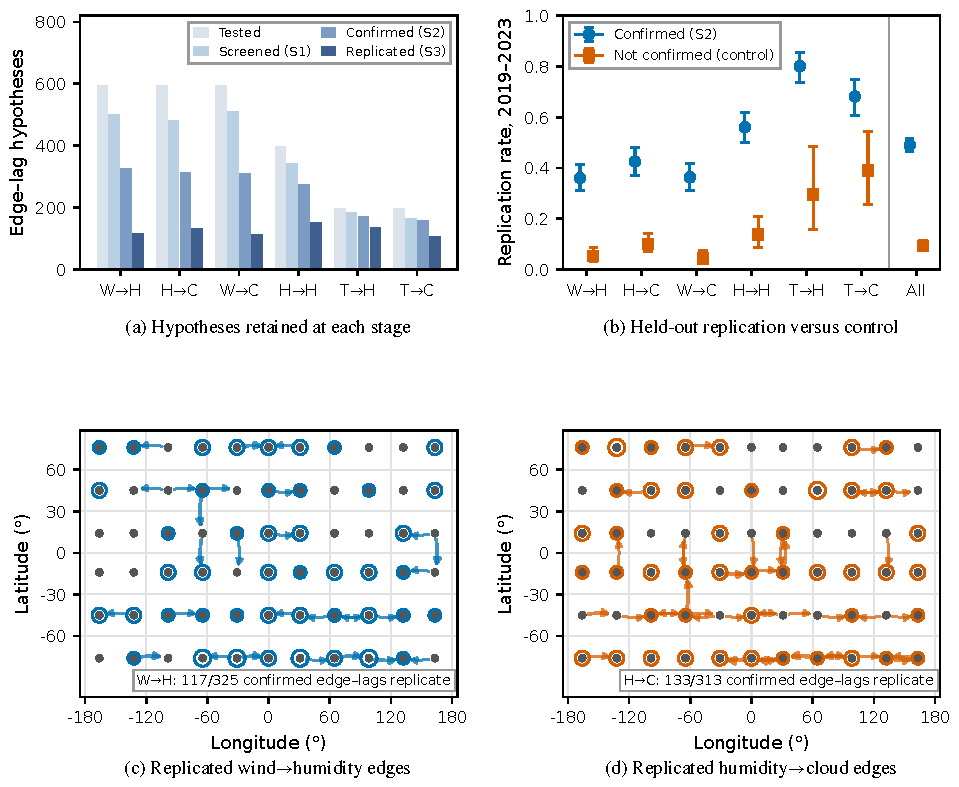
\includegraphics[width=\textwidth]{figures/fig03_three_stage.pdf}
}\DIFaddendFL \caption{\DIFdelbeginFL \DIFdelFL{Matched-sample sensitivity for high-state versus normal-state graphs}\DIFdelendFL \DIFaddbeginFL \DIFaddFL{Screen--confirm--replicate results}\DIFaddendFL . \DIFaddbeginFL \DIFaddFL{Confirmed hypotheses replicate far more often than unconfirmed controls, and replicated cross-region edges are predominantly zonal links between neighbouring regions.}\DIFaddendFL }
\DIFdelbeginFL %DIFDELCMD < \label{tab:sample_balance}
%DIFDELCMD < \scriptsize
%DIFDELCMD < \resizebox{\textwidth}{!}{%
%DIFDELCMD < \begin{tabular}{@{}lllllll@{}}
%DIFDELCMD < \toprule
%DIFDELCMD < Comparison & High samples & Normal samples & Original Jaccard & Matched Jaccard mean & Matched Jaccard SD & Mean edge-count difference \\
%DIFDELCMD < \midrule
%DIFDELCMD < high humidity vs normal humidity & 13,734 & 41,200 & 0.106 & 0.119 & 0.006 & -0.75 \\
%DIFDELCMD < high cloud vs normal cloud & 13,734 & 54,934 & 0.087 & 0.111 & 0.007 & 15.50 \\
%DIFDELCMD < \bottomrule
%DIFDELCMD < \end{tabular}%
%DIFDELCMD < }
%DIFDELCMD < \end{table}
%DIFDELCMD < %%%
\DIFdelend \DIFaddbegin \label{fig:threestage}
\end{figure}

\DIFaddend 

\DIFdelbegin \subsection{\DIFdel{Null-model and directionality control experiments}}
%DIFAUXCMD
\addtocounter{subsection}{-1}%DIFAUXCMD
%DIFDELCMD < 

%DIFDELCMD < %%%
\DIFdel{Null-model analysis showed that the core pathway could not be explained by random candidate edges or variable-type composition alone. The significant ratio of the physical candidate graph was 0.792,higher than fully random edges (0.513) }\DIFdelend \DIFaddbegin \DIFadd{In the primary held-out segment, 760 of the 1,550 confirmed hypotheses (0.490) replicate with the same sign, compared with 95 of the 1,024 unconfirmed hypotheses (0.093) under the identical rule (Figure~\ref{fig:threestage}b). Of the replicated hypotheses, 416 also improve frozen held-out prediction ($q<0.05$), }\DIFaddend and \DIFdelbegin \DIFdel{variable-preserved random edges (0.458) . Under the variable-preserved random control, Wind }\DIFdelend \DIFaddbegin \DIFadd{1,363 of the 1,550 confirmed hypotheses (0.879) keep their sign. Replication rates range from 0.360 for wind}\DIFaddend $\rightarrow$\DIFdelbegin \DIFdel{Humidity was enriched by 1.77-fold, Humidity }\DIFdelend \DIFaddbegin \DIFadd{humidity and 0.363 for wind}\DIFaddend $\rightarrow$\DIFdelbegin \DIFdel{Cloud Cover by 1.68-fold,and Wind }\DIFdelend \DIFaddbegin \DIFadd{cloud to 0.425 for humidity}\DIFaddend $\rightarrow$\DIFdelbegin \DIFdel{Cloud Cover by 1.93-fold. The distance-matched random graph still had a high significant ratio of 0.743, indicating that spatial-neighbour correlation is strong. Thus, the appropriate interpretation is not that the result is independent of spatial correlation,but that physically motivated pathways show additional enrichment within a strongly spatially correlated background.
}%DIFDELCMD < 

%DIFDELCMD < %%%
\DIFdel{Directionality controls showed that real temporal alignment was essential for the main pathway, but they did not establish a uniquely oriented causal graph.

The forward Wind }\DIFdelend \DIFaddbegin \DIFadd{cloud, 0.560 for humidity}\DIFaddend $\rightarrow$\DIFdelbegin \DIFdel{Humidity significant ratio was 0.781, higher than the reverse Humidity $\rightarrow$ Wind ratio of 0.639. After time shuffling, Wind $\rightarrow$ Humidity and Wind $\rightarrow$ Cloud Cover were reduced to zero significant edges }\DIFdelend \DIFaddbegin \DIFadd{humidity and 0.682--0.801 for the local temperature edges. The 760 replicated hypotheses correspond to 450 unique directed edges (of 726 confirmed unique edges); 300 hypotheses link different regions, and 249 of these connect regions in the same latitude row (Figure~\ref{fig:threestage}c,d). Replication is higher for midlatitude (0.531) and polar (0.521) than for tropical targets (0.411). In the second held-out segment, 2023-01-11 to 2025-12-31}\DIFaddend , \DIFdelbegin \DIFdel{and Humidity }\DIFdelend \DIFaddbegin \DIFadd{667 confirmed hypotheses (0.430) replicate against 80 of 1,024 controls (0.078), close to the primary segment despite its shorter length.

}

\DIFadd{Replicated dependencies are modest in size. The median absolute coefficient is 0.045 standard deviations for confirmed and 0.080 for replicated hypotheses, the median held-out partial $R^2$ of replicated hypotheses is 0.0029, and their median frozen relative reduction in mean squared error is 0.27\%. Summed over lags, 63\% of replicated humidity}\DIFaddend $\rightarrow$\DIFdelbegin \DIFdel{Cloud Cover was almost eliminated. Circular shifting reduced the significant ratios of the three main pathways to approximately 0.36--0.38. However, Cloud }\DIFdelend \DIFaddbegin \DIFadd{cloud edges and 90\% of temperature}\DIFaddend $\rightarrow$\DIFdelbegin \DIFdel{Humidity and future-to-past Humidity }\DIFdelend \DIFaddbegin \DIFadd{humidity edges are positive, whereas wind}\DIFaddend $\rightarrow$\DIFdelbegin \DIFdel{Cloud Cover remained strong. These controls therefore reject explanations based only on arbitrary time alignment, while also indicating bidirectional coupling,persistence or unresolved common forcing in the humidity--cloud subsystem}\DIFdelend \DIFaddbegin \DIFadd{cloud sums are evenly split. The three-stage results are insensitive to removing the diurnal cycle: with a month $\times$ UTC-hour climatology, 2,064 hypotheses are screened, 1,457 confirmed and 721 replicated, against 117 of 1,117 controls (Supplementary Table~S11). By contrast, PCMCI with partial-correlation tests and at most three conditioning variables, applied to all 2,574 hypotheses in 2019--2025, flags 85\% of the strongest screened hypotheses (top quartile of discovery effects), 82\% of the other screened hypotheses and 73\% of the unscreened hypotheses, so at this conditioning budget its agreement does not discriminate between strata}\DIFaddend .

\DIFdelbegin %DIFDELCMD < \begin{figure}[htbp]
%DIFDELCMD < \centering
%DIFDELCMD < %%%
\DIFdelFL{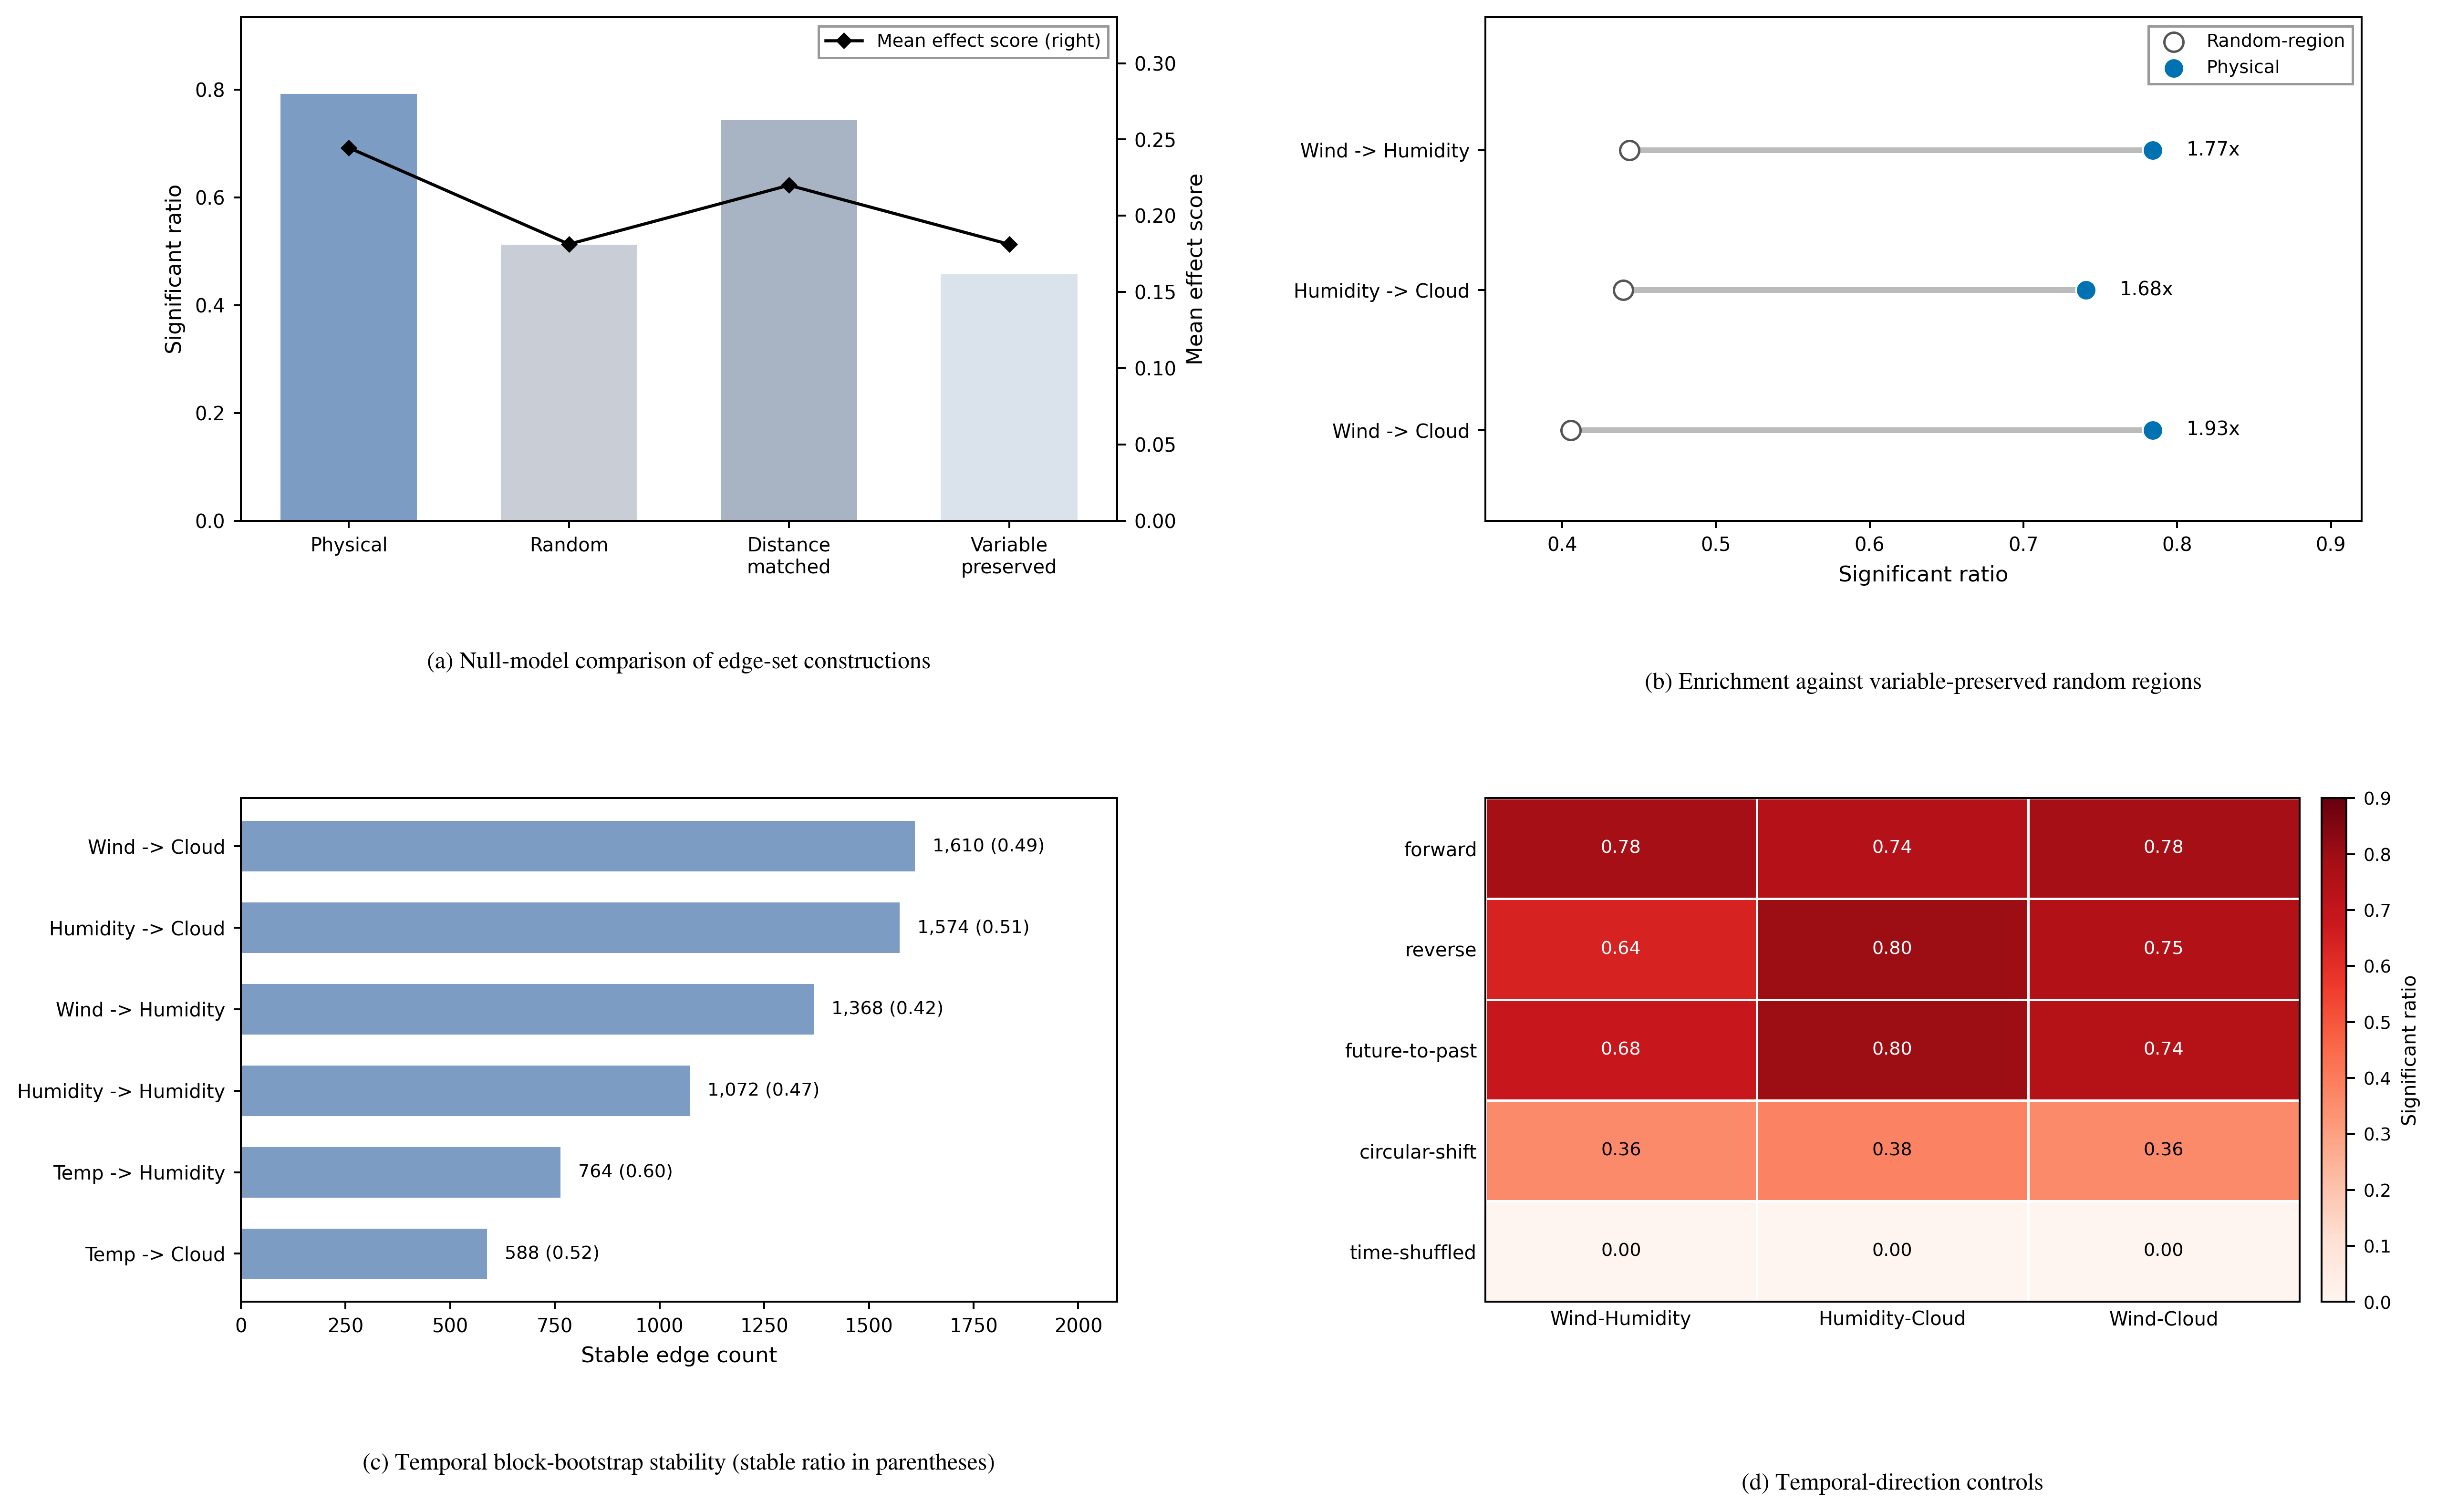
\includegraphics[width=0.98\textwidth]{figures/top_conference/fig04_controls.png}
}%DIFDELCMD < \caption{%
{%DIFAUXCMD
\DIFdelFL{Null-model and directionality controls: physical candidates versus random controls, and pathway behaviour under reversed, shuffled and circularly shifted time.}}
%DIFAUXCMD
%DIFDELCMD < \label{fig:4}
%DIFDELCMD < \end{figure}
%DIFDELCMD < %%%
\DIFdelend \DIFaddbegin \subsection{\DIFadd{Direction and spatial specificity}}
\label{subsec:dir_res}

\DIFaddend 

\DIFdelbegin %DIFDELCMD < \begin{table}[htbp]
%DIFDELCMD < \centering
%DIFDELCMD < %%%
%DIFDELCMD < \caption{%
{%DIFAUXCMD
\DIFdelFL{Null-model controls.}}
%DIFAUXCMD
%DIFDELCMD < \label{tab:5}
%DIFDELCMD < \scriptsize
%DIFDELCMD < \resizebox{\textwidth}{!}{%
%DIFDELCMD < \begin{tabular}{@{}llllll@{}}
%DIFDELCMD < \toprule
%DIFDELCMD < Edge set & Tested edges & Significant edges & Significant ratio & Mean absolute coefficient & Mean effect score \\
%DIFDELCMD < \midrule
%DIFDELCMD < physical\_candidates & 18,018 & 14,274 & 0.792 & 0.0228 & 0.2446 \\
%DIFDELCMD < random\_edges & 18,018 & 9,235 & 0.513 & 0.0186 & 0.1814 \\
%DIFDELCMD < distance\_matched\_random & 18,018 & 13,392 & 0.743 & 0.0208 & 0.2200 \\
%DIFDELCMD < variable\_preserved\_random & 18,018 & 8,244 & 0.458 & 0.0189 & 0.1813 \\
%DIFDELCMD < \bottomrule
%DIFDELCMD < \end{tabular}%
%DIFDELCMD < }
%DIFDELCMD < \end{table}
%DIFDELCMD < 

%DIFDELCMD < \begin{table}[htbp]
%DIFDELCMD < \centering
%DIFDELCMD < %%%
%DIFDELCMD < \caption{%
{%DIFAUXCMD
\DIFdelFL{Enrichment under variable-preserved random controls.}}
%DIFAUXCMD
%DIFDELCMD < \label{tab:6}
%DIFDELCMD < \scriptsize
%DIFDELCMD < \resizebox{\textwidth}{!}{%
%DIFDELCMD < \begin{tabular}{@{}llll@{}}
%DIFDELCMD < \toprule
%DIFDELCMD < Edge type & True significant ratio & Random-region significant ratio & Enrichment \\
%DIFDELCMD < \midrule
%DIFDELCMD < Wind $\rightarrow$ Humidity & 0.784 & 0.444 & 1.77 \\
%DIFDELCMD < Humidity $\rightarrow$ Cloud Cover & 0.741 & 0.440 & 1.68 \\
%DIFDELCMD < Wind $\rightarrow$ Cloud Cover & 0.784 & 0.406 & 1.93 \\
%DIFDELCMD < \bottomrule
%DIFDELCMD < \end{tabular}%
%DIFDELCMD < }
%DIFDELCMD < \end{table}
%DIFDELCMD < 

%DIFDELCMD < \begin{table}[htbp]
%DIFDELCMD < \centering
%DIFDELCMD < %%%
%DIFDELCMD < \caption{%
{%DIFAUXCMD
\DIFdelFL{Directionality and pseudo-time controls.}}
%DIFAUXCMD
%DIFDELCMD < \label{tab:7}
%DIFDELCMD < \scriptsize
%DIFDELCMD < \resizebox{\textwidth}{!}{%
%DIFDELCMD < \begin{tabular}{@{}llllll@{}}
%DIFDELCMD < \toprule
%DIFDELCMD < Test & Edge type & Tested edges & Significant edges & Significant ratio & Mean effect score \\
%DIFDELCMD < \midrule
%DIFDELCMD < forward & Wind $\rightarrow$ Humidity & 4,158 & 3,247 & 0.781 & 0.207 \\
%DIFDELCMD < reverse & Humidity $\rightarrow$ Wind & 4,158 & 2,655 & 0.639 & 0.123 \\
%DIFDELCMD < time\_shuffled & Wind $\rightarrow$ Humidity & 4,158 & 0 & 0.000 & 0.000 \\
%DIFDELCMD < circular\_shift & Wind $\rightarrow$ Humidity & 4,158 & 1,498 & 0.360 & 0.115 \\
%DIFDELCMD < forward & Humidity $\rightarrow$ Cloud Cover & 4,158 & 3,076 & 0.740 & 0.284 \\
%DIFDELCMD < reverse & Cloud $\rightarrow$ Humidity & 4,158 & 3,332 & 0.801 & 0.189 \\
%DIFDELCMD < time\_shuffled & Humidity $\rightarrow$ Cloud Cover & 4,158 & 1 & 0.000 & 0.063 \\
%DIFDELCMD < circular\_shift & Humidity $\rightarrow$ Cloud Cover & 4,158 & 1,585 & 0.381 & 0.120 \\
%DIFDELCMD < forward & Wind $\rightarrow$ Cloud Cover & 4,158 & 3,258 & 0.784 & 0.242 \\
%DIFDELCMD < time\_shuffled & Wind $\rightarrow$ Cloud Cover & 4,158 & 0 & 0.000 & 0.000 \\
%DIFDELCMD < \bottomrule
%DIFDELCMD < \end{tabular}%
%DIFDELCMD < }
%DIFDELCMD < \end{table}
%DIFDELCMD < 

%DIFDELCMD < %%%
\subsection{\DIFdel{Bootstrap stability, historical splits and robustness tests}}
%DIFAUXCMD
\addtocounter{subsection}{-1}%DIFAUXCMD
%DIFDELCMD < 

%DIFDELCMD < %%%
\DIFdel{Block bootstrap showed that the core edges were reproducible across long-term samples. Wind }\DIFdelend \DIFaddbegin \DIFadd{Under full conditioning, the direction of the humidity--cloud dependence becomes measurable, whereas that of the wind--humidity dependence does not (Table~\ref{tab:direction}; Figure~\ref{fig:direction}a). In 1979--2018, humidity}\DIFaddend $\rightarrow$\DIFdelbegin \DIFdel{Humidity had 3, 260 significant edges, of which 1, 368 met the stability criterion, with mean stability of 0.898. Humidity $\rightarrow$ Cloud Cover had 3, 079 significant edges, of which 1, 574 were stable, with mean stability of 0.887}\DIFdelend \DIFaddbegin \DIFadd{cloud has the larger absolute $t$-statistic in 55.2\% of 636 matched pairs (Wilcoxon $p=0.008$), and the asymmetry recurs in both held-out segments (52.2\%, $p=0.049$, in 2019--2023; 53.6\%, $p=0.023$, in 2023--2025), with diurnally adjusted anomalies (55.3\%, $p=0.005$) and with CERES cloud in 2017--2023 (56.3\%, $p=0.014$)}\DIFaddend . Wind$\rightarrow$\DIFdelbegin \DIFdel{Cloud Cover had 3, 260 significant edges, of which 1, 610 were stable, with mean stability of 0.890.
}%DIFDELCMD < 

%DIFDELCMD < %%%
\DIFdel{Historical-period analysis further showed that WH, HC, WC and WHC chains were retained across 1979-1989, 1990-1999, 2000-2009, 2010-2018 and 2019-2025. The overlap between each period graph and the full-period graph remained between 0.883 }\DIFdelend \DIFaddbegin \DIFadd{humidity is not stronger than humidity$\rightarrow$wind (48.4\%, $p=0.14$, in discovery; 48.3\%, $p=0.86$, in 2019--2023), }\DIFaddend and \DIFdelbegin \DIFdel{0.910}\DIFdelend \DIFaddbegin \DIFadd{in 2023--2025 the reverse is marginally stronger (45.8\%, $p=0.024$); wind--cloud pairs are balanced. This contrasts with own-history screening on the same symmetric support, where cloud$\rightarrow$humidity is significant more often than humidity$\rightarrow$cloud (547 versus 508 of 636) and wind$\rightarrow$humidity more often than its reverse (532 versus 475). Orientation inferred from own-history screening is therefore unreliable, and the wind--humidity direction of our pathway is a modelling choice rather than a data-supported finding}\DIFaddend .

\DIFdelbegin %DIFDELCMD < \begin{figure}[htbp]
%DIFDELCMD < \centering
%DIFDELCMD < %%%
\DIFdelFL{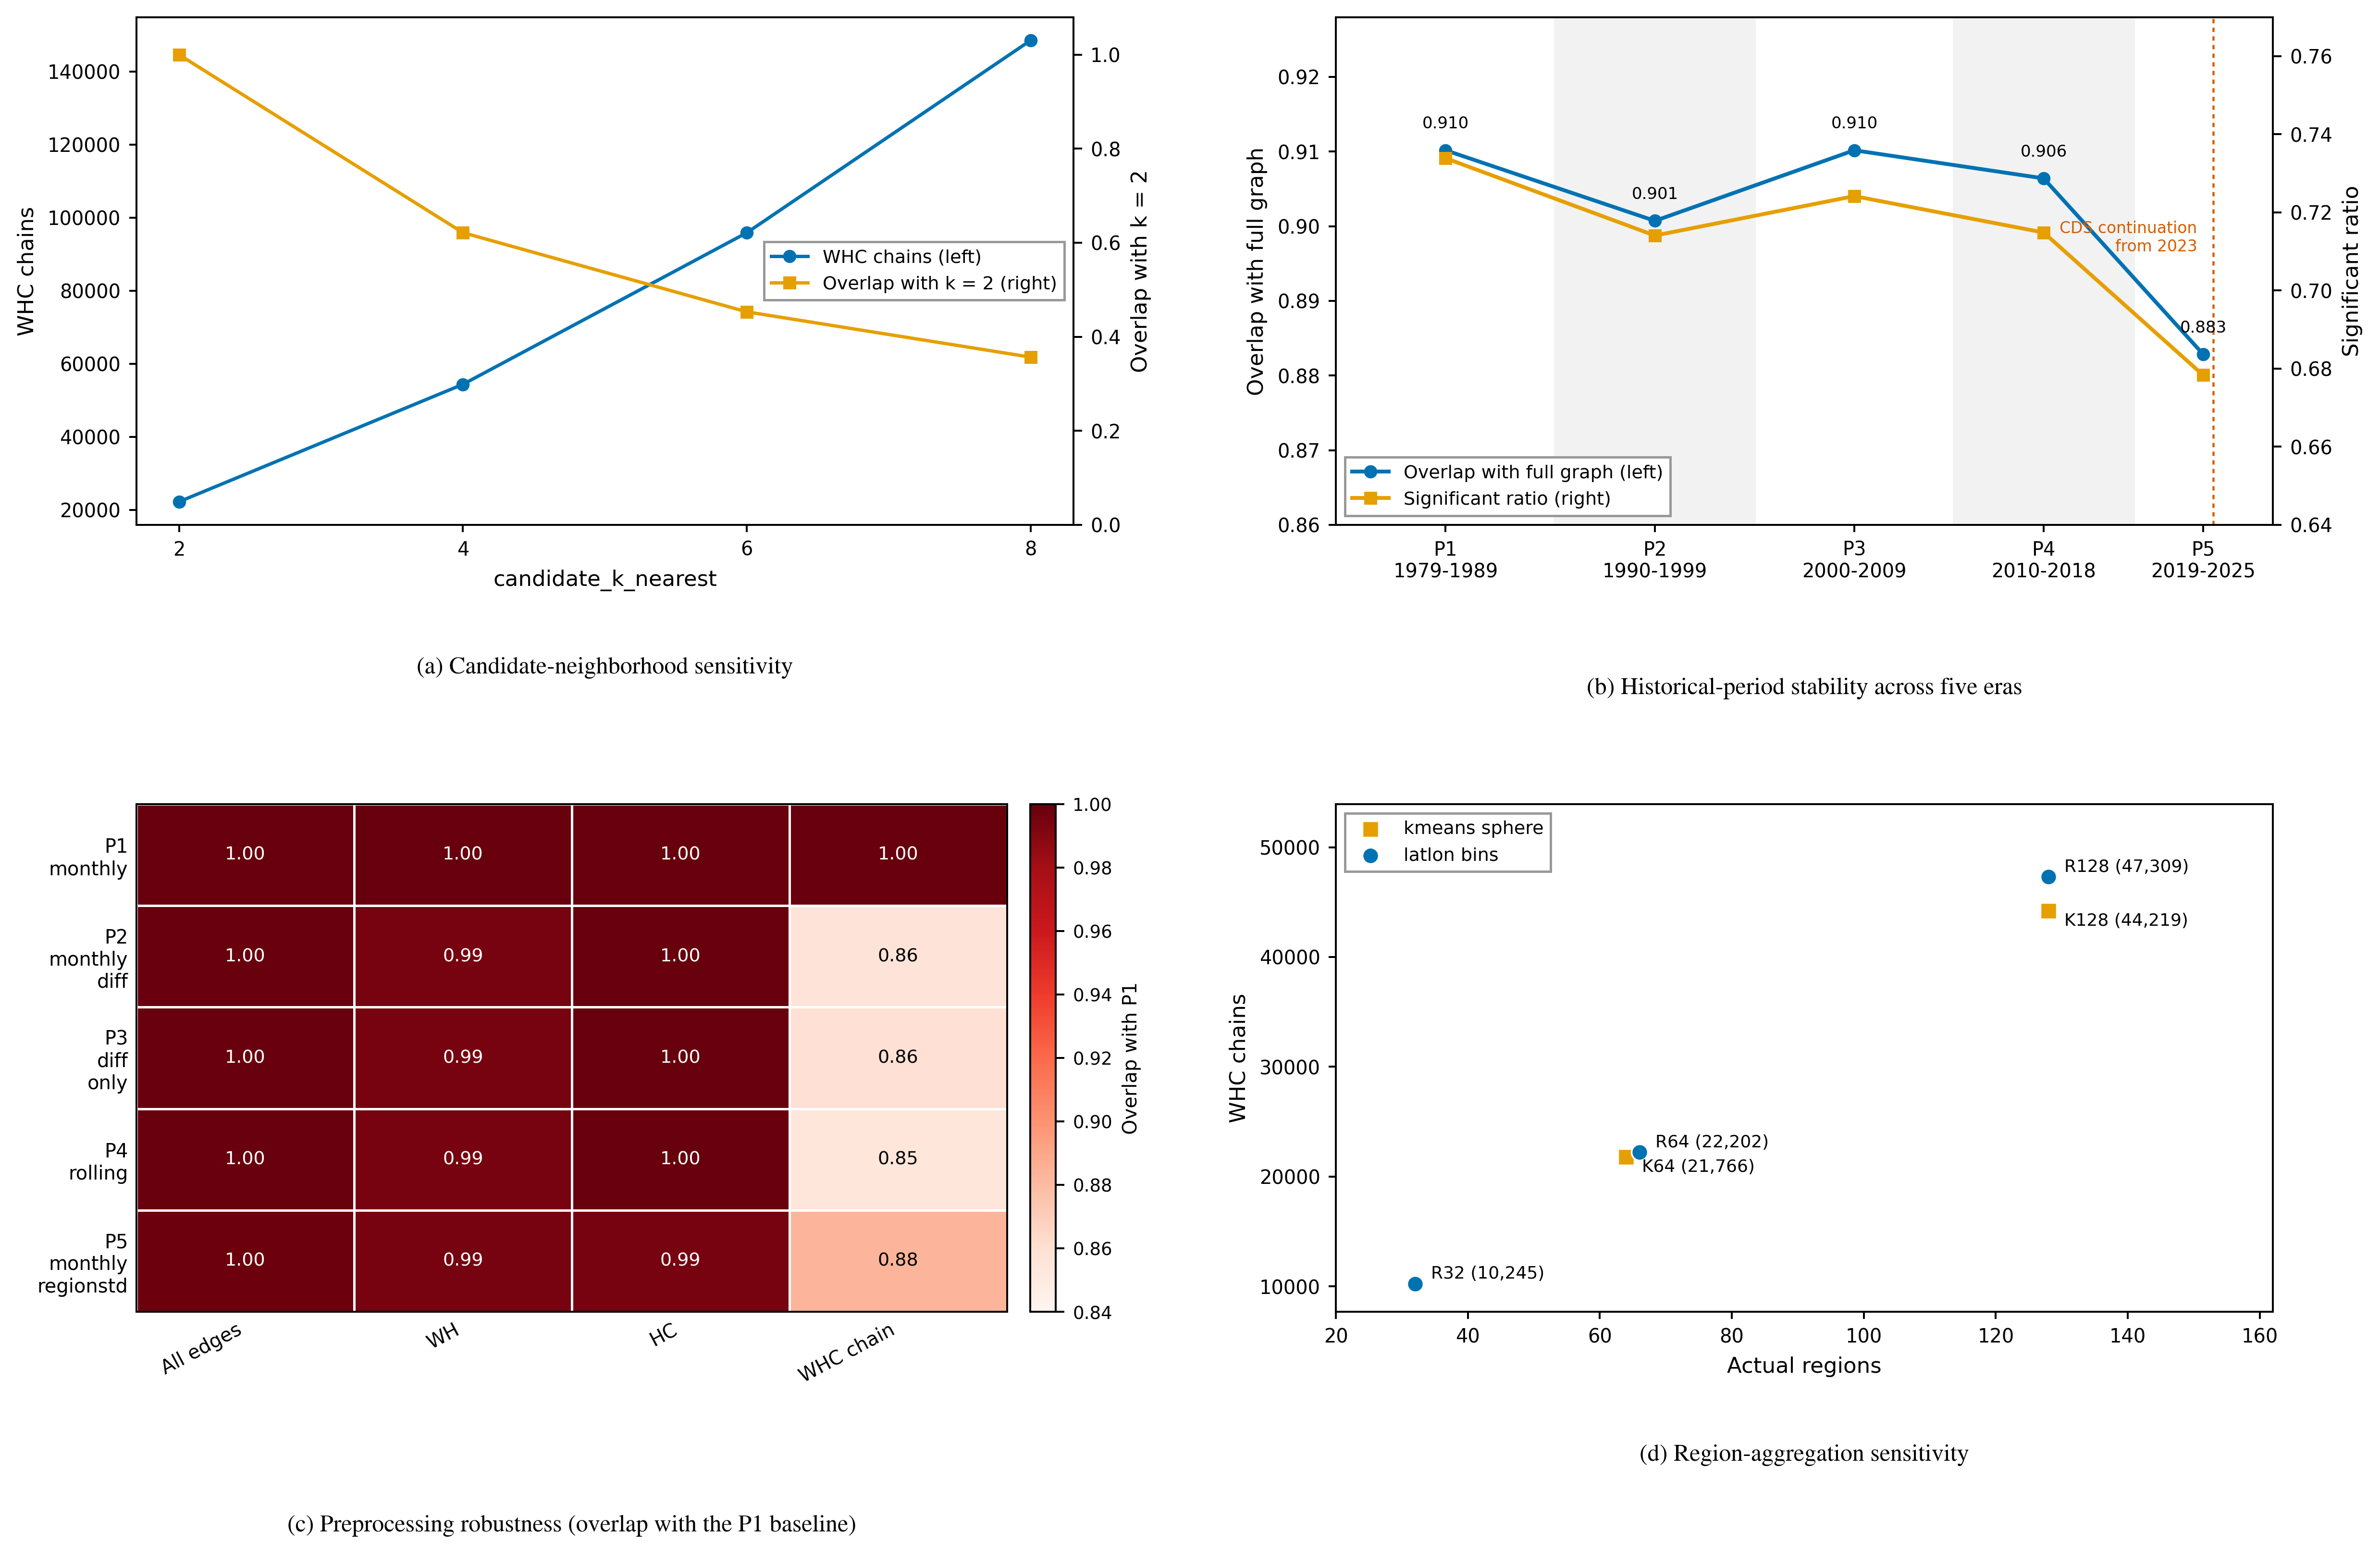
\includegraphics[width=0.98\textwidth]{figures/top_conference/fig05_robustness.png}
}%DIFDELCMD < \caption{%
{%DIFAUXCMD
\DIFdelFL{Robustness of the recovered structure under bootstrap, candidate-$k$, preprocessing and region-aggregation perturbations.}}
%DIFAUXCMD
%DIFDELCMD < \label{fig:5}
%DIFDELCMD < \end{figure}
%DIFDELCMD < 

%DIFDELCMD < %%%
\DIFdelend \begin{table}[htbp]
\centering
\caption{\DIFdelbeginFL \DIFdelFL{Bootstrap stability}\DIFdelendFL \DIFaddbeginFL \DIFaddFL{Direction tests on the symmetric candidate set under full conditioning}\DIFaddendFL .}
\DIFdelbeginFL %DIFDELCMD < \label{tab:8}
%DIFDELCMD < \scriptsize
%DIFDELCMD < \resizebox{\textwidth}{!}{%
%DIFDELCMD < \begin{tabular}{@{}lllll@{}}
%DIFDELCMD < \toprule
%DIFDELCMD < Edge type & Significant edges & Stable edges & Stable ratio & Mean stability \\
%DIFDELCMD < \midrule
%DIFDELCMD < Wind $\rightarrow$ Humidity & 3,260 & 1,368 & 0.420 & 0.898 \\
%DIFDELCMD < Humidity $\rightarrow$ Cloud Cover & 3,079 & 1,574 & 0.511 & 0.887 \\
%DIFDELCMD < Wind $\rightarrow$ Cloud Cover & 3,260 & 1,610 & 0.494 & 0.890 \\
%DIFDELCMD < Humidity $\rightarrow$ Humidity & 2,261 & 1,072 & 0.474 & 0.910 \\
%DIFDELCMD < Temperature $\rightarrow$ Humidity & 1,273 & 764 & 0.600 & 0.938 \\
%DIFDELCMD < Temperature $\rightarrow$ Cloud Cover & 1,141 & 588 & 0.515 & 0.895 \\
%DIFDELCMD < \bottomrule
%DIFDELCMD < \end{tabular}%
%DIFDELCMD < }
%DIFDELCMD < %%%
\DIFdelendFL \DIFaddbeginFL \label{tab:direction}
\footnotesize
\setlength{\tabcolsep}{3pt}
\begin{tabular}{@{}p{0.27\textwidth}lll@{}}
\toprule
\DIFaddFL{Measure }& \DIFaddFL{$H\rightarrow C$ vs $C\rightarrow H$ }& \DIFaddFL{$W\rightarrow H$ vs $H\rightarrow W$ }& \DIFaddFL{$W\rightarrow C$ vs $C\rightarrow W$ }\\
\midrule
\DIFaddFL{Significant, 1979--2018 }& \DIFaddFL{403 / 375 }& \DIFaddFL{381 / 402 }& \DIFaddFL{378 / 380 }\\
\DIFaddFL{Significant, 2019--2023 }& \DIFaddFL{118 / 115 }& \DIFaddFL{91 / 103 }& \DIFaddFL{89 / 88 }\\
\DIFaddFL{Significant, 2023--2025 }& \DIFaddFL{107 / 94 }& \DIFaddFL{78 / 77 }& \DIFaddFL{54 / 59 }\\
\DIFaddFL{Stronger forward, 1979--2018 }& \DIFaddFL{0.552 (0.008) }& \DIFaddFL{0.484 (0.142) }& \DIFaddFL{0.514 (0.379) }\\
\DIFaddFL{Stronger forward, 2019--2023 }& \DIFaddFL{0.522 (0.049) }& \DIFaddFL{0.483 (0.856) }& \DIFaddFL{0.508 (0.402) }\\
\DIFaddFL{Stronger forward, 2023--2025 }& \DIFaddFL{0.536 (0.023) }& \DIFaddFL{0.458 (0.024) }& \DIFaddFL{0.472 (0.103) }\\
\DIFaddFL{Stronger forward, diurnal, 2019--2023 }& \DIFaddFL{0.553 (0.005) }& \DIFaddFL{0.502 (0.481) }& \DIFaddFL{0.525 (0.466) }\\
\DIFaddFL{Stronger forward, CERES, 2017--2023 }& \DIFaddFL{0.563 (0.014) }& \DIFaddFL{-- }& \DIFaddFL{0.513 (0.288) }\\
\DIFaddFL{Stronger forward, CERES, 2023--2025 }& \DIFaddFL{0.494 (0.708) }& \DIFaddFL{-- }& \DIFaddFL{0.519 (0.334) }\\
\bottomrule
\end{tabular}
\DIFaddendFL \end{table}

\DIFdelbegin %DIFDELCMD < \begin{table}[htbp]
%DIFDELCMD < %%%
\DIFdelendFL \DIFaddbeginFL \begin{figure}[htbp]
\DIFaddendFL \centering
\DIFaddbeginFL \DIFaddFL{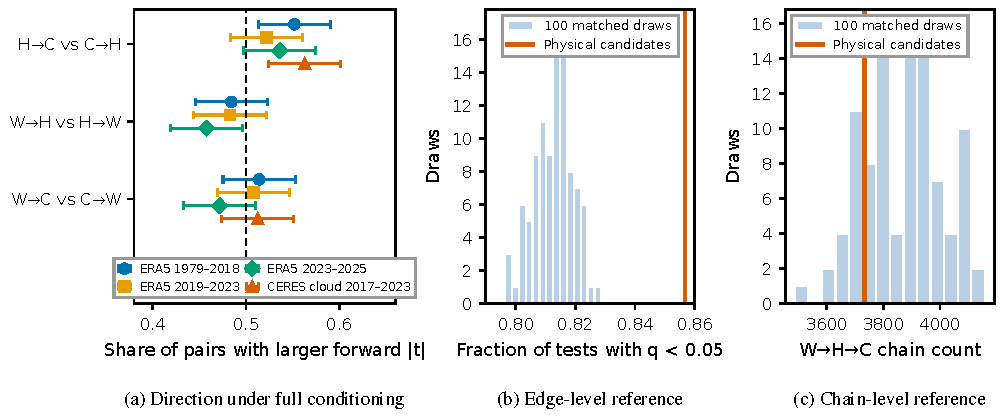
\includegraphics[width=\textwidth]{figures/fig04_direction_nulls.pdf}
}\DIFaddendFL \caption{\DIFdelbeginFL \DIFdelFL{Historical-period stability}\DIFdelendFL \DIFaddbeginFL \DIFaddFL{Direction and specificity}\DIFaddendFL . \DIFaddbeginFL \DIFaddFL{Only humidity$\rightarrow$cloud is consistently stronger than its reverse; physics-guided edges are significant more often than all 100 distance-matched random candidate sets, but their chain count lies inside the null distribution.}\DIFaddendFL }
\DIFdelbeginFL %DIFDELCMD < \label{tab:9}
%DIFDELCMD < \scriptsize
%DIFDELCMD < \resizebox{\textwidth}{!}{%
%DIFDELCMD < \begin{tabular}{@{}llllllll@{}}
%DIFDELCMD < \toprule
%DIFDELCMD < Period & Time range & Significant ratio & WH edges & HC edges & WC edges & WHC chains & Overlap with full graph \\
%DIFDELCMD < \midrule
%DIFDELCMD < P1 & 1979-1989 & 0.734 & 428 & 407 & 421 & 2,700 & 0.910 \\
%DIFDELCMD < P2 & 1990-1999 & 0.714 & 428 & 391 & 411 & 2,647 & 0.901 \\
%DIFDELCMD < P3 & 2000-2009 & 0.724 & 424 & 390 & 427 & 2,650 & 0.910 \\
%DIFDELCMD < P4 & 2010-2018 & 0.715 & 406 & 388 & 418 & 2,531 & 0.906 \\
%DIFDELCMD < P5 & 2019-2025 & 0.678 & 390 & 365 & 386 & 2,261 & 0.883 \\
%DIFDELCMD < \bottomrule
%DIFDELCMD < \end{tabular}%
%DIFDELCMD < }
%DIFDELCMD < \end{table}
%DIFDELCMD < %%%
\DIFdelend \DIFaddbegin \label{fig:direction}
\end{figure}

\DIFaddend 

\DIFdelbegin %DIFDELCMD < \begin{table}[htbp]
%DIFDELCMD < \centering
%DIFDELCMD < %%%
%DIFDELCMD < \caption{%
{%DIFAUXCMD
\DIFdelFL{Candidate-k robustness.}}
%DIFAUXCMD
%DIFDELCMD < \label{tab:10}
%DIFDELCMD < \scriptsize
%DIFDELCMD < \resizebox{\textwidth}{!}{%
%DIFDELCMD < \begin{tabular}{@{}lllllllll@{}}
%DIFDELCMD < \toprule
%DIFDELCMD < k & Candidate edges & Tested edges & Significant ratio & Unique significant edges & WH edges & HC edges & WHC chains & Recovered k=2 edges \\
%DIFDELCMD < \midrule
%DIFDELCMD < 2 & 858 & 18,018 & 0.792 & 857 & 3,260 & 3,079 & 22,202 & 857 \\
%DIFDELCMD < 4 & 1,386 & 29,106 & 0.746 & 1,379 & 4,956 & 4,926 & 54,351 & 857 \\
%DIFDELCMD < 6 & 1,914 & 40,194 & 0.697 & 1,892 & 6,400 & 6,655 & 95,871 & 857 \\
%DIFDELCMD < 8 & 2,442 & 51,282 & 0.672 & 2,403 & 7,804 & 8,376 & 148,573 & 857 \\
%DIFDELCMD < \bottomrule
%DIFDELCMD < \end{tabular}%
%DIFDELCMD < }
%DIFDELCMD < \end{table}
%DIFDELCMD < %%%
\DIFdelend \DIFaddbegin \DIFadd{The physics-guided candidates carry modest edge-level specificity beyond spatial background (Figure~\ref{fig:direction}b). In the full-record screen with HAC inference and global BH, 0.857 of the 2,574 hypotheses are significant, compared with a mean of 0.813 (2.5--97.5\% range 0.799--0.823) across 100 distance-matched random candidate sets, which the observed rate exceeds in every draw. The excess holds for wind$\rightarrow$humidity (0.857 versus 0.797), humidity$\rightarrow$cloud (0.808 versus 0.760) and wind$\rightarrow$cloud (0.874 versus 0.808). Chain abundance, by contrast, is not enriched: the physical graph contains 3,733 lag-resolved wind--humidity--cloud chains against a null mean of 3,871 (range 3,635--4,101; upper-tail probability 0.81), and on the symmetric support 4,249 against 4,288 (0.57). Chains that close a triad, in which wind also connects directly to the cloud target, are 1.60 times more frequent than in the null graphs (424 versus 264), which we attribute to spatial coherence among adjacent regions rather than to mediation.

}\DIFaddend 

\DIFaddbegin \subsection{\DIFadd{Regime and seasonal dependence}}
\label{subsec:regime_res}

\DIFadd{The descriptive full-record screen is nearly saturated in every regime (Table~\ref{tab:regime}). High-humidity and high-cloud regimes contain about one fifth of the responses and correspondingly fewer significant tests, and the shares of wind$\rightarrow$humidity, humidity$\rightarrow$cloud and cross-region edges vary by less than 0.04 across regimes. Because these regime graphs are selected separately, and the humidity and cloud masks condition on the response, their differences, including those in chain counts and Jaccard distances (Supplementary Table~S6), are not evidence of state dependence.

}

\DIFaddend \begin{table}[htbp]
\centering
\DIFdelbeginFL %DIFDELCMD < \caption{%
{%DIFAUXCMD
\DIFdelFL{Preprocessing robustness.}}
%DIFAUXCMD
%DIFDELCMD < \label{tab:11}
%DIFDELCMD < \scriptsize
%DIFDELCMD < \resizebox{\textwidth}{!}{%
%DIFDELCMD < \begin{tabular}{@{}lllllll@{}}
%DIFDELCMD < \toprule
%DIFDELCMD < Setting & Significant ratio & WH edges & HC edges & WC edges & WHC chains & WHC chain overlap \\
%DIFDELCMD < \midrule
%DIFDELCMD < P1\_monthly & 0.792 & 3,260 & 3,079 & 3,260 & 22,202 & 1.000 \\
%DIFDELCMD < P2\_monthly\_diff & 0.874 & 3,535 & 3,630 & 3,444 & 27,922 & 0.856 \\
%DIFDELCMD < P3\_diff\_only & 0.878 & 3,546 & 3,676 & 3,442 & 28,468 & 0.858 \\
%DIFDELCMD < P4\_rolling & 0.852 & 3,517 & 3,427 & 3,415 & 26,472 & 0.854 \\
%DIFDELCMD < P5\_monthly\_regionstd & 0.784 & 3,180 & 3,141 & 3,168 & 22,131 & 0.883 \\
%DIFDELCMD < \bottomrule
%DIFDELCMD < \end{tabular}%
%DIFDELCMD < }
%DIFDELCMD < %%%
\DIFdelendFL \DIFaddbeginFL \caption{\DIFaddFL{Descriptive full-record screening across regimes.}}
\label{tab:regime}
\footnotesize
\setlength{\tabcolsep}{4pt}
\begin{tabular}{@{}lrrrrrrr@{}}
\toprule
& & & \multicolumn{2}{c}{\DIFaddFL{Significant tests}} & \multicolumn{3}{c}{\DIFaddFL{Share of HAC-significant tests}} \\
\cmidrule(lr){4-5}\cmidrule(lr){6-8}
\DIFaddFL{Regime }& \DIFaddFL{Responses }& \DIFaddFL{Tests }& \DIFaddFL{OLS $F$ }& \DIFaddFL{HAC64 }& \DIFaddFL{$W\rightarrow H$ }& \DIFaddFL{$H\rightarrow C$ }& \DIFaddFL{Cross-region }\\
\midrule
\DIFaddFL{All }& \DIFaddFL{68,665 }& \DIFaddFL{2,574 }& \DIFaddFL{2,233 }& \DIFaddFL{2,206 }& \DIFaddFL{0.231 }& \DIFaddFL{0.218 }& \DIFaddFL{0.599 }\\
\DIFaddFL{DJF }& \DIFaddFL{16,965 }& \DIFaddFL{2,574 }& \DIFaddFL{2,010 }& \DIFaddFL{1,962 }& \DIFaddFL{0.243 }& \DIFaddFL{0.214 }& \DIFaddFL{0.584 }\\
\DIFaddFL{JJA }& \DIFaddFL{17,296 }& \DIFaddFL{2,574 }& \DIFaddFL{2,026 }& \DIFaddFL{2,001 }& \DIFaddFL{0.218 }& \DIFaddFL{0.220 }& \DIFaddFL{0.589 }\\
\DIFaddFL{High humidity }& \DIFaddFL{13,731 }& \DIFaddFL{2,574 }& \DIFaddFL{1,863 }& \DIFaddFL{1,790 }& \DIFaddFL{0.230 }& \DIFaddFL{0.211 }& \DIFaddFL{0.573 }\\
\DIFaddFL{Normal humidity }& \DIFaddFL{41,200 }& \DIFaddFL{2,574 }& \DIFaddFL{2,144 }& \DIFaddFL{2,104 }& \DIFaddFL{0.232 }& \DIFaddFL{0.220 }& \DIFaddFL{0.588 }\\
\DIFaddFL{High cloud }& \DIFaddFL{13,734 }& \DIFaddFL{2,574 }& \DIFaddFL{1,849 }& \DIFaddFL{1,776 }& \DIFaddFL{0.239 }& \DIFaddFL{0.206 }& \DIFaddFL{0.565 }\\
\DIFaddFL{Normal cloud }& \DIFaddFL{54,931 }& \DIFaddFL{2,574 }& \DIFaddFL{2,183 }& \DIFaddFL{2,156 }& \DIFaddFL{0.231 }& \DIFaddFL{0.218 }& \DIFaddFL{0.596 }\\
\midrule
\DIFaddFL{Total }& \DIFaddFL{-- }& \DIFaddFL{18,018 }& \DIFaddFL{14,308 }& \DIFaddFL{13,995 }& \DIFaddFL{-- }& \DIFaddFL{-- }& \DIFaddFL{-- }\\
\bottomrule
\end{tabular}
\DIFaddendFL \end{table}

\DIFdelbegin %DIFDELCMD < \begin{table}[htbp]
%DIFDELCMD < %%%
\DIFdelendFL \DIFaddbeginFL \DIFaddFL{Direct interaction tests separate state dependence from selection (Figure~\ref{fig:regimes}c). Source-by-cloud-state interactions pass BH in 173 of 2,574 tests in 1979--2018 when the state is concurrent and in 124 when it is defined 24~h earlier, but in only 4 and 1 of the 2,574 held-out tests. Humidity-state interactions fall from 117 and 107 discovery tests to 36 and 37 held-out tests. External states defined from the antecedent Ni\~no-3.4 anomaly give small slope contrasts whose signs change in 30 of 108 high-minus-middle and 24 of 108 low-minus-middle comparisons once the six physical controls are added (Supplementary Table~S7). We therefore find no replicable modulation of the dependencies by cloud or ENSO state at this design, and only weak modulation by the humidity state.

}

\begin{figure}[htbp]
\DIFaddendFL \centering
\DIFdelbeginFL %DIFDELCMD < \caption{%
{%DIFAUXCMD
\DIFdelFL{Region-aggregation robustness.}}
%DIFAUXCMD
%DIFDELCMD < \label{tab:12}
%DIFDELCMD < \scriptsize
%DIFDELCMD < \resizebox{\textwidth}{!}{%
%DIFDELCMD < \begin{tabular}{@{}lllllllll@{}}
%DIFDELCMD < \toprule
%DIFDELCMD < Setting & Method & Actual regions & Significant ratio & WH edges & HC edges & WC edges & WHC chains & Midlatitude strongest \\
%DIFDELCMD < \midrule
%DIFDELCMD < R32 & latlon\_bins & 32 & 0.785 & 1,491 & 1,498 & 1,573 & 10,245 & no \\
%DIFDELCMD < R64 & latlon\_bins & 66 & 0.792 & 3,260 & 3,079 & 3,260 & 22,202 & yes \\
%DIFDELCMD < R128 & latlon\_bins & 128 & 0.822 & 6,460 & 6,488 & 6,358 & 47,309 & yes \\
%DIFDELCMD < K64 & kmeans\_sphere & 64 & 0.791 & 3,035 & 3,161 & 3,159 & 21,766 & yes \\
%DIFDELCMD < K128 & kmeans\_sphere & 128 & 0.804 & 6,075 & 6,474 & 6,359 & 44,219 & yes \\
%DIFDELCMD < \bottomrule
%DIFDELCMD < \end{tabular}%
%DIFDELCMD < }
%DIFDELCMD < \end{table}
%DIFDELCMD < %%%
\DIFdelend \DIFaddbegin \DIFadd{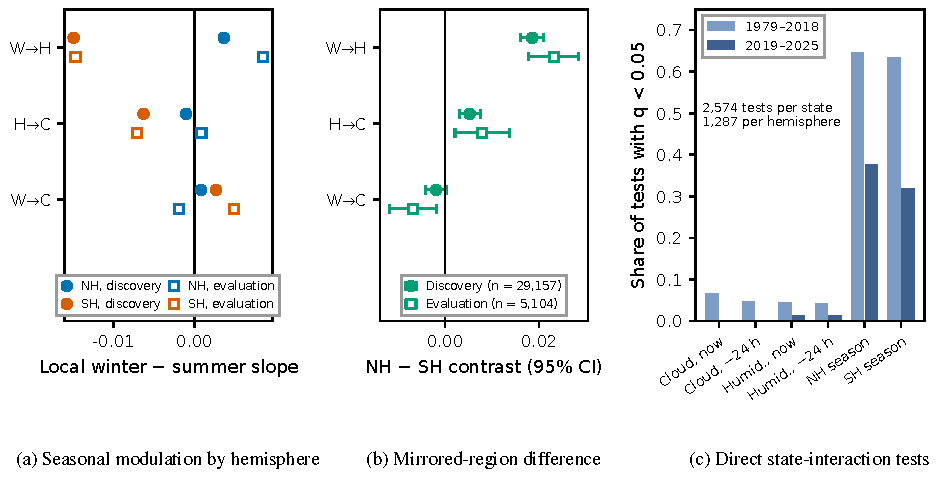
\includegraphics[width=\textwidth]{figures/fig05_regimes.pdf}
}\caption{\DIFadd{Seasonal and state dependence. Seasonal modulation of wind$\rightarrow$humidity has opposite signs in the two hemispheres, and cloud-state interactions found in 1979--2018 do not replicate in 2019--2025.}}
\label{fig:regimes}
\end{figure}

\DIFaddend 

\DIFdelbegin \subsection{\DIFdel{Latitude-band, long-lag and humidity-mediation analyses}}
%DIFAUXCMD
\addtocounter{subsection}{-1}%DIFAUXCMD
\DIFdelend \DIFaddbegin \DIFadd{Seasonal modulation, in contrast, is pervasive and replicates: local winter-minus-summer slope differences pass BH in 830 and 816 of 1,287 discovery tests in the NH and SH and in 485 and 411 held-out tests. Its sign, however, differs between hemispheres (Figure~\ref{fig:regimes}a). For wind$\rightarrow$humidity, the mean signed winter-minus-summer slope is $+0.0036$ in the NH and $-0.0149$ in the SH in 1979--2018 ($+0.0084$ and $-0.0147$ in 2019--2025), and the mirrored-region contrast $\Delta_{\mathrm{NH}}-\Delta_{\mathrm{SH}}$ is $0.0185$ (95\% interval $0.0160$--$0.0210$) in discovery and $0.0231$ ($0.0178$--$0.0284$) held out (Figure~\ref{fig:regimes}b). Humidity$\rightarrow$cloud shows a smaller contrast ($0.0053$ and $0.0079$), and wind$\rightarrow$cloud none in discovery ($-0.0019$, $-0.0040$ to $0.0003$) and a small negative one held out ($-0.0068$, $-0.0118$ to $-0.0017$). A globally pooled DJF regime therefore mixes NH winter with SH summer, and the dependencies do not strengthen uniformly in winter.

}\DIFaddend 

\DIFdelbegin \DIFdel{Latitude-band analysis provided one of the strongest physically interpretable signals. Midlatitude regions had 9}\DIFdelend \DIFaddbegin \subsection{\DIFadd{Pathway timing, mediation and moisture transport}}
\label{subsec:timing_res}

\DIFadd{Summed path lags are properties of the search window rather than transit times. The screened all-regime graph contains 3}\DIFaddend ,\DIFdelbegin \DIFdel{612 WHC chains and 3, 628 stable WHC chains,}\DIFdelend \DIFaddbegin \DIFadd{777 chains }\DIFaddend with \DIFdelbegin \DIFdel{a mean chain score of 0.642. Tropical regions had 6, 017 WHC chains, 1, 201 stable WHC chains and a mean chain score of 0.451; polar regions had 6,573,888 }\DIFdelend \DIFaddbegin \DIFadd{a mean summed lag of 3.99 steps (23.9~h), almost exactly the four steps expected under uniform detection over three lags, and extending the window to twelve lags moves the mean single-edge lag to 6.1--6.3 steps, close to the uniform value of 6.5 (Supplementary Table~S10). In joint models, the absolute-coefficient centroid tracks the uniform reference $(L+1)/2$ for $L=3$, 6 }\DIFaddend and \DIFdelbegin \DIFdel{0.375,respectively. This midlatitude enhancement is consistent with synoptic systems, frontal activity and storm-track moisture transport-cloud response mechanisms. }%DIFDELCMD < 

%DIFDELCMD < %%%
\DIFdel{The long-lag experiment extended }\texttt{\DIFdel{max\_lag}} %DIFAUXCMD
\DIFdel{to }\DIFdelend 12 \DIFdelbegin \DIFdel{time steps, corresponding to 72 hours.

The peak lag of Wind }\DIFdelend \DIFaddbegin \DIFadd{(2.01, 3.57 and 6.44 steps; Figure~\ref{fig:timing}a), and in simulations with a single true lag of two steps the centroid still drifts from 2.00 to 3.88 as the window widens, although the peak lag is recovered in all 100 replicates. Held-out information is not confined to short lags either: deleting source lags 1--3, 4--8 or 9--12 increases held-out error in 33, 28 and 30 of 36 pairs (median $\Delta R^2=6.5\times10^{-4}$, $9.7\times10^{-4}$ and $4.0\times10^{-4}$; Figure~\ref{fig:timing}b), and each window carries information in both held-out segments, so the data do not identify a dominant transit time.

}

\begin{figure}[htbp]
\centering
\DIFaddFL{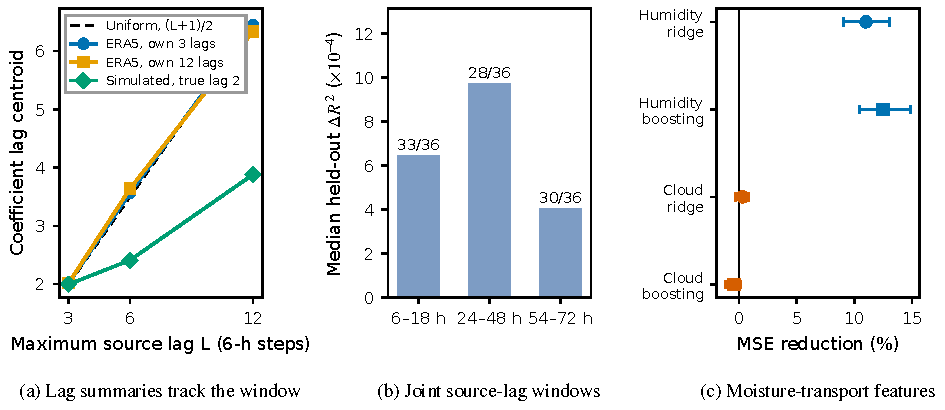
\includegraphics[width=\textwidth]{figures/fig06_timing_transport.pdf}
}\caption{\DIFaddFL{Timing and transport. Lag summaries follow the tested window even when the true lag is short, held-out information is spread over all three lag windows, and moisture-transport features improve humidity but not cloud prediction.}}
\label{fig:timing}
\end{figure}

\DIFadd{Time-aligned path models show that humidity explains only part of the wind--cloud dependence. Among the 20 strong paths, the humidity}\DIFaddend $\rightarrow$\DIFdelbegin \DIFdel{Humidity, Humidity }\DIFdelend \DIFaddbegin \DIFadd{cloud stage given wind improves held-out prediction in 19 (median $\Delta R^2=1.6\times10^{-3}$), the wind}\DIFaddend $\rightarrow$\DIFdelbegin \DIFdel{Cloud Cover and Wind }\DIFdelend \DIFaddbegin \DIFadd{humidity stage in 20 ($5.2\times10^{-4}$) and the direct wind}\DIFaddend $\rightarrow$\DIFdelbegin \DIFdel{Cloud Cover remained concentrated at lag 1, but the mean lag was approximately 5.9-6.3 time steps, and }\DIFdelend \DIFaddbegin \DIFadd{cloud term given the specified intermediate humidity still in 14 ($1.7\times10^{-4}$). With the six physical controls taken before the path source, these counts are 17, 19 and 14 and the median gains shrink to $5.3\times10^{-4}$, $1.0\times10^{-4}$ and $6.1\times10^{-5}$. The earlier mean attenuation of 3.69\% after adding target-region humidity is therefore a coarse summary of a partial, control-sensitive dependence and not an identified mediated fraction (Supplementary Tables~S10 and~S12). Projecting wind and moisture flux onto the source--target direction adds held-out information in 331 and 320 of 396 models, but with small median gains ($\Delta R^2=4.6\times10^{-5}$ and $7.9\times10^{-5}$). In the two Atlantic footprints, transport features reduce the held-out mean squared error of }\DIFaddend the \DIFdelbegin \DIFdel{lag 4-8 range, corresponding to 24-48 hours, accounted for a large fraction.

Humidity mediation tests showed that after controlling for Humidity,Wind $\rightarrow$ Cloud Cover coefficients decreased overall but only modestly. The mean reduction was 0.037 in the all regime and approximately 0.104 and 0.109 in high\_humidity and high\_cloud regimes, respectively}\DIFdelend \DIFaddbegin \DIFadd{6-h humidity change by 11.02\% (95\% interval 9.09--13.10\%) for ridge regression and 12.51\% (10.42--14.87\%) for gradient boosting, whereas the cloud-cover changes are 0.32\% ($-0.30$ to $0.79$\%) and $-0.44$\% ($-1.14$ to $0.16$\%) (Figure~\ref{fig:timing}c). Resolved horizontal transport thus carries information about subsequent humidity, but not enough about cloud, which also depends on vertical motion, stability and microphysics.

}

\subsection{\DIFadd{Independent satellite cloud}}
\label{subsec:ceres_res}

\DIFadd{ERA5 and CERES cloud anomalies agree moderately (Figure~\ref{fig:ceres}a). Over 2017-01-01 to 2023-01-10, the median correlation is 0.758 at the grid scale and 0.763 at the regional scale (range 0.371--0.914), with weakest agreement in polar regions (Supplementary Table~S15); CERES cloud cover is 4.0 percentage points higher on an area-weighted basis. Agreement is the same in 2023-01-11 to 2025-12-31 (0.764 and 0.778), whereas fields requested on the coarse CDS grid had lowered the grid-scale correlation in this segment to 0.612, independent evidence that the regridding route matters}\DIFaddend .

\begin{figure}[htbp]
\centering
\DIFdelbeginFL \DIFdelFL{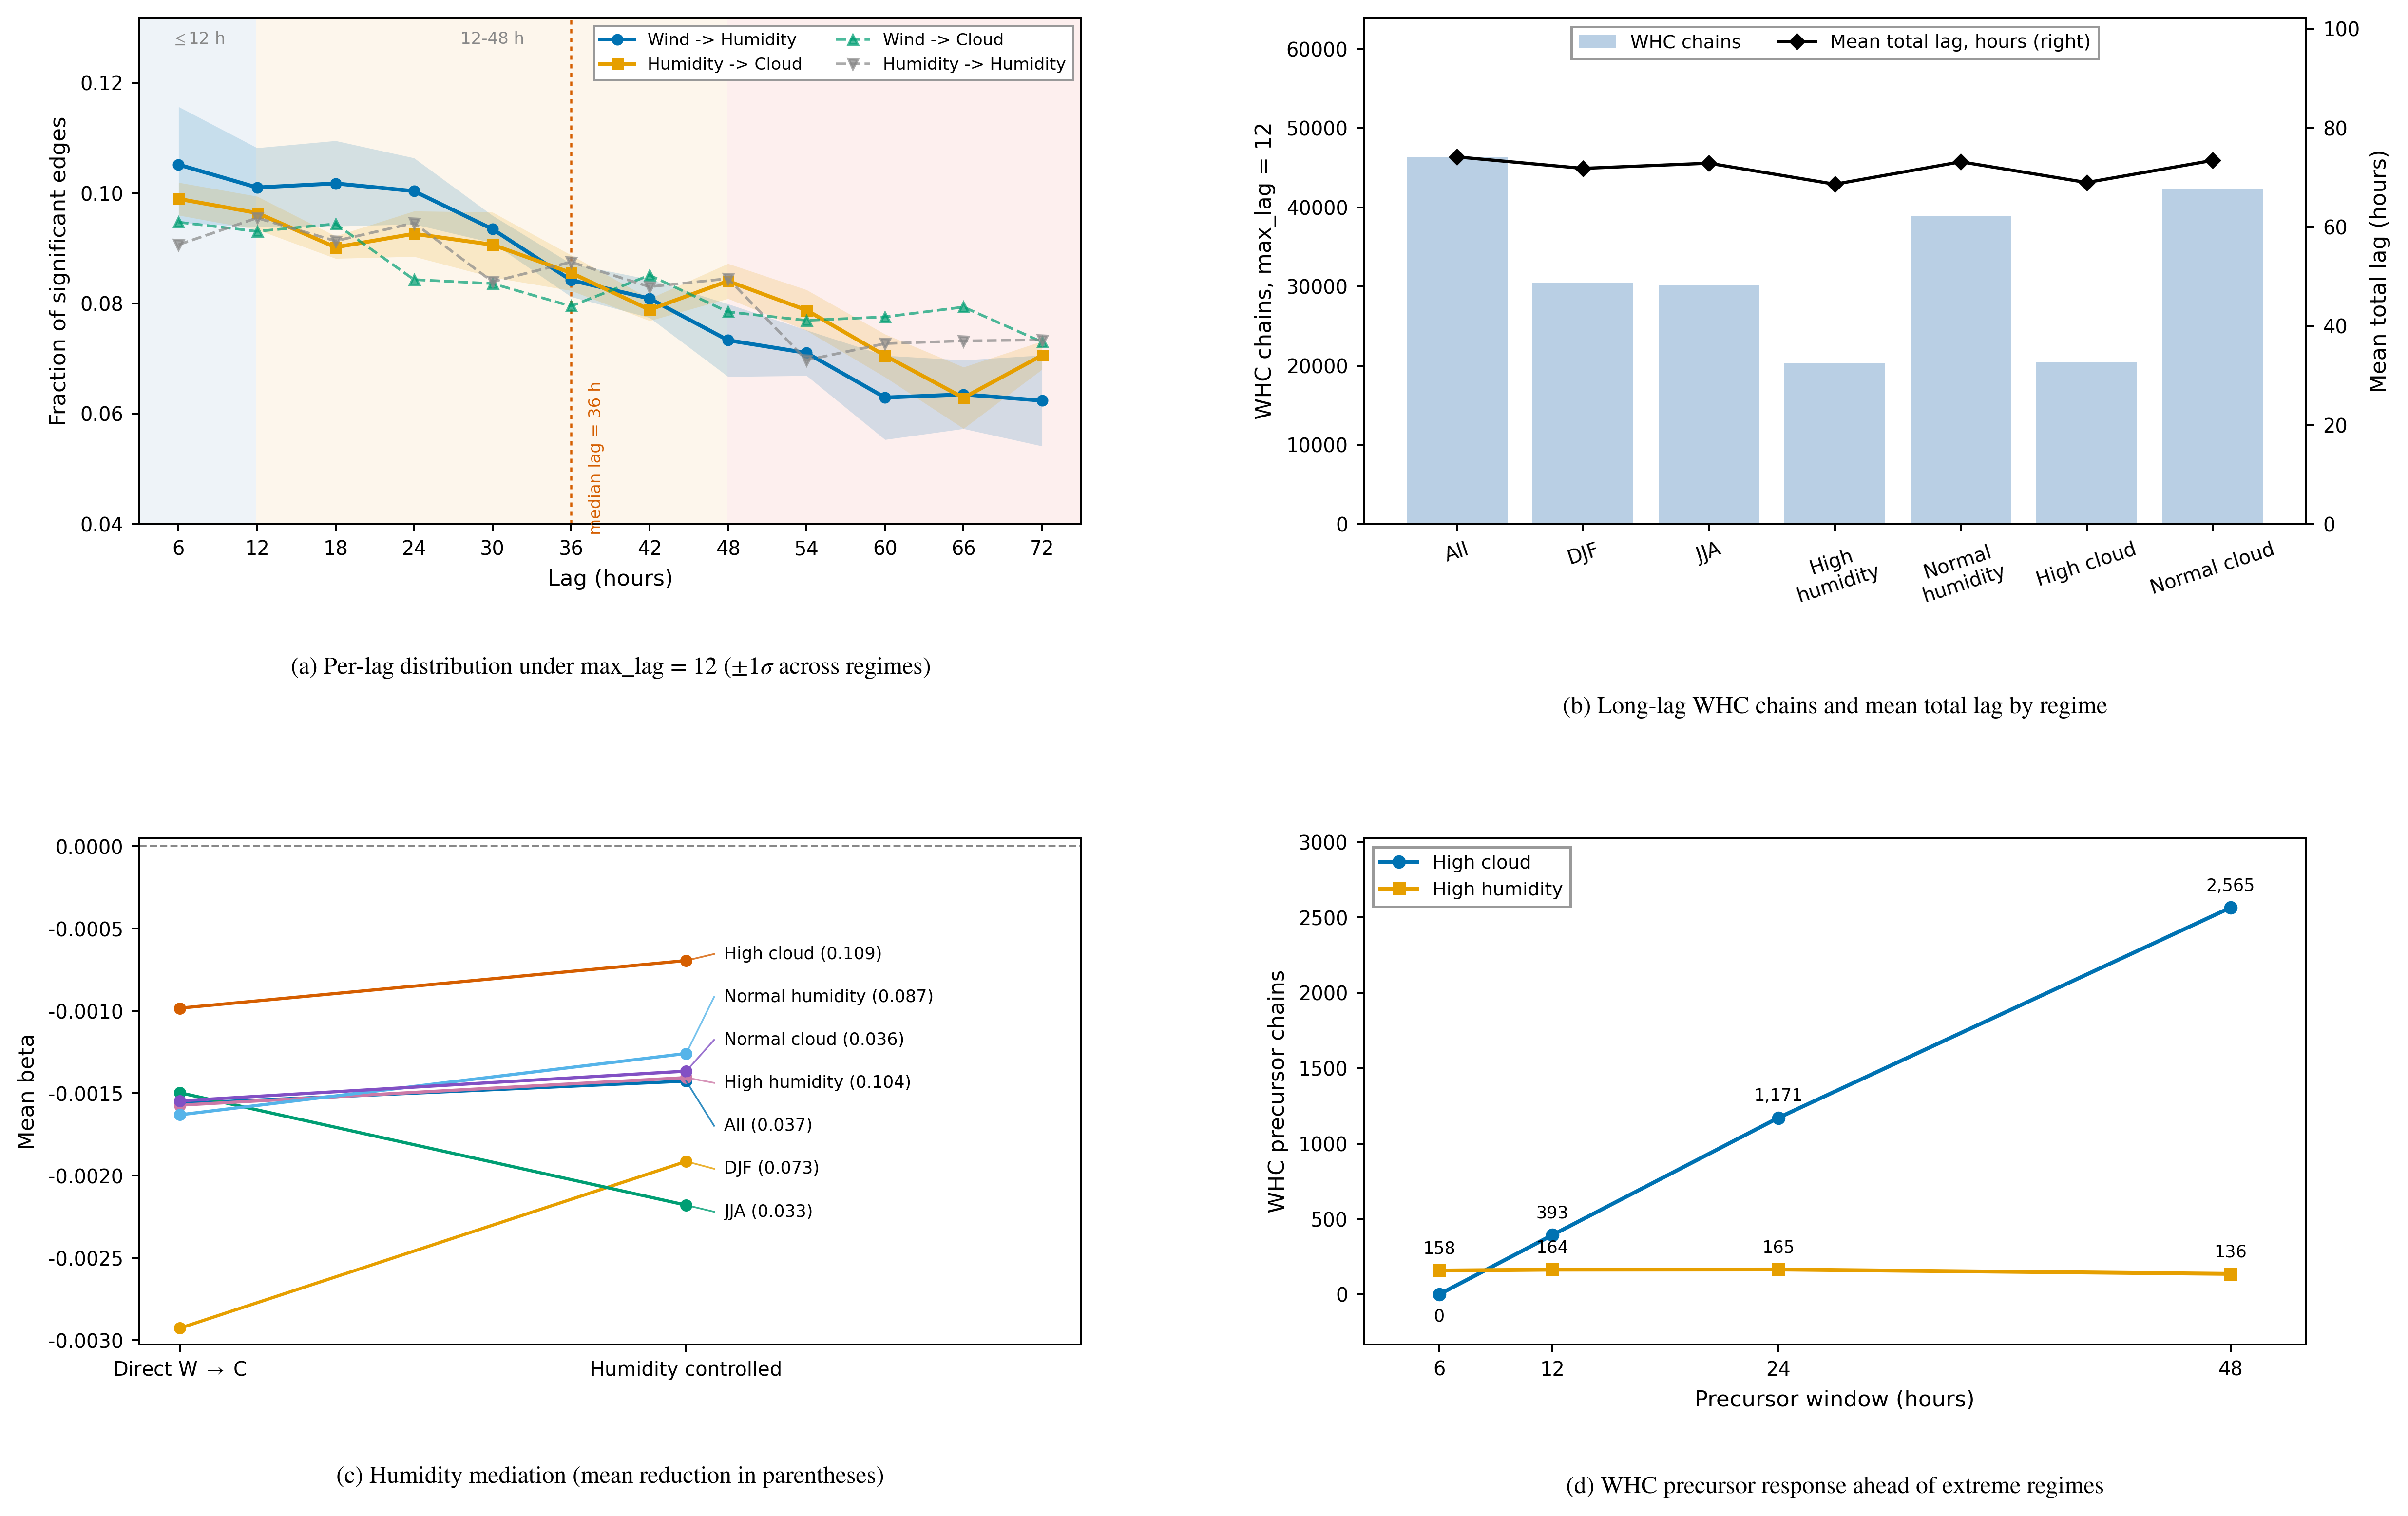
\includegraphics[width=0.98\textwidth]{figures/top_conference/fig06_temporal_mechanism.png}
}\DIFdelendFL \DIFaddbeginFL \DIFaddFL{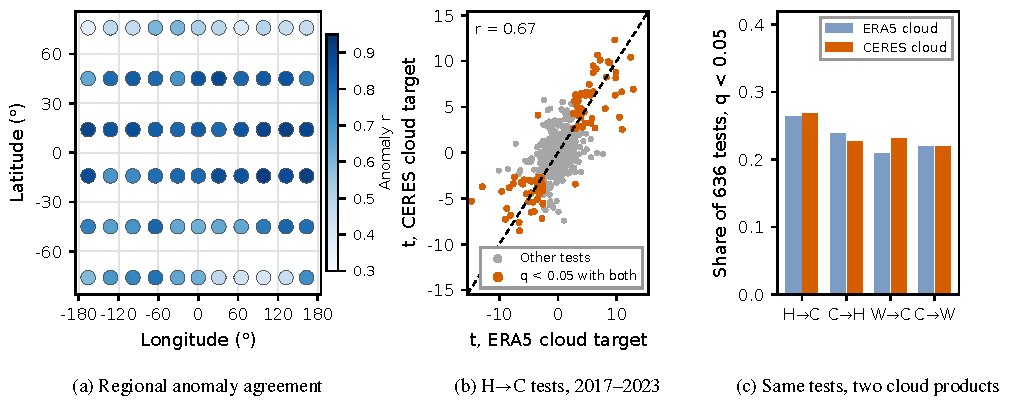
\includegraphics[width=\textwidth]{figures/fig07_ceres.pdf}
}\DIFaddendFL \caption{\DIFdelbeginFL \DIFdelFL{Mechanism boundaries of the pathway: latitude-band structure}\DIFdelendFL \DIFaddbeginFL \DIFaddFL{Satellite cloud substitution. Regional ERA5 and CERES cloud anomalies agree moderately}\DIFaddendFL , \DIFdelbeginFL \DIFdelFL{long-lag behaviour }\DIFdelendFL and humidity\DIFdelbeginFL \DIFdelFL{mediation of Wind }\DIFdelendFL $\rightarrow$\DIFdelbeginFL \DIFdelFL{Cloud Cover}\DIFdelendFL \DIFaddbeginFL \DIFaddFL{cloud tests give similar prevalence and consistent signs with either cloud product}\DIFaddendFL .}
\DIFdelbeginFL %DIFDELCMD < \label{fig:6}
%DIFDELCMD < %%%
\DIFdelendFL \DIFaddbeginFL \label{fig:ceres}
\DIFaddendFL \end{figure}

\DIFaddbegin \DIFadd{Replacing ERA5 cloud by CERES cloud leaves the humidity--cloud dependence intact (Table~\ref{tab:ceres}; Figure~\ref{fig:ceres}b,c). Under full conditioning in 2017--2023, 168 humidity$\rightarrow$cloud tests are significant with ERA5 cloud and 171 with CERES cloud; 94 are significant with both, 92 of them with the same sign, and the $t$-statistics correlate at 0.67 across all 636 tests. Results are similar for the reverse direction and for wind--cloud pairs, with lower $t$-correlations for the latter (0.46--0.51), and they are unchanged with a month $\times$ UTC-hour climatology. The humidity$\rightarrow$cloud dependence is therefore not an artefact of the reanalysis cloud scheme, and it recurs in 2023-01-11 to 2025-12-31, where 109 and 88 tests are significant with ERA5 and CERES cloud and all 51 tests significant with both share the sign ($t$-correlation 0.66). The direction asymmetry, however, is not detected with CERES cloud in this shorter segment (49.4\% of pairs, $p=0.71$, against 53.9\%, $p=0.023$, with ERA5 cloud; Table~\ref{tab:direction}), so the satellite support for the humidity$\rightarrow$cloud orientation rests on 2017--2023.

}

\DIFaddend \begin{table}[htbp]
\centering
\DIFdelbeginFL %DIFDELCMD < \caption{%
{%DIFAUXCMD
\DIFdelFL{Latitude-band WHC chain statistics.}}
%DIFAUXCMD
%DIFDELCMD < \label{tab:13}
%DIFDELCMD < \scriptsize
%DIFDELCMD < \resizebox{\textwidth}{!}{%
%DIFDELCMD < \begin{tabular}{@{}lllll@{}}
%DIFDELCMD < \toprule
%DIFDELCMD < Latitude band & WHC chains & Stable WHC chains & Mean total lag & Mean chain score \\
%DIFDELCMD < \midrule
%DIFDELCMD < tropical & 6,017 & 1,201 & 3.985 & 0.451 \\
%DIFDELCMD < midlatitude & 9,612 & 3,628 & 3.983 & 0.642 \\
%DIFDELCMD < polar & 6,573 & 888 & 3.941 & 0.375 \\
%DIFDELCMD < \bottomrule
%DIFDELCMD < \end{tabular}%
%DIFDELCMD < }
%DIFDELCMD < %%%
\DIFdelendFL \DIFaddbeginFL \caption{\DIFaddFL{Tests with ERA5 and CERES cloud, 2017-01-01 to 2023-01-10.}}
\label{tab:ceres}
\footnotesize
\setlength{\tabcolsep}{2.8pt}
\begin{tabular}{@{}lllrrrl@{}}
\toprule
& \DIFaddFL{Own history }& \multicolumn{4}{c}{\DIFaddFL{Full conditioning}} & \DIFaddFL{Diurnal }\\
\cmidrule(lr){2-2}\cmidrule(lr){3-6}\cmidrule(lr){7-7}
\DIFaddFL{Edge type }& \DIFaddFL{ERA5 / CERES }& \DIFaddFL{ERA5 / CERES }& \DIFaddFL{Both }& \DIFaddFL{Same sign }& \DIFaddFL{$t$ corr. }& \DIFaddFL{ERA5 / CERES }\\
\midrule
\DIFaddFL{$H\rightarrow C$ }& \DIFaddFL{378 / 396 }& \DIFaddFL{168 / 171 }& \DIFaddFL{94 }& \DIFaddFL{92 }& \DIFaddFL{0.67 }& \DIFaddFL{157 / 155 }\\
\DIFaddFL{$C\rightarrow H$ }& \DIFaddFL{412 / 435 }& \DIFaddFL{152 / 144 }& \DIFaddFL{84 }& \DIFaddFL{84 }& \DIFaddFL{0.73 }& \DIFaddFL{138 / 131 }\\
\DIFaddFL{$W\rightarrow C$ }& \DIFaddFL{383 / 388 }& \DIFaddFL{133 / 147 }& \DIFaddFL{56 }& \DIFaddFL{50 }& \DIFaddFL{0.46 }& \DIFaddFL{129 / 140 }\\
\DIFaddFL{$C\rightarrow W$ }& \DIFaddFL{373 / 385 }& \DIFaddFL{139 / 139 }& \DIFaddFL{54 }& \DIFaddFL{53 }& \DIFaddFL{0.51 }& \DIFaddFL{120 / 123 }\\
\bottomrule
\end{tabular}
\DIFaddendFL \end{table}

\DIFdelbegin %DIFDELCMD < \begin{table}[htbp]
%DIFDELCMD < %%%
\DIFdelendFL \DIFaddbeginFL \subsection{\DIFaddFL{Wind--humidity eddy convergence}}
\label{subsec:whec_res}

\DIFaddFL{The pre-specified test supports a WHEC effect on cloud (Figure~\ref{fig:whec}). In midlatitude regions, the frozen WHEC block reduces the held-out cloud-prediction error by 0.456\% in 2019--2023 (HAC $z=10.6$) and by 0.359\% in 2023--2025 ($z=6.8$), against 0.149\% and 0.144\% in the tropics; the midlatitude excess of 0.307 and 0.215 percentage points ($z=6.6$ and 3.8) satisfies E2. The remote-region and placebo versions give midlatitude error reductions between $-0.016$\% and $-0.001$\% ($z$ from $-2.2$ to $-0.2$), so both controls fail E1, and the frozen decision rule classifies the effect as supported in both held-out segments. The effect is not confined to the midlatitudes: polar regions gain 0.501\% and 0.623\%, as much as or more than midlatitude regions. All 22 midlatitude regions gain in 2019--2023 and 20 in 2023--2025.

}

\begin{figure}[htbp]
\DIFaddendFL \centering
\DIFdelbeginFL %DIFDELCMD < \caption{%
{%DIFAUXCMD
\DIFdelFL{Long-lag experiment with max\_lag=12.}}
%DIFAUXCMD
%DIFDELCMD < \label{tab:14}
%DIFDELCMD < \scriptsize
%DIFDELCMD < \resizebox{\textwidth}{!}{%
%DIFDELCMD < \begin{tabular}{@{}llllllll@{}}
%DIFDELCMD < \toprule
%DIFDELCMD < Edge type & Peak lag & Mean lag & Median lag & Lag 1 fraction & Lag 2-3 fraction & Lag 4-8 fraction & Lag 9-12 fraction \\
%DIFDELCMD < \midrule
%DIFDELCMD < Wind $\rightarrow$ Humidity & 1 & 5.89 & 6.0 & 0.103 & 0.200 & 0.433 & 0.263 \\
%DIFDELCMD < Humidity $\rightarrow$ Cloud Cover & 1 & 6.09 & 6.0 & 0.099 & 0.186 & 0.431 & 0.284 \\
%DIFDELCMD < Wind $\rightarrow$ Cloud Cover & 1 & 6.25 & 6.0 & 0.094 & 0.187 & 0.412 & 0.307 \\
%DIFDELCMD < Humidity $\rightarrow$ Humidity & 2 & 6.19 & 6.0 & 0.090 & 0.186 & 0.433 & 0.291 \\
%DIFDELCMD < \bottomrule
%DIFDELCMD < \end{tabular}%
%DIFDELCMD < }
%DIFDELCMD < \end{table}
%DIFDELCMD < %%%
\DIFdelend \DIFaddbegin \DIFadd{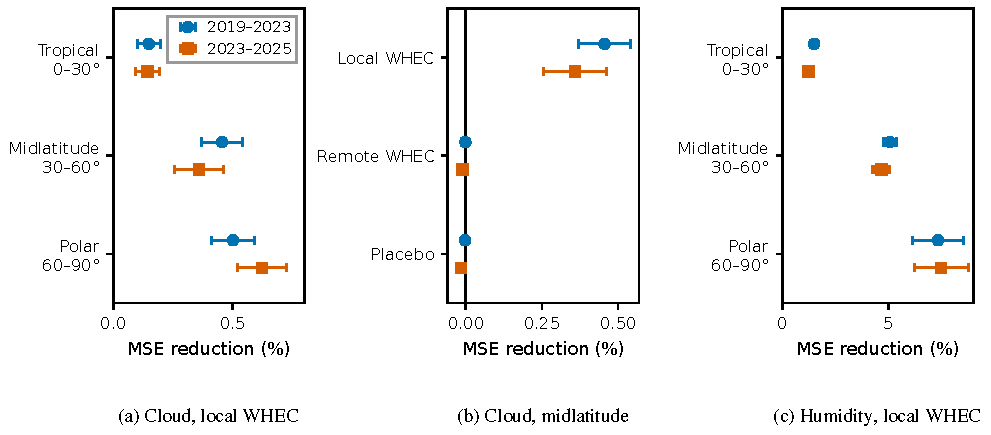
\includegraphics[width=\textwidth]{figures/fig08_whec.pdf}
}\caption{\DIFadd{Wind--humidity eddy convergence test. Frozen 1979--2018 gains in held-out cloud (a) and humidity (c) prediction by latitude band, and midlatitude cloud gains of the local index and its two controls (b), with 95\% HAC intervals.}}
\label{fig:whec}
\end{figure}

\DIFaddend 

\DIFaddbegin \DIFadd{Lag-specific tests agree (Table~\ref{tab:whec}). Of the 198 local cloud hypotheses, 168 pass the screen and 139 are confirmed, against one in each control family; 86 replicate in 2019--2023 and 66 in 2023--2025, whereas 1 of 59 unconfirmed local hypotheses does so in each segment. All 54 confirmed coefficients at 6~h are positive and 39 of the 44 at 12~h are negative, so cloud follows a recent increase in eddy convergence rather than its level. For humidity, the secondary target, the WHEC block reduces the midlatitude error by 5.07\% and 4.66\%, 3.4 and 3.8 times the tropical gain, as expected from the moisture budget. With CERES cloud as both predictor and outcome in refits on 2017--2023 and 2023--2025, 64 and 41 of the 198 local cloud hypotheses keep their discovery sign at $q<0.05$, against at most 6 for the control families, although midlatitude support with CERES cloud is weak in the shorter second segment (6 of 66). The gains are small: a reduction of about 0.4\% in the cloud-prediction error matches the non-significant cloud change in the two-footprint transport experiment and becomes detectable only when 22 regions are pooled.

}

\DIFaddend \begin{table}[htbp]
\centering
\DIFdelbeginFL %DIFDELCMD < \caption{%
{%DIFAUXCMD
\DIFdelFL{Humidity mediation test for Wind $\rightarrow$ Cloud Cover.}}
%DIFAUXCMD
%DIFDELCMD < \label{tab:15}
%DIFDELCMD < %%%
\DIFdelendFL \DIFaddbeginFL \caption{\DIFaddFL{Wind--humidity eddy convergence test, 198 lag-specific hypotheses per family and target; families use the local WHEC, the WHEC of a remote region in the same latitude band, or the time-shifted placebo. Replicated: confirmed and same-sign replication $q<0.05$; unconfirmed: the same rule applied to hypotheses that failed Stage~1 or~2; CERES: discovery sign and $q<0.05$ in refits with CERES cloud.}}
\label{tab:whec}
\DIFaddendFL \scriptsize
\DIFdelbeginFL %DIFDELCMD < \resizebox{\textwidth}{!}{%
%DIFDELCMD < \begin{tabular}{@{}lllllll@{}}
%DIFDELCMD < \toprule
%DIFDELCMD < Regime & WC edges & Mean direct beta & Mean beta after controlling Humidity & Mean reduction & Reduction > 30\% & Reduction > 50\% \\
%DIFDELCMD < \midrule
%DIFDELCMD < all & 520 & -0.00156 & -0.00143 & 0.0369 & 0.206 & 0.117 \\
%DIFDELCMD < DJF & 436 & -0.00293 & -0.00191 & 0.0729 & 0.211 & 0.108 \\
%DIFDELCMD < JJA & 482 & -0.00150 & -0.00218 & 0.0330 & 0.199 & 0.100 \\
%DIFDELCMD < high\_humidity & 429 & -0.00157 & -0.00140 & 0.1045 & 0.182 & 0.091 \\
%DIFDELCMD < normal\_humidity & 492 & -0.00163 & -0.00126 & 0.0873 & 0.215 & 0.118 \\
%DIFDELCMD < high\_cloud & 391 & -0.00098 & -0.00069 & 0.1090 & 0.192 & 0.079 \\
%DIFDELCMD < normal\_cloud & 510 & -0.00155 & -0.00137 & 0.0358 & 0.198 & 0.102 \\
%DIFDELCMD < \bottomrule
%DIFDELCMD < \end{tabular}%
%DIFDELCMD < }
%DIFDELCMD < %%%
\DIFdelendFL \DIFaddbeginFL \setlength{\tabcolsep}{3.5pt}
\begin{tabular}{@{}llrrrrrrrr@{}}
\toprule
& & & & \multicolumn{2}{c}{\DIFaddFL{Replicated}} & \multicolumn{2}{c}{\DIFaddFL{Unconfirmed}} & \multicolumn{2}{c}{\DIFaddFL{CERES}} \\
\cmidrule(lr){5-6}\cmidrule(lr){7-8}\cmidrule(lr){9-10}
\DIFaddFL{Family }& \DIFaddFL{Target }& \DIFaddFL{Screened }& \DIFaddFL{Confirmed }& \DIFaddFL{2019--23 }& \DIFaddFL{2023--25 }& \DIFaddFL{2019--23 }& \DIFaddFL{2023--25 }& \DIFaddFL{2017--23 }& \DIFaddFL{2023--25 }\\
\midrule
\DIFaddFL{Local }& \DIFaddFL{Cloud }& \DIFaddFL{168 }& \DIFaddFL{139 }& \DIFaddFL{86 }& \DIFaddFL{66 }& \DIFaddFL{1 }& \DIFaddFL{1 }& \DIFaddFL{64 }& \DIFaddFL{41 }\\
 & \DIFaddFL{Humidity }& \DIFaddFL{189 }& \DIFaddFL{178 }& \DIFaddFL{139 }& \DIFaddFL{141 }& \DIFaddFL{2 }& \DIFaddFL{3 }& \DIFaddFL{-- }& \DIFaddFL{-- }\\
\DIFaddFL{Remote }& \DIFaddFL{Cloud }& \DIFaddFL{47 }& \DIFaddFL{1 }& \DIFaddFL{0 }& \DIFaddFL{0 }& \DIFaddFL{0 }& \DIFaddFL{2 }& \DIFaddFL{0 }& \DIFaddFL{0 }\\
 & \DIFaddFL{Humidity }& \DIFaddFL{21 }& \DIFaddFL{1 }& \DIFaddFL{0 }& \DIFaddFL{0 }& \DIFaddFL{0 }& \DIFaddFL{0 }& \DIFaddFL{-- }& \DIFaddFL{-- }\\
\DIFaddFL{Placebo }& \DIFaddFL{Cloud }& \DIFaddFL{1 }& \DIFaddFL{1 }& \DIFaddFL{0 }& \DIFaddFL{1 }& \DIFaddFL{0 }& \DIFaddFL{0 }& \DIFaddFL{6 }& \DIFaddFL{0 }\\
 & \DIFaddFL{Humidity }& \DIFaddFL{1 }& \DIFaddFL{0 }& \DIFaddFL{-- }& \DIFaddFL{-- }& \DIFaddFL{0 }& \DIFaddFL{0 }& \DIFaddFL{-- }& \DIFaddFL{-- }\\
\bottomrule
\end{tabular}
\DIFaddendFL \end{table}

\DIFdelbegin \subsection{\DIFdel{Multivariable adjustment and effect-size analysis}}
%DIFAUXCMD
\addtocounter{subsection}{-1}%DIFAUXCMD
\DIFdelend \DIFaddbegin \subsection{\DIFadd{Comparison with existing methods}}
\label{subsec:bench_res}

\DIFaddend 

\DIFdelbegin \DIFdel{Controlling the complete recent multivariate state of }\DIFdelend \DIFaddbegin \DIFadd{Table~\ref{tab:benchmark} summarizes the benchmarks. In }\DIFaddend the \DIFdelbegin \DIFdel{target region reduced
the number of all-regime significant edge--lag hypotheses from 2, 218 to 2, 163, but retained 1, 920 of the original discoveries. Wind $\rightarrow$ Humidity,
Humidity $\rightarrow$ Cloud Cover and Wind $\rightarrow$ Cloud Cover retained
439/503, 407/488 and 428/520 original significant hypotheses, corresponding to recovery fractions of 0.873, 0.834 and 0.823.

The adjusted graph still contained
3,624 WHC chains , compared with 3, 746 in the principal model. The core pathway
is therefore not removed by controlling recent temperature, humidity, wind and cloud history in the target region.
}%DIFDELCMD < 

%DIFDELCMD < %%%
\DIFdel{The median effects across all significant hypotheses were statistically clear
but individually small. Under multivariable adjustment, median absolute
standardized coefficients were 0.0138, 0.0207 and 0.0176 for WH, HC and WC, while median partial $R^2$ values were 0.00117, 0.00090 and 0.00084. This
distinguishes the widespread graph-level recurrence of the pathway from the magnitude of any single edge. In contrast, the ten strongest stable edges per
pathway had median absolute coefficients of 0.195}\DIFdelend \DIFaddbegin \DIFadd{known-structure systems, all-history regression and PCMCI are comparably accurate and both far exceed own-history regression, while HAC inference lowers F1 by at most 0.02 relative to OLS (Supplementary Table~S13). In the regime-switching benchmark, hidden-state Regime-PCMCI raises F1 from 0.610 for pooled PCMCI to 0.826 and recovers the state sequence with mean accuracy 0.846, but it is variable across replicates (standard deviation 0.237) and about 750 times slower; methods given the true state masks reach 0.936}\DIFaddend --0\DIFdelbegin \DIFdel{.328 and median partial
$R^2$ of 0.035}\DIFdelend \DIFaddbegin \DIFadd{.983. Regime-PCMCI therefore provides a capability that our prescribed regimes do not, namely learning unknown states. In lattice benchmarks, CaStLe reaches F1 of 0.971}\DIFaddend --0\DIFdelbegin \DIFdel{.042. All 30 of these selected edges had year-block bootstrap
95\% intervals excluding zero, with median sign consistency of 1.0 across the 47 annual blocks}\DIFdelend \DIFaddbegin \DIFadd{.976 when spatial structure is homogeneous but drops to 0.780--0.786, with precision of about 0.65, when it is heterogeneous, where local estimators retain precision above 0.95. Neither benchmark makes Causal WeatherGraph a more accurate identification algorithm; its contribution is the verification layer of confirmation, replication and negative controls, which these methods do not provide}\DIFaddend .

\begin{table}[htbp]
\centering
\DIFdelbeginFL %DIFDELCMD < \caption{%%%
\DIFdelFL{All-regime multivariable-control and effect-size summary.}%DIFDELCMD < \MBLOCKRIGHTBRACE
%DIFDELCMD < \label{tab:effect_size}
%DIFDELCMD < \scriptsize
%DIFDELCMD < \resizebox{\textwidth}{!}{%
%DIFDELCMD < \begin{tabular}{@{}llllllll@{}}
%DIFDELCMD < \toprule
%DIFDELCMD < Edge type & Principal significant & Adjusted significant & Original retained & Recovery & Median $|\beta|$ & Median partial $R^2$ & Top-edge block CI exclusion \\
%DIFDELCMD < \midrule
%DIFDELCMD < Wind $\rightarrow$ Humidity & 503 & 490 & 439 & 0.873 & 0.0138 & 0.00117 & 10/10 \\
%DIFDELCMD < Humidity $\rightarrow$ Cloud Cover & 488 & 483 & 407 & 0.834 & 0.0207 & 0.00090 & 10/10 \\
%DIFDELCMD < Wind $\rightarrow$ Cloud Cover & 520 & 487 & 428 & 0.823 & 0.0176 & 0.00084 & 10/10 \\
%DIFDELCMD < \bottomrule
%DIFDELCMD < \end{tabular}%
%DIFDELCMD < }
%DIFDELCMD < \end{table}
%DIFDELCMD < %%%
\DIFdelend \DIFaddbegin \caption{\DIFadd{Benchmarks with known structure. Panel A: mean F1 over 50 replicates and runtime per fit; Panel B: regime-switching system, 20 replicates; Panel C: lattice systems, mean F1 over 25 replicates.}}
\label{tab:benchmark}
\footnotesize
\setlength{\tabcolsep}{3.5pt}
\begin{tabular}{@{}lrrrrrr@{}}
\toprule
\multicolumn{7}{@{}l}{\textit{\DIFadd{A. Six-variable systems}}} \\
\DIFadd{Method }& \shortstack[r]{\DIFadd{Weak}\\\DIFadd{AR}} & \shortstack[r]{\DIFadd{Strong}\\\DIFadd{AR}} & \shortstack[r]{\DIFadd{Observed}\\\DIFadd{driver}} & \shortstack[r]{\DIFadd{Hidden}\\\DIFadd{driver}} & \shortstack[r]{\DIFadd{Regime}\\\DIFadd{switch}} & \DIFadd{s/fit }\\
\midrule
\DIFadd{Own-history OLS }& \DIFadd{0.654 }& \DIFadd{0.158 }& \DIFadd{0.143 }& \DIFadd{0.143 }& \DIFadd{0.816 }& \DIFadd{0.07 }\\
\DIFadd{Own-history HAC }& \DIFadd{0.639 }& \DIFadd{0.157 }& \DIFadd{0.142 }& \DIFadd{0.142 }& \DIFadd{0.801 }& \DIFadd{0.07 }\\
\DIFadd{All-history OLS }& \DIFadd{0.986 }& \DIFadd{0.970 }& \DIFadd{0.974 }& \DIFadd{0.259 }& \DIFadd{0.976 }& \DIFadd{0.22 }\\
\DIFadd{All-history HAC }& \DIFadd{0.976 }& \DIFadd{0.966 }& \DIFadd{0.965 }& \DIFadd{0.258 }& \DIFadd{0.957 }& \DIFadd{0.22 }\\
\DIFadd{PCMCI }& \DIFadd{0.978 }& \DIFadd{0.973 }& \DIFadd{0.956 }& \DIFadd{0.252 }& \DIFadd{0.976 }& \DIFadd{0.48 }\\
\bottomrule
\end{tabular}

\DIFaddend 

\DIFdelbegin \subsection{\DIFdel{PCMCI confirmation on the recent-period sample}}
%DIFAUXCMD
\addtocounter{subsection}{-1}%DIFAUXCMD
\DIFdelend \DIFaddbegin \vspace{6pt}
\begin{tabular}{@{}llrrlrr@{}}
\toprule
\multicolumn{7}{@{}l}{\textit{\DIFadd{B. Regime-switching system}}} \\
\DIFadd{Method }& \DIFadd{Given }& \DIFadd{Precision }& \DIFadd{Recall }& \DIFadd{F1 (SD) }& \DIFadd{s/fit }& \DIFadd{Peak MiB }\\
\midrule
\DIFadd{Pooled PCMCI }& \DIFadd{none }& \DIFadd{0.473 }& \DIFadd{0.871 }& \DIFadd{0.610 (0.040) }& \DIFadd{0.24 }& \DIFadd{181 }\\
\DIFadd{Regime-PCMCI }& \DIFadd{state count }& \DIFadd{0.859 }& \DIFadd{0.871 }& \DIFadd{0.826 (0.237) }& \DIFadd{179.66 }& \DIFadd{862 }\\
\DIFadd{Own-history OLS }& \DIFadd{true masks }& \DIFadd{0.889 }& \DIFadd{0.996 }& \DIFadd{0.936 (0.047) }& \DIFadd{0.10 }& \DIFadd{181 }\\
\DIFadd{All-history HAC }& \DIFadd{true masks }& \DIFadd{0.893 }& \DIFadd{0.996 }& \DIFadd{0.936 (0.065) }& \DIFadd{0.19 }& \DIFadd{182 }\\
\DIFadd{All-history OLS }& \DIFadd{true masks }& \DIFadd{0.966 }& \DIFadd{0.996 }& \DIFadd{0.978 (0.035) }& \DIFadd{0.19 }& \DIFadd{182 }\\
\DIFadd{PCMCI }& \DIFadd{true masks }& \DIFadd{0.973 }& \DIFadd{0.996 }& \DIFadd{0.983 (0.025) }& \DIFadd{0.31 }& \DIFadd{182 }\\
\bottomrule
\end{tabular}

\DIFaddend 

\DIFdelbegin \DIFdel{PCMCI was run for 60 top all-regime stable Granger-style edges using the 2019--2025 data segment at 6-hour resolution. After conditional-independence
testing and Benjamini--Hochberg correction, }\DIFdelend \DIFaddbegin \vspace{6pt}
\begin{tabular}{@{}lrrrr@{}}
\toprule
\multicolumn{5}{@{}l}{\textit{\DIFadd{C. Lattice systems}}} \\
& \multicolumn{2}{c}{\DIFadd{Homogeneous}} & \multicolumn{2}{c}{\DIFadd{Heterogeneous}} \\
\cmidrule(lr){2-3}\cmidrule(lr){4-5}
\DIFadd{Method }& \DIFadd{$6\times6$ }& \DIFadd{$10\times10$ }& \DIFadd{$6\times6$ }& \DIFadd{$10\times10$ }\\
\midrule
\DIFadd{CaStLe (official) }& \DIFadd{0.971 }& \DIFadd{0.976 }& \DIFadd{0.780 }& \DIFadd{0.786 }\\
\DIFadd{Local own-history OLS }& \DIFadd{0.764 }& \DIFadd{0.758 }& \DIFadd{0.720 }& \DIFadd{0.757 }\\
\DIFadd{Local multivariable OLS }& \DIFadd{0.724 }& \DIFadd{0.717 }& \DIFadd{0.680 }& \DIFadd{0.727 }\\
\DIFadd{Local PCMCI }& \DIFadd{0.739 }& \DIFadd{0.735 }& \DIFadd{0.698 }& \DIFadd{0.736 }\\
\bottomrule
\end{tabular}
\end{table}

\DIFadd{The framework scales to the full problem on a workstation (Intel Core Ultra 9 275HX, 64~GB memory). Screening the }\DIFaddend 18\DIFdelbegin \DIFdel{of 20 Wind $\rightarrow$
Humidity edges, 16 of 20 Humidity $\rightarrow$ Cloud Cover edges and 16 of 20
Wind $\rightarrow$ Cloud Cover edges remained significant. Mean absolute PCMCI
partial correlations were 0.0867}\DIFdelend ,\DIFdelbegin \DIFdel{0.0426 and 0.0815, respectively. This
confirmation does not remove the observational assumptions of PCMCI, but it shows that most strongest stable edges survive a separate conditional-
independence discovery procedure in }\DIFdelend \DIFaddbegin \DIFadd{018 regime tests takes 157~s, fitting and testing the dense VAR(3) on 58,437 discovery responses with 264 outcomes takes 29~s, and }\DIFaddend the \DIFdelbegin \DIFdel{recent historical period. }\DIFdelend \DIFaddbegin \DIFadd{complete three-stage analysis over both candidate sets and all segments takes 118~s with a peak memory of 2.4~GB.

}\DIFaddend 

\DIFdelbegin %DIFDELCMD < \begin{table}[htbp]
%DIFDELCMD < \centering
%DIFDELCMD < \caption{%%%
\DIFdelFL{PCMCI validation }\DIFdelendFL \DIFaddbeginFL \subsection{\DIFaddFL{Robustness of the screening stage}}
\label{subsec:robust_res}

\DIFaddFL{The screening stage is stable under perturbation, but this stability mainly reflects its saturation. With $k=2$, 857 }\DIFaddendFL of \DIFdelbeginFL \DIFdelFL{top stable all-regime edges over 2019--2025.}%DIFDELCMD < \MBLOCKRIGHTBRACE
%DIFDELCMD < \label{tab:16}
%DIFDELCMD < \scriptsize
%DIFDELCMD < \resizebox{\textwidth}{!}{%
%DIFDELCMD < \begin{tabular}{@{}llllll@{}}
%DIFDELCMD < \toprule
%DIFDELCMD < Edge type & Granger top edges & PCMCI confirmed & Confirmed ratio & Mean absolute partial correlation & Status \\
%DIFDELCMD < \midrule
%DIFDELCMD < Wind $\rightarrow$ Humidity & 20 & 18 & 0.900 & 0.0867 & confirmed \\
%DIFDELCMD < Humidity $\rightarrow$ Cloud Cover & 20 & 16 & 0.800 & 0.0426 & confirmed \\
%DIFDELCMD < Wind $\rightarrow$ Cloud Cover & 20 & 16 & 0.800 & 0.0815 & confirmed \\
%DIFDELCMD < \bottomrule
%DIFDELCMD < \end{tabular}%
%DIFDELCMD < }
%DIFDELCMD < \end{table}
%DIFDELCMD < %%%
\DIFdelend \DIFaddbegin \DIFadd{858 candidates are significant at some lag; expanding the neighbourhood to $k=4$, 6 and 8 recovers all 857 edges, different preprocessing choices preserve 85--88\% of lag-resolved chains, and alternative regionalizations and historical periods give similar significance rates (Supplementary Tables~S2--S5). Bootstrap resampling of the lagged calendar design with block lengths of 64, 128 and 256 steps gives nearly identical coefficient intervals across block lengths for twelve fixed edge--regime models (Supplementary Table~S8). These analyses show that the screened graph is reproducible, not that its structure is specific; specificity and replication are assessed in Sections~\ref{subsec:three_res} and~\ref{subsec:dir_res}.

}\DIFaddend 

\section{Discussion and Limitations}
\label{sec:discussion}

\DIFdelbegin \subsection{\DIFdel{Interpretation and physical implications}}
%DIFAUXCMD
\addtocounter{subsection}{-1}%DIFAUXCMD
%DIFDELCMD < 

%DIFDELCMD < %%%
\DIFdel{The results support a cautious but clear interpretation: in 6-hourly global reanalysis data from 1979 to 2025, Wind $\rightarrow$ Humidity $\rightarrow$ Cloud Cover appears as a stable, non-random and reproducible lagged directed dependency pathway across regimes and historical periods. The pathway is enriched in the physical candidate graph, remains approximately 1.7-fold enriched under variable-preserved random controls, survives block bootstrap and historical-period splits, and is robust to preprocessing and region-aggregation choices. }\DIFdelend \DIFaddbegin \subsection{\DIFadd{What replicates and what does not}}

\DIFaddend 

\DIFdelbegin \DIFdel{The most important mechanistic signal is the midlatitude enhancement. Midlatitude regions have more chains, more stable chains and higher mean chain scores than tropical or polar regions. This pattern is consistent with synoptic-scale moisture advection, frontal lifting and cloud response. Causal WeatherGraph therefore provides more than a correlation graph: it links statistical dependency, spatial organization and physical interpretation in a regional evidence framework.
}\DIFdelend \DIFaddbegin \DIFadd{The three stages answer different questions. Screening asks whether a source lag adds information beyond the target's own history, which is true of almost every physically motivated candidate in a strongly coupled reanalysis. Confirmation asks whether the information survives conditioning on all other observed histories, which removes 29\% of the screened hypotheses and reverses the sign of many others. Replication asks whether confirmed dependencies recur in years not used for any modelling decision, which roughly half of them do in 2019--2023, about five times as often as unconfirmed hypotheses under the same rule, and 43\% do in 2023--2025. The replicated set of 760 conditional dependencies, which is concentrated at mid and high latitudes and in zonally adjacent regions and whose held-out information is not confined to the shortest lags, is the principal empirical output of our framework.

}\DIFaddend 

\DIFdelbegin \DIFdel{The regime-aware results indicate that atmospheric dependency graphs should not be treated as static structures. In DJF, the Wind $\rightarrow$ Humidity fraction and chain score are relatively high, suggesting that wind-to-moisture lagged dependence is stronger under winter conditions. Under high-humidity and high-cloud states, chain counts are not necessarily largest, but chain scores and mediation reductions tend to be stronger. Regime changes therefore affect notonly the number of edges but also pathway intensity and interpretation.
}%DIFDELCMD < 

%DIFDELCMD < %%%
\DIFdel{The multivariable and effect-size analyses sharpen this interpretation. Most
all-regime discoveries and nearly all core pathway structure remain after
controlling the recent four-variable state of the target region,and PCMCI
confirms 80--90\% of the selected top stable edges in 2019--2025. At the same
time, median partial $R^2$ values across all significant core edgesare below
0.002. The result is therefore a distributed, recurrent graph-level signal
rather than a claim that every individual atmospheric edge has a large effect. The strongest stable edges form a smaller subset with materially larger
standardized coefficients, partial $R^2$ and year-block consistency. }%DIFDELCMD < 

%DIFDELCMD < %%%
\DIFdel{Several boundaries are essential. First, all results are based on observational reanalysis data andcannot replace intervention experiments.

A significant edge means that a lagged source term statistically increases explanatory power for a target, not that intervening on wind would necessarily change humidity and then cloud cover. Second, atmospheric variables have strong autocorrelation, common weather-system forcing and spatial-neighbour coupling. This is especially important for humidity and cloud cover, where reverse and future-to-past controls remain strong. Third, the high significant ratio of }\DIFdelend \DIFaddbegin \DIFadd{Several properties that a screening-based description of the pathway suggests do not survive. Chain counts are not enriched relative to }\DIFaddend distance-matched random \DIFdelbegin \DIFdel{edges shows that part of the dependency structure arises from spatial-neighbour background. Fourth, humidity mediation explains only part of Wind }\DIFdelend \DIFaddbegin \DIFadd{candidates, so the abundance of wind--humidity--cloud chains reflects the density of a spatially coherent background. The wind$\rightarrow$humidity orientation is imposed by the candidate list rather than supported by the data. The mean summed lag of about 24~h is fixed by the search window. A globally pooled DJF regime mixes opposite local seasons, and cloud-state differences found in the discovery period do not replicate. Humidity remains a partial and control-sensitive channel for wind--cloud dependence rather than an identified mediator.

}

\subsection{\DIFadd{Physical interpretation}}

\DIFadd{The most robust directional result, a modest asymmetry favouring humidity}\DIFaddend $\rightarrow$\DIFdelbegin \DIFdel{Cloud Cover, so the WHC pathway should be described as an important channel , not as the only channel. }\DIFdelend \DIFaddbegin \DIFadd{cloud over cloud$\rightarrow$humidity under full conditioning, is consistent with the role of moisture as a cloud-controlling factor \mbox{%DIFAUXCMD
\citep{Andersen2023CloudSensitivities}}\hskip0pt%DIFAUXCMD
; that it persists with satellite cloud argues against an artefact of the reanalysis cloud scheme. The symmetric wind--humidity dependence is consistent with both variables responding to the same synoptic systems: scalar wind speed measures circulation intensity rather than transport, and only the projected moisture flux carries directional transport information, which adds little beyond scalar wind at the regional scale. The hemispheric difference in seasonal modulation plausibly reflects hemispheric differences in storm tracks, which depend on topography and ocean energy transport \mbox{%DIFAUXCMD
\citep{Shaw2022Stormier} }\hskip0pt%DIFAUXCMD
and which a global DJF average conflates. The eddy-convergence result qualifies the transport picture. The covariance of wind and humidity anomalies, which no linear model of regional anomalies represents, carries information about cloud six hours later beyond the dense autoregression and the linear transport terms, and more outside the tropics than inside them. This pattern is consistent with the link between extratropical cloud water and moisture convergence \mbox{%DIFAUXCMD
\citep{McCoy2022Extratropical} }\hskip0pt%DIFAUXCMD
and with cloud formation in the ascending moist airstreams of cyclones \mbox{%DIFAUXCMD
\citep{Heitmann2024WCB}}\hskip0pt%DIFAUXCMD
, and the positive coefficient at 6~h followed by a negative one at 12~h indicates a response to a recent increase in eddy moisture import. The cloud gains nonetheless remain small, and both the transport experiment and the eddy index show that horizontal moisture transport at 850~hPa explains little of the cloud variability, which also depends on vertical motion, stability and microphysics \mbox{%DIFAUXCMD
\citep{WilsonKemsley2024HighCloud}}\hskip0pt%DIFAUXCMD
.

}\DIFaddend 

\DIFdelbegin \DIFdel{These boundaries strengthen rather than weaken the contribution. Causal WeatherGraph offers a reproducible workflow: restrict the search space with physically interpretable candidate edges, compare graph structures under atmospheric regimes, and use layered controls and robustness tests to check whether a pathway still holds. For atmospheric research that seeks mechanistic interpretation in addition to forecast skill, this framework provides a scalable template for analysing variable propagation. }\DIFdelend \DIFaddbegin \subsection{\DIFadd{Implications for information sciences}}

\DIFaddend 

\DIFdelbegin \DIFdel{From an information-science perspective, the same design pattern --- }\DIFdelend \DIFaddbegin \DIFadd{Three lessons apply beyond the atmosphere. First, single-stage screening with own-history controls is a recall device, not a discovery procedure: in strongly coupled systems it reports indirect and common-driver dependencies with high confidence, and their signs are unreliable. Second, verification of a discovered graph requires information the discovery did not use: held-out periods with frozen procedures and a negative-control family make replication rates interpretable, whereas high overlap among nearly saturated graphs does not. Third, data provenance is part of the inference: a change of acquisition route within the record altered the noise level, the agreement with an independent product and even the apparent direction of a dependence. These design elements, namely }\DIFaddend domain-constrained \DIFdelbegin \DIFdel{candidate generation to control the hypothesis space, regime-conditioned estimation to expose state-dependent structure, and a layered chain of matched nulls, falsification tests and confirmatory re-estimation to control the quality of discovered structure --- is not specific to the atmosphere. It applies wherever directed lagged dependencies must be extracted from large, autocorrelated and partially confounded }\DIFdelend \DIFaddbegin \DIFadd{candidates, full conditioning, held-out replication with negative controls and provenance checks, transfer to other large }\DIFaddend spatio-temporal records \DIFdelbegin \DIFdel{, including trafficand mobility networks, energysystems, hydrology, air quality }\DIFdelend \DIFaddbegin \DIFadd{such as traffic, energy, hydrological }\DIFaddend and epidemiological surveillance \DIFaddbegin \DIFadd{data}\DIFaddend .

\subsection{Limitations and future directions}

Our \DIFdelbegin \DIFdel{study has four main limitations}\DIFdelend \DIFaddbegin \DIFadd{conclusions are bounded in five ways}\DIFaddend . First, \DIFdelbegin \DIFdel{it uses observational reanalysisdata and does not provide interventional causal proof. Granger-style and PCMCI-significant edges remain conditional observational dependencies. Second, although monthly climatology was removed and multiple preprocessing robustness tests were performed, strong autocorrelation, common weather systems and spatial smoothing may still affect edge significance}\DIFdelend \DIFaddbegin \DIFadd{all real-data results are conditional linear predictive dependencies in an observational reanalysis; the hidden-driver simulations show that no method we tested recovers structure when relevant drivers are unobserved, and the six physical controls do not form a complete adjustment set. Second, HAC-based $q$-values are only approximately calibrated at our sample sizes, so stage counts should be read as screening statistics, while replication rates and negative controls carry the inferential weight}\DIFaddend . Third, \DIFdelbegin \DIFdel{regional aggregation improves interpretability and computational feasibility, but it can mix local processes within each region. Fourth, confirmatory PCMCI was restricted to selected stable edges and }\DIFdelend the \DIFdelbegin \DIFdel{2019--2025 segment, and both the principal estimator and PCMCI partial-correlation test are linear.
}%DIFDELCMD < 

%DIFDELCMD < %%%
\DIFdel{Future work can strengthen the framework in four directions. First, full-period PCMCI+, nonlinear conditional independence tests or kernel-based causal discovery can reassess the strongest stable edges. Second, additional physical stratifications, including land-sea contrast, topography, vertical levels, storm-track domains and large-scale circulation indices, can be incorporated. Third, the current linear Granger-style OLS backbone can be extended to nonlinear or graph-neural causal models. Fourth, }\DIFdelend \DIFaddbegin \DIFadd{held-out years also enter the descriptive full-record screening; preprocessing, selection and coefficients were frozen before replication, and }\DIFaddend the \DIFdelbegin \DIFdel{existing extreme-event precursor module can be extended to precipitation outcomes and evaluated prospectively }\DIFdelend \DIFaddbegin \DIFadd{eddy-convergence test was frozen before any of its results, but these years had been examined in other analyses, so a prospective test on future data would be stronger. Fourth, regional aggregation, a single pressure level and scalar wind speed simplify vertical structure and transport direction, and the 850-hPa level is below ground in some cells; the eddy index is a resolved-scale, single-level horizontal term that omits vertical and subgrid transport. Fifth, the satellite comparison covers 2017--2025 and total cloud only, and its support for the humidity$\rightarrow$cloud orientation rests on 2017--2023. Future work can extend the confirmation stage to nonlinear and regime-learning estimators, integrate vertically resolved moisture budgets, and test the replicated set prospectively as new reanalysis years become available}\DIFaddend .

\section{Conclusion}
\label{sec:conclusion}

We introduced Causal WeatherGraph\DIFdelbegin \DIFdel{for identifying regime-aware regional lagged directed dependency graphs from long-term global reanalysisdata. The method aggregates gridded atmospheric variables into regional time series, constructs physically motivated candidate edges , }\DIFdelend \DIFaddbegin \DIFadd{, a screen--confirm--replicate framework for discovering lagged dependencies in large spatio-temporal records, and applied it to wind, humidity and cloud in 47 years of global reanalysis. Known-null }\DIFaddend and \DIFdelbegin \DIFdel{identifies significant lagged dependencies through Granger-style OLS and FDR correction. Around the Wind $\rightarrow$ }\DIFdelend \DIFaddbegin \DIFadd{known-structure simulations showed that a single-stage own-history screen recovers true edges but cannot separate them from indirect and common-driver dependencies, and that conditioning on all observed histories followed by held-out replication separates replicable dependencies from shared-history, indirect and spatial-background artefacts. Of 2,574 physics-guided edge--lag hypotheses, 1,550 were confirmed under full conditioning and 760 replicated in 2019--2023, five times the rate of unconfirmed controls, with a similar rate in a second held-out period, 2023--2025. The replicated dependencies are small, are organized zonally at mid and high latitudes, and, in the pairs examined, carry held-out information at lags from 6 to 72~h rather than at a single transit time. }\DIFaddend Humidity$\rightarrow$\DIFdelbegin \DIFdel{Cloud Cover pathway,we build an evidence chain involving null models, directionality controls,bootstrap stability, latitude-band analysis, historical-period splits, candidate-neighbourhood expansion, preprocessing robustness and region-aggregation robustness. }%DIFDELCMD < 

%DIFDELCMD < %%%
\DIFdel{The main finding is that Wind $\rightarrow$ Humidity and Humidity $\rightarrow$ Cloud Cover appear consistently across all major regimes. In the all regime, 3, 746 WHC chains were detected, with a mean total lag of approximately 24 hours; 3}\DIFdelend \DIFaddbegin \DIFadd{cloud is modestly stronger than its reverse in both held-out periods and, in 2017--2023, with satellite cloud, whereas the wind--humidity direction, chain enrichment, a fixed 24-h transit time}\DIFaddend , \DIFdelbegin \DIFdel{624 chains remained after target-region multivariable adjustment. The physical candidate graph is enriched relative to random controls, depends on real temporal alignment, is reproducible across timeblocks and historical periods, }\DIFdelend \DIFaddbegin \DIFadd{uniform winter strengthening and cloud-state regimes are not supported. A pre-specified wind--humidity eddy convergence, the quadratic part of an exact decomposition of the moisture flux, adds small but replicated held-out information about cloud, 2.5--3.1 times more in the midlatitudes than in the tropics and comparably at high latitudes, whereas remote-region }\DIFaddend and \DIFdelbegin \DIFdel{is strongest in midlatitude regions. PCMCI confirms most selected top stable edges, while effect-size analysis shows that the typical individual edge is small }\DIFdelend \DIFaddbegin \DIFadd{time-shifted versions add none}\DIFaddend . The appropriate conclusion is therefore not that \DIFdelbegin \DIFdel{the study proves an interventional }\DIFdelend \DIFaddbegin \DIFadd{we have identified an interventional wind--humidity--cloud }\DIFaddend chain, but that \DIFdelbegin \DIFdel{it identifies a distributed, physically consistent and repeatedly validated Wind $\rightarrow$ Humidity $\rightarrow$ Cloud Cover lagged dependency pathway. Beyond this case study, Causal WeatherGraph offers a general and scalable template for statistically controlled discovery of directed dependency structure in large spatio-temporal information systems, and its constraint-based search-space reduction, regime-conditioned estimation and layered validation chain can be instantiated in other domains with domain-appropriate candidate constraints}\DIFdelend \DIFaddbegin \DIFadd{we have isolated a replicable set of conditional lagged dependencies and a procedure that makes such claims verifiable}\DIFaddend .

\section*{Data and code availability}

The analysis code, configurations and \DIFdelbegin \DIFdel{derived }\DIFdelend summary tables are available at \url{https://github.com/gengx-prog/causal-weathergraph}\DIFdelbegin \DIFdel{. }\DIFdelend \DIFaddbegin \DIFadd{; the revision analyses are in the }\texttt{\DIFadd{revision/}} \DIFadd{directory of that repository, including the eddy-convergence index and test (}\texttt{\DIFadd{make\_whec\_index.py}}\DIFadd{, }\texttt{\DIFadd{run\_whec\_test.py}}\DIFadd{), whose frozen design file and its SHA-256 hash are part of the Supplementary Data. Machine-readable edge-level results for all screening, confirmation and replication tests, including region identifiers, variables, lags, coefficients, standard errors, $p$- and $q$-values, partial $R^2$ and held-out statistics, are provided as Supplementary Data. }\DIFaddend ERA5 data are available from the Copernicus Climate Data Store, \DIFdelbegin \DIFdel{and the preprocessed
benchmark-era segment is available from the public WeatherBench}\DIFdelend \DIFaddbegin \DIFadd{the WeatherBench~}\DIFaddend 2 \DIFdelbegin \DIFdel{archive}\DIFdelend \DIFaddbegin \DIFadd{ERA5 product from its public archive, CERES SYN1deg Edition~4.2 data from the NASA Langley Atmospheric Science Data Center, and the Ni\~no-3.4 index from the NOAA Physical Sciences Laboratory}\DIFaddend .

\section*{Declaration of competing interest}

The author declares no competing financial interests or personal relationships that could have influenced the work reported in this paper, and is not a member of the editorial board of this journal.

\section*{Declaration of generative AI and AI-assisted technologies in the writing process}

During the preparation \DIFaddbegin \DIFadd{and revision }\DIFaddend of this manuscript, the author used Claude (Anthropic) for language editing\DIFdelbegin \DIFdel{to improve readability, organization and journal fit}\DIFdelend \DIFaddbegin \DIFadd{, code review, analysis scripting and figure preparation, and OpenAI Codex for code development and the execution of revision analyses}\DIFaddend . The author reviewed and edited all generated \DIFdelbegin \DIFdel{content and }\DIFdelend \DIFaddbegin \DIFadd{text and code, verified the analyses and references, and }\DIFaddend takes full responsibility for the \DIFdelbegin \DIFdel{final manuscript}\DIFdelend \DIFaddbegin \DIFadd{content of the publication}\DIFaddend .

\bibliographystyle{elsarticle-num}
\bibliography{Causal_WeatherGraph_references_marked}

\end{document}
